%_____________________________________________________________________________________
%
%       Filename:  mains.tex
%
%    Description:  Thesis Template HS Offenburg
%
%
%         Author:  Okba ZOUEGHI, okba.zoueghi@gmail.com
%     Supervisor:  Andreas Walz, Chadlia Jerad
%   Organization:  HS Offenburg, Offenburg, Germany
%
%_____________________________________________________________________________________
%
%
%\newcommand{\firstlanguage}{ngerman}%
%\newcommand{\secondlanguage}{american}%
\newcommand{\firstlanguage}{american}%
\newcommand{\secondlanguage}{ngerman}%
\newcommand{\mybiblatexfile}{bib/bibliography.bib}
\newcommand{\mydraft}{false}% Document in draft mode
% "true" or "false"
\newcommand{\mytodonotesoptions}{}% "" or disable
\newcommand{\mylaterality}{oneside}
\newlength\tindent
\setlength{\tindent}{\parindent}
\setlength{\parindent}{5pt}
\renewcommand{\indent}{\hspace*{\tindent}}
\renewcommand{\\}{\newline \indent}

% "oneside" or "twoside"
%
%-------------------------------------------------------------------------------
% preamble
%-------------------------------------------------------------------------------
%-------------------------------------------------------------------------------
%
%       Filename:  preamble.tex
%
%    Description:  Complete Latex preamble is here.
%                     
%
%        Version:  0.1
%        Created:  29.04.2016
%       Revision:  none
%
%         Author:  M.Sc. Oliver Kehret, oliver.kehret@hs-offenburg.de
%   Organization:  ivESK, Offenburg University, Germany
%      Copyright:  Copyright (c) 2016, M.Sc. Oliver Kehret
%
%-------------------------------------------------------------------------------
%
\newcommand{\mylanguage}{\secondlanguage,\firstlanguage}
\documentclass[%
    fontsize=12pt,
	paper=A4,
	parskip=half,
	DIV=24,%calc
	headinclude=true,		
	footinclude=true,
	open=right,
	appendixprefix=true,% include appendix?
	bibliography=totoc,% include an unnumbered unit of bibliography to the table
                       % of contents 
    draft=\mydraft,
	BCOR=00mm,% binding correction (depends on how you bind
	             % the resulting printout.
	\mylaterality,% alternative: twoside
    \mylanguage,
    plainheadsepline=true,
    plainfootsepline=true, 
]{scrbook}
%-------------------------------------------------------------------------------
% ifthen 
%-------------------------------------------------------------------------------
\usepackage{ifthen}                                         
% pre-define ifthen-boolean variables:
\newboolean{report}
\newboolean{myhyperref}
\newboolean{myaddlistoftodos}
\newboolean{withgnuplot}
\setboolean{withgnuplot}{false}
%-------------------------------------------------------------------------------
%
%
%-------------------------------------------------------------------------------
% General presentation
%
%-------------------------------------------------------------------------------
% full utf8 character set
\usepackage[utf8]{inputenc}
% language adaptions, change in main.tex (english, ngerman, american)
\usepackage[\mylanguage]{babel}									
\usepackage{iflang}
%
\usepackage{lmodern}
% encode characters better, so that they can be copied out of .pdf in one piece
\usepackage[T1]{fontenc}    
% nicer quotes  
%
\usepackage[onehalfspacing]{setspace}
%
\IfLanguageName{ngerman}{%
\usepackage[%
            autostyle,          % adapts language setting
            german=quotes,
            strict,             % turns warnings into errors 
]{csquotes}
}{}
\IfLanguageName{american}{%
\usepackage[%
            autostyle,          % adapts language setting
            strict,             % turns warnings into errors 
            english=american    % use american quotes style
]{csquotes}
}{}
%
%-------------------------------------------------------------------------------
% Color definitions
%-------------------------------------------------------------------------------
\usepackage[table,usenames,dvipsnames]{xcolor}		
\definecolor{light-gray}{gray}{0.95}	% define some colors
\definecolor{dark-green}{rgb}{0,0.6,0}
\definecolor{iveskblue}{RGB}{0,63,97}
%
%-------------------------------------------------------------------------------
% ivESK style
%
%-------------------------------------------------------------------------------
\usepackage{scrlayer-scrpage}
\usepackage{scrhack}%silence warning old packages
\pagestyle{plain.scrheadings}% or scrheadings
\clearscrheadfoot
\setkomafont{pageheadfoot}{%
  \scriptsize% 
}
 \usepackage{fancyhdr} 
\fancyhf{}
%supprimelesentetesetpiedsexistant
%\fancyhead[LE,LO]{\bfseries{Projet de fin d'?tudes}}
\fancyhead[RE,RO]{\bfseries\leftmark}
\fancyfoot[LE,LO]{\textit {Institut f{\"u}r verl{\"a}ssliche Embedded Systems und Kommunikationselektronik (ivESK)\\National School of Computer Science (ENSI)}} \fancyfoot[RE,RO]{\bfseries\thepage}
\renewcommand{\headrulewidth}{0.5pt}
\renewcommand{\footrulewidth}{0.5pt}
\addtolength{\headheight}{0.5pt}
%\addtolength{\footheight}{0.5pt} %espacepourlefilet
\fancypagestyle{plain}{%pages de tetes de chapitre
\fancyhead{}%supprimelentete
\renewcommand{\headrulewidth}{0pt}%etlefilet
} \pagestyle{fancy}
\usepackage{lastpage}
\rofoot*{Page \thepage~of~\pageref{LastPage}}
%\KOMAoptions{headheight=0cm}
%\KOMAoptions{footheight=0cm}
\KOMAoptions{headsepline=1pt:\textwidth}
\KOMAoptions{footsepline=1pt:\textwidth}
\setkomafont{headsepline}{\color{iveskblue}}
\setkomafont{footsepline}{\color{iveskblue}}% change colors of seperation lines
%
\RedeclareSectionCommand[
  beforeskip=1.5\baselineskip,
  afterskip=0.5\baselineskip]{chapter}
\RedeclareSectionCommand[
  beforeskip=1\baselineskip,
  afterskip=0.5\baselineskip]{section}
\RedeclareSectionCommand[
  beforeskip=0.1\baselineskip,
  afterskip=1pt]{subsection}
\RedeclareSectionCommand[
  beforeskip=2pt,
  afterskip=1pt]{subsubsection}
%
%-------------------------------------------------------------------------------
% includes pictures --> possible to include them in header/footer
%-------------------------------------------------------------------------------
%
\usepackage[pdftex]{graphicx}										
%-------------------------------------------------------------------------------
% footnotes
%-------------------------------------------------------------------------------
\usepackage[perpage, hang]{footmisc}% footnote options
%perpage: Nummerierung der Fußnoten auf jeder Seite neu beginnen
%hang: Fußnote über mehrere zeilen richtig einrücken
%
%-------------------------------------------------------------------------------
% placeins \FloatBarrier forces places of floats
%-------------------------------------------------------------------------------
\usepackage[verbose, %
section,% force for section automatically
]
{placeins}										
%
%-------------------------------------------------------------------------------
% bibliography with biber/biblatex
%
%-------------------------------------------------------------------------------
\usepackage[backend=biber, % using "biber" to compile references (instead of
                           % "biblatex") 
style=numeric-comp,% see biblatex documentation
style=numeric,% see biblatex documentation
backref=true,% create backlings from references to citations
natbib=true,% offering natbib-compatible commands
hyperref=true,%
sorting=none,% using hyperref-package references
]{biblatex}% remove, if using BibTeX instead of biblatex
\addbibresource{\mybiblatexfile} % remove, if using BibTeX instead of biblatex
%
%-------------------------------------------------------------------------------
% SIUNITSX -- simplified usage of SI-units
%-------------------------------------------------------------------------------
%
\usepackage[% 
            exponent-product=\cdot,% use \cdot instead * for exponent product
            binary-units=true,%
            load-configurations=binary,%
            load-configurations=abbreviations,%
]{siunitx}	              
%
%
%-------------------------------------------------------------------------------
% todonotes puts to-do-notes in the printed document if you want 
%-------------------------------------------------------------------------------
%
\IfLanguageName{american}{\usepackage[\mytodonotesoptions,english]{todonotes}}{}
\IfLanguageName{ngerman}{\usepackage[\mytodonotesoptions,ngerman]{todonotes}}{}
%
%-------------------------------------------------------------------------------
% Sourcecode printing
%-------------------------------------------------------------------------------
%
\usepackage{listings}				% include source code
									% ftp://ftp.tex.ac.uk/tex-archive/macros/latex/contrib/listings/listings.pdf
\lstset{% 							% options for representation of source code
backgroundcolor=\color{light-gray},% choose the background color; you must add \usepackage{color} or \usepackage{xcolor}
basicstyle=\footnotesize\ttfamily,        % the size of the fonts that are used for the code
breakatwhitespace=false,         % sets if automatic breaks should only happen at whitespace
breaklines=true,                 % sets automatic line breaking
captionpos=b,                    % sets the caption-position to bottom
commentstyle=\color{dark-green}, % comment style
deletekeywords={...},            % if you want to delete keywords from the given language
escapeinside={\%*}{*)},          % if you want to add LaTeX within your code
extendedchars=true,              % lets you use non-ASCII characters; for 8-bits encodings only, does not work with UTF-8
frame=lines,                     % adds a frame around the code
keepspaces=true,                 % keeps spaces in text, useful for keeping indentation of code (possibly needs columns=flexible)
keywordstyle=\color{blue},       % keyword style
language=C,                      % the language of the code
morekeywords={*,...},            % if you want to add more keywords to the set
numbers=left,                    % where to put the line-numbers; possible values are (none, left, right)
numbersep=8pt,                   % how far the line-numbers are from the code
numberstyle=\tiny\color{gray},   % the style that is used for the line-numbers
rulecolor=\color{black},         % if not set, the frame-color may be changed on line-breaks within not-black text (e.g. comments (green here))
showspaces=false,                % show spaces everywhere adding particular underscores; it overrides 'showstringspaces'
showstringspaces=false,          % underline spaces within strings only
showtabs=false,                  % show tabs within strings adding particular underscores
stepnumber=1,                    % the step between two line-numbers. If it's 1, each line will be numbered
stringstyle=\color{blue},        % string literal style
tabsize=2,                       % sets default tabsize to 2 spaces
title=\lstname,                  % show the filename of files included with \lstinputlisting; also try caption instead of title
%numberbychapter=false
}%
%
%-------------------------------------------------------------------------------
% Math 
%-------------------------------------------------------------------------------
%
\usepackage{amssymb,amstext,amsmath} % predefiened symbols e.g. \nparallel
\usepackage[%
            fleqn,%equations aligned in a fixed distance from the left
            tbtags, %where the equation number is placed here bottom or top
]{mathtools} % loads amsmath package
%
%-------------------------------------------------------------------------------
% Tables, figures etc.
%-------------------------------------------------------------------------------
%
\usepackage{hhline}
%
\usepackage{colortbl}
% nice rule's for tables try \toprule \midrule \bottomrule  
\usepackage{booktabs}
% set width of table and more
\usepackage{tabularx}										% creates tables
%
% rotate tables and figures
\usepackage{rotating}
%
% rotate tables and figures
\usepackage{multirow}
%
% define caption style
\addtokomafont{caption}{\small} 	% small captions
\usepackage[font=small,% 
width=0.9\textwidth,% 
format=plain,% 
labelfont=bf,%
]{caption}
\captionsetup[figure]{%
name=Fig.,%
labelfont=bf,%
textfont=it,%
}
\captionsetup[table]{%
name=Tab.,%
labelfont=bf,%
textfont=it,%
}
%
%
\usepackage{subfigure}
%-------------------------------------------------------------------------------
% list of acronym's
%-------------------------------------------------------------------------------
\usepackage[printonlyused]{acronym}
%
%-------------------------------------------------------------------------------
% some utility stuff
%
%-------------------------------------------------------------------------------
%
%
% improved typographical settings
\usepackage[%
    protrusion=true, %
    factor=900       %
]{microtype}
%
% switch of extra space after punctuation
\frenchspacing 
%
% switches to Palatino with small caps and old style figures
\usepackage[%
sc,%
osf,%
]{mathpazo}
%
% customize item look
\usepackage{enumitem}
% kills space between items
\setlist{noitemsep}%
\setlist[itemize,2]{label={$\circ$}} 
\setlist[itemize,3]{label={\tiny$\blacksquare$}} 

% For additional special characters available by \verb#\ding{}#
\usepackage{pifont}  % Sonderzeichen fuer Titelseite \ding{}
%
% This package is required for intelligent spacing after commands
\usepackage{xspace}
%
%
% This package offers strikethrough command \verb+\sout{foobar}+.
\usepackage[normalem]{ulem}
%
%
% Create framed, shaded, or differently highlighted regions that can 
% break across pages.  The environments defined are 
% \begin{itemize}
%   \item framed: ordinary frame box (\verb+\fbox+) with edge at margin
%   \item shaded: shaded background (\verb+\colorbox+) bleeding into margin
%   \item snugshade: similar
%   \item leftbar: thick vertical line in left margin
% \end{itemize}
\usepackage{framed}
%
% For example on title pages you might want to have a logo on the upper right
% corner of the first page (only). The package \texttt{eso-pic} is able to place
% things on absolute and relative positions on the whole page.
\usepackage{eso-pic} %
%
%-------------------------------------------------------------------------------
% Rename directories with babel package
%-------------------------------------------------------------------------------
\addto\captionsamerican{% Replace "american" with the language you use
  \renewcommand{\contentsname}%
    {Table of Contents}%
}
%
%-------------------------------------------------------------------------------
% Own Colors for header, captions etc.
%
%-------------------------------------------------------------------------------
\usepackage{tikz}
\usetikzlibrary{positioning,shapes,arrows}%
\tikzstyle{memblock} = [draw, fill=blue!20, rectangle, 
    minimum height=6em, minimum width=3em]%
\definecolor{mygray}{cmyk}{0,0,0,0.4}%
\definecolor{mydarkgray}{cmyk}{0,0,0,0.7}%
\definecolor{mylightgray}{cmyk}{0,0,0,0.1}%
%
%-------------------------------------------------------------------------------
% interface with gnuplot latex terminal
%-------------------------------------------------------------------------------
\ifthenelse{\boolean{withgnuplot}}%if
{
\usepackage{gnuplot-lua-tikz}
}{%
}%
%-------------------------------------------------------------------------------
%tikz flow chart
\tikzstyle{decision} = [diamond, draw, fill=blue!20, 
    text width=4.25em, text badly centered, node distance=2cm, inner sep=0pt]
\tikzstyle{block} = [rectangle, draw, fill=blue!20, 
    text width=2.5em, text centered, rounded corners, minimum height=1em]
\tikzstyle{line} = [draw, -latex']
\tikzstyle{cloud} = [draw, ellipse,fill=red!20, node distance=2cm,
    minimum height=1em]
%
%Plottiing
%-------------------------------------------------------------------------------
\usepackage{lipsum}%insert blindtext for testing
%-------------------------------------------------------------------------------
\usepackage[\firstlanguage]{isodate}% several date options
%-------------------------------------------------------------------------------
%
%-------------------------------------------------------------------------------
\usepackage{fancyhdr}
%\usepackage{supertabular}
\usepackage{array}
\usepackage{multirow}
\usepackage{longtable}
%\usepackage{algorithm}
%\usepackage{algorithmic}
\usepackage{float}
\usepackage{pgfplots}
\pgfplotsset{compat = newest}
\pgfkeys{/pgf/number format/use comma,/pgf/number format/set thousands separator
  = } 
%
% prevent club & widow penalty
\clubpenalty10000
\widowpenalty10000
\displaywidowpenalty10000
%
%
%-------------------------------------------------------------------------------
% pdfcompresslevel from 0 to 10; std is fine 
%-------------------------------------------------------------------------------
%
\pdfcompresslevel=6 
\usepackage{nameref}
\usepackage{epigraph}
\newcommand{\mychapter}[2]{
    \setcounter{chapter}{#1}
    \setcounter{section}{0}
    \chapter*{#2}
    \addcontentsline{toc}{chapter}{#2}
}
\usepackage{rotating}
\usepackage{arabtex}
\usepackage{utf8}
%-------------------------------------------------------------------------------
%
%       Filename:  personal_macros.tex
%
%    Description:  All macros that are not changing document behavior go here
%    e.g. macros for names and else
%
%        Version:  0.1
%        Created:  28.04.2016
%       Revision:  none
%
%         Author:  M.Sc. Oliver Kehret, oliver.kehret@hs-offenburg.de
%   Organization:  ivESK, Offenburg University, Germany
%      Copyright:  Copyright (c) 2016, M.Sc. Oliver Kehret
%
%-------------------------------------------------------------------------------
% ivESK macros
%-------------------------------------------------------------------------------
%
%-------------------------------------------------------------------------------
% Language robust
%-------------------------------------------------------------------------------
%
\newcommand{\myauthor}{Okba ZOUEGHI}% create more authors on demand
\newcommand{\mytown}{Offenburg\xspace}
\newcommand{\myuniversitystreet}{Badstraße~24\xspace}
\newcommand{\myuniversitypostalno}{77652\xspace}
\newcommand{\myinstitutehead}{Prof. Dr.-Ing. Axel Sikora\xspace}
\newcommand{\mysupervisor}{Prof. Dr.-Ing. Axel Sikora\xspace}
\newcommand{\hsogmailend}{@hs-offenburg.de\xspace}
\newcommand{\hsogmailendstud}{@stud.hs-offfenburg.de\xspace}
%-------------------------------------------------------------------------------
% Switch between german and english
%-------------------------------------------------------------------------------
%
\IfLanguageName{ngerman}{%
\newcommand{\mykeywords}{<+mykeywordsde+>}
\newcommand{\myproject}{<+myprojectde+>}
\newcommand{\myversion}{<+myversionde+>}
\newcommand{\mygrade}{<+mygradede+>}
\newcommand{\mytitle}{<+mytitlede+>}
\newcommand{\mydocumenttitle}{<+documenttitlede+>}
\newcommand{\mydocumentsubtitle}{<+mysubtitle+>}
\newcommand{\myuniversity}{Hochschule \mytown\xspace}
\newcommand{\myinstitute}{Institut für verlässliche Embedded Systems und Kommunikationselektronik\xspace}
\newcommand{\mylistofabbrivations}{Abkürzungsverzeichnis}
\newcommand{\mylistings}{Quellcodeverzeichnis}
\newcommand{\myauthorchapter}{Autoren}
\newcommand{\myhistory}{Versionen}
\newcommand{\mydate}{Datum}
\newcommand{\mysummaryofchanges}{Zusammenfassung der {\"A}nderungen}
}{}%
\IfLanguageName{american}{%
\newcommand{\mykeywords}{<+mykeywordsen+>}
\newcommand{\myproject}{tinyDTLS w/ CHACHA20-POLY1305}
\newcommand{\myversion}{\num{0.4}}
\newcommand{\mygrade}{<+mygradeen+>}
\newcommand{\mytitle}{<+mytitleen+>}
\newcommand{\mydocumenttitle}{Engineer Diploma Thesis Report}
\newcommand{\mydocumentsubtitle}{End-To-End DTLS based security layer \\ for SafetyNETp}
\newcommand{\myuniversity}{\mytown University of Applied Sciences\xspace}
\newcommand{\myinstitute}{The Institute of reliable Embedded Systems and
  Communications Electronics\xspace}
\newcommand{\mylistofabbrivations}{List of Abbreviations}
\newcommand{\mylistings}{List of Listings}
\newcommand{\myauthorchapter}{Authors}
\newcommand{\myhistory}{History}
\newcommand{\mydate}{Date}
\newcommand{\mysummaryofchanges}{Summary of changes}
}{}%
%
%-------------------------------------------------------------------------------
% new improved commands
%-------------------------------------------------------------------------------
\newcommand{\myfig}[5]{%
\begin{figure}%
 \centering%
 \includegraphics[#2]{figures/#1}%
 \caption[#4]{#3}%
 \label{fig:#5}%
\end{figure}%
}%
%\myfig{%figures/path
%titlepage_fig/logo_ivesk_blau.pdf%
%}{%options
%width=\textwidth%
%}{%caption
%Sample figure description.%
%}{%short caption
%Sample Figure%
%}{%label, a % have to follow the name
%sample%
%}
\newcommand{\mytableheadfont}[1]{\textbf{\textcolor{white}{#1}}}%
\newcommand{\mytab}[5]{%
\begin{table}[H]%
\centering%
\begin{tabular}{#1}%
#5
\end{tabular}%
\caption[#3]{#2}%
\label{#4}%
\end{table}%
}%
%\mytab{%alligment
%ll%
%}{% caption
%Sample table description.
%}{% short caption
%Sample Table
%}{% label, a % have to follow the name
%sample_table%
%}{%
%\toprule
%ID & Description \\
%\midrule
%\num{1} & Just a sample description \\
%\num{2} & Another description \\
%\bottomrule
%}%
\newcommand{\myeq}[2]{%
\begin{equation}%
  \begin{aligned}%
  #1%
  \end{aligned}%
  \label{eq:#2}%
\end{equation}%
}%

\newcommand{\mybox}[2]{%
\newline
\newline
\begin{minipage}[l]{0.1\textwidth}%
%\fbox{%
\includegraphics[width=0.5\textwidth]{figures/boxes/#1.png}%
%}
\end{minipage}%
%\fbox{%
\begin{minipage}[l]{0.9\textwidth}%
#2%
\end{minipage}\\%
%}
}%

% lstlisting is to weak to be embedded in own command
%\newcommand{\mylisting}[3]{%
%\begin{lstlisting}[caption={#1},label={lst:#2}]%
%  #3%
%\end{lstlisting}%
%\begin{lstlisting}[caption={How to add code listings},label={lst:sampletwo}]
% Add code here
%\end{lstlisting}


\IfLanguageName{american}{%
\newcommand{\myref}[1]{\ref{#1}\xspace}
\newcommand{\figref}[1]{fig.~\ref{fig:#1}\xspace}
\newcommand{\tabref}[1]{tab.~\ref{tab:#1}\xspace}
\newcommand{\equaref}[1]{eq.~\ref{eq:#1}\xspace}
\newcommand{\lstref}[1]{list.~\ref{lst:#1}\xspace}
\newcommand{\eg}{e.g.\xspace}
\newcommand{\vv}{vice versa\xspace}
}{}%

%-------------------------------------------------------------------------------
% set to false if you want to write a thesis
%-------------------------------------------------------------------------------
\setboolean{report}{true} % if true onepage arabic numbering if false thesis
\setboolean{myhyperref}{true} %
%-------------------------------------------------------------------------------
%-------------------------------------------------------------------------------
%
% Hyperref should always be the last package added -- no better solution now
%-------------------------------------------------------------------------------
\ifthenelse{\boolean{myhyperref}}%if
{%
\usepackage[%
% \usepackage[%
% %pdftex = true,%
% %backref,%
% %pagebackref=false,% creates backward references too
% %bookmarks=true,%
% %bookmarksopen=false,% when starting with AcrobatReader, the Bookmarkcolumn
% %pdfpagemode=UseOutlines,% None, UseOutlines, UseThumbs, FullScreen
% %plainpages=false, % correct, if pdflatex complains: ``destination with same
% %colorlinks=false,% colored box / false colored font
]{hyperref}%
\hypersetup{
  pdftitle    = {\mydocumenttitle},
  pdfsubject  = {\mydocumenttitle},
  pdfauthor   = {\myauthor},
  pdfkeywords = {\mykeywords} ,
  pdfcreator  = {pdflatex},
  pdfproducer = {LaTeX with hyperref}
}%
}%then
{}%else
%
% If set to "true": the current list of open todos is added after the
% table of contents. If \mytodonotesoptions is set to "disable", no
% list of todos is added, independent of this setting here.
% example for english
\hyphenation{ex-am-ple hy-phen-ate}

\usepackage[export]{adjustbox}
%
%-------------------------------------------------------------------------------
%	\begin{document}
%-------------------------------------------------------------------------------
\begin{document}
%-------------------------------------------------------------------------------
\ifthenelse{\boolean{report}}%if
{}%then
{\frontmatter}%KOMA: roman page numbers and such; only available in scrbook
%-------------------------------------------------------------------------------
\ifthenelse{\boolean{report}}%if
{%-------------------------------------------------------------------------------
%
%       Filename:  mytitlepage.tex
%
%    Description:  The title page for the ivESK report template
%
%        Version:  0.1
%        Created:  29.04.2016
%       Revision:  none
%
%         Author:  M.Sc. Oliver Kehret, oliver.kehret@hs-offenburg.de
%   Organization:  ivESK, Offenburg University, Germany
%      Copyright:  Copyright (c) 2016, M.Sc. Oliver Kehret
%
%-------------------------------------------------------------------------------
%
% \setkomafont{subject}{\normalfont\normalcolor\bfseries}%\large
% \titlehead{%
% \begin{minipage}[l]{0.5\textwidth}
% %\fbox{%
% \includegraphics[width=\textwidth]{figures/titlepage_fig/hs_offenburg.pdf}
% %}
% \end{minipage}
% \begin{minipage}[r]{0.5\textwidth}
% %\fbox{%
% \includegraphics[width=\textwidth]{figures/titlepage_fig/logo_ivesk_blau.pdf}
% %}%
% \end{minipage}
% }
% %
% \subject{%
%   \myuniversity\\
%   \ac{ivESK}\\
%   \rule{\textwidth}{1pt}
% }
% %
% \title{\mydocumenttitle\\-}
% %
% \subtitle{\mydocumentsubtitle
% }
% %
% \date{%
% }%
% \author{%
% }%
% %
% \publishers{%
% \begin{flushleft}
% \begin{tabular}{ll}
% \IfLanguageName{american}{Project}{}\IfLanguageName{ngerman}{Projekt}{}: &  \myproject \\
% \IfLanguageName{american}{Version}{}\IfLanguageName{ngerman}{Version}{}: &  \myversion \\
% \IfLanguageName{american}{Date}{}\IfLanguageName{ngerman}{Datum}{}: &  \isodate\today \\
% \end{tabular}
% \end{flushleft}
% }%\selectlanguage{ngerman}
% \maketitle
%\setkomafont{subject}{\normalfont\normalcolor\bfseries}%\large
%\textbf{\Large{Ref: 2017/ II/….	\hspace{4cm}				 Internship defense at june 2017} }
\thispagestyle{empty}
\vspace{1mm}
	\hspace{2cm}Ref: 2018/II3/.. \hspace{7cm}\ Academic \ Year: \ 2017-2018
\begin{center}
\hbox{\raisebox{0.5em}{\vrule depth 3pt height 0.1pt width 18.5cm} }
\large{Ministry of Higher Education and Scientific Research \\}
\large{Manouba University\\}
\large{National School of Computer Science\\}
\vspace{1mm}
\begin{figure}[H]
\centering

\includegraphics[scale=0.37]{figures/titlepage_fig/logoEnsi.png}
\end{figure}
\\ \textbf{\Large {Graduation Project Report\\}}
\large {Presented in the purpose of obtaining\\}
\textbf{\Large {Engineering Degree in Computer Science\\}}
\large {By\\}
\textbf{\Large {Okba ZOUEGHI\\}}
\vspace{2mm}
\large {Subject\\}
\textbf{\Large{\textit{End-to-end DTLS Based Security Layer for SafetyNETp\\}}}
\vspace{1mm}
\begin{figure}[H]
\centering

\includegraphics[scale=0.65]{figures/titlepage_fig/logoivesk.pdf}
\end{figure}
\end{center}
\\
\textbf{\large{Host Company:}} Institute of Reliable Embedded Systems and Communication Electronics \\
\textbf{\large{Responsible:}} Prof. Dr.-Ing. Axel Sikora\\
\textbf{\large{Pedagogic Advisor:}} Dr. Chadlia Jerad \\
\textbf{\large{Supervisor:}} Dipl.-Phys. Andreas Walz\\
\textbf{\large{Tel/Fax:}} +49 0781 205-416\\
\textbf{\large{Website:}} http://ivesk.hs-offenburg.de \\
}%then
{%-------------------------------------------------------------------------------
%
%       Filename:  mytitlepage.tex
%
%    Description:  The title page for the ivESK report template
%
%        Version:  0.1
%        Created:  29.04.2016
%       Revision:  none
%
%         Author:  M.Sc. Oliver Kehret, oliver.kehret@hs-offenburg.de
%   Organization:  ivESK, Offenburg University, Germany
%      Copyright:  Copyright (c) 2016, M.Sc. Oliver Kehret
%
%-------------------------------------------------------------------------------
%
% \setkomafont{subject}{\normalfont\normalcolor\bfseries}%\large
% \titlehead{%
% \begin{minipage}[l]{0.5\textwidth}
% %\fbox{%
% \includegraphics[width=\textwidth]{figures/titlepage_fig/hs_offenburg.pdf}
% %}
% \end{minipage}
% \begin{minipage}[r]{0.5\textwidth}
% %\fbox{%
% \includegraphics[width=\textwidth]{figures/titlepage_fig/logo_ivesk_blau.pdf}
% %}%
% \end{minipage}
% }
% %
% \subject{%
%   \myuniversity\\
%   \ac{ivESK}\\
%   \rule{\textwidth}{1pt}
% }
% %
% \title{\mydocumenttitle\\-}
% %
% \subtitle{\mydocumentsubtitle
% }
% %
% \date{%
% }%
% \author{%
% }%
% %
% \publishers{%
% \begin{flushleft}
% \begin{tabular}{ll}
% \IfLanguageName{american}{Project}{}\IfLanguageName{ngerman}{Projekt}{}: &  \myproject \\
% \IfLanguageName{american}{Version}{}\IfLanguageName{ngerman}{Version}{}: &  \myversion \\
% \IfLanguageName{american}{Date}{}\IfLanguageName{ngerman}{Datum}{}: &  \isodate\today \\
% \end{tabular}
% \end{flushleft}
% }%\selectlanguage{ngerman}
% \maketitle
%\setkomafont{subject}{\normalfont\normalcolor\bfseries}%\large
%\textbf{\Large{Ref: 2017/ II/….	\hspace{4cm}				 Internship defense at june 2017} }
\thispagestyle{empty}
\vspace{1mm}
	\hspace{2cm}Ref: 2018/II3/.. \hspace{7cm}\ Academic \ Year: \ 2017-2018
\begin{center}
\hbox{\raisebox{0.5em}{\vrule depth 3pt height 0.1pt width 18.5cm} }
\large{Ministry of Higher Education and Scientific Research \\}
\large{Manouba University\\}
\large{National School of Computer Science\\}
\vspace{1mm}
\begin{figure}[H]
\centering

\includegraphics[scale=0.37]{figures/titlepage_fig/logoEnsi.png}
\end{figure}
\\ \textbf{\Large {Graduation Project Report\\}}
\large {Presented in the purpose of obtaining\\}
\textbf{\Large {Engineering Degree in Computer Science\\}}
\large {By\\}
\textbf{\Large {Okba ZOUEGHI\\}}
\vspace{2mm}
\large {Subject\\}
\textbf{\Large{\textit{End-to-end DTLS Based Security Layer for SafetyNETp\\}}}
\vspace{1mm}
\begin{figure}[H]
\centering

\includegraphics[scale=0.65]{figures/titlepage_fig/logoivesk.pdf}
\end{figure}
\end{center}
\\
\textbf{\large{Host Company:}} Institute of Reliable Embedded Systems and Communication Electronics \\
\textbf{\large{Responsible:}} Prof. Dr.-Ing. Axel Sikora\\
\textbf{\large{Pedagogic Advisor:}} Dr. Chadlia Jerad \\
\textbf{\large{Supervisor:}} Dipl.-Phys. Andreas Walz\\
\textbf{\large{Tel/Fax:}} +49 0781 205-416\\
\textbf{\large{Website:}} http://ivesk.hs-offenburg.de \\
}
\cleardoublepage
%-------------------------------------------------------------------------------
\ifthenelse{\boolean{report}}%if
{\setcounter{page}{1}}%then
{}%KOMA: roman page numbers and such; only available in scrbook
%-------------------------------------------------------------------------------
\pagenumbering{roman} \setcounter{page}{1}
\ifthenelse{\boolean{report}}%if
{}%then
{%-------------------------------------------------------------------------------
%
%       Filename:  declaration.tex
%
%    Description:  The declaration used for bachelor and master thesis at
%                  Offenburg University.
%                     
%
%        Version:  0.1
%        Created:  29.04.2016
%       Revision:  none
%
%         Author:  M.Sc. Oliver Kehret, oliver.kehret@hs-offenburg.de
%   Organization:  ivESK, Offenburg University, Germany
%      Copyright:  Copyright (c) 2016, M.Sc. Oliver Kehret
%
%-------------------------------------------------------------------------------
\section*{Eidesstattliche Erklärung}
%
\foreignlanguage{ngerman}{
Hiermit  versichere  ich  eidesstattlich,  dass  die  vorliegende  Bachelor
Thesis von mir selbstständig und ohne unerlaubte fremde Hilfe angefertigt worden
ist, insbesondere, dass ich alle Stellen, die wörtlich oder  
annähernd wörtlich oder dem Gedanken nach aus Veröffentlichungen,
unveröffentlichten Unterlagen und Gesprächen entnommen worden sind,
als solche an den entsprechenden Stellen innerhalb der Arbeit durch Zitate
kenntlich gemacht habe, 
wobei in den Zitaten jeweils der Umfang der entnommenen Originalzitate kenntlich
gemacht wurde. 
Ich  bin  mir  bewusst,  dass  eine  falsche  Versicherung  rechtliche Folgen
haben wird.} 

%\vfill

%% definition of the block tat contains date and signature
\newcommand{\mysignatureblock}[3]{%
  %% Sorry, this is a "bit" of a hack. Maybe someone knows a more elegant method?
  \begin{tabular}{llp{2em}l} 
  #1 & \hspace{4cm}        & & \hspace{4cm} \\\cline{2-2}\cline{4-4}
     &                     & & \\[-3mm]
     & {\footnotesize #2}  & & {\footnotesize #3}
  \end{tabular}
}

\mysignatureblock{Offenburg,}{Datum}{Unterschrift}


\newpage
\newpage
}% Statutory Declaration
\cleardoublepage
%-------------------------------------------------------------------------------
%	Abstract
%-------------------------------------------------------------------------------
\ifthenelse{\boolean{report}}%if
{}%then
{\include{chapter/abstract}\clearpage}% abstract
%-------------------------------------------------------------------------------
%	History
%-------------------------------------------------------------------------------
\ifthenelse{\boolean{report}}%if
{%-------------------------------------------------------------------------------
%
%       Filename:  history.tex
%
%    Description:  The authors and the report history are listed here.
%
%        Version:  0.1
%        Created:  29.04.2016
%       Revision:  none
%
%         Author:  M.Sc. Oliver Kehret, oliver.kehret@hs-offenburg.de
%   Organization:  ivESK, Offenburg University, Germany
%      Copyright:  Copyright (c) 2016, M.Sc. Oliver Kehret
%
%-------------------------------------------------------------------------------
%
% \chapter*{\myauthorchapter}
% \label{cha:authors}
% \addxcontentsline{toc}{chapter}{\myauthorchapter}
% %-------------------------------------------------------------------------------
% \begin{tabular}{l}
%   \myauthor    \hspace{5mm}       [youssef.rekik@ensi-uma.tn]
% \end{tabular}
% %
% %
% %
% %-------------------------------------------------------------------------------
% %
% \ifthenelse{\equal{\mylaterality}{oneside}}%if
% {{\let\clearpage\relax \chapter*{\myhistory}}}%then
% {{\let\cleardoublepage\relax \chapter*{\myhistory}}}%
% \addxcontentsline{toc}{chapter}{\myhistory}
% \label{cha:history}
% \begin{tabular}{|l|l|l|l|}
%   \hline
%   \rowcolor{iveskblue}
%   \mytableheadfont{Version} & \mytableheadfont{\myauthorchapter} & \mytableheadfont{\mydate} &\mytableheadfont{\mysummaryofchanges} \\
%   %\textbf{\textcolor{white}{Version}}   & \textbf{\myauthorchapter} & \textbf{\mydate} & \textbf{\mysummaryofchanges} \\
%   \hhline{|=|=|=|=|}
%   \num{0.4} & \myauthor & 01-06-2017 & PSK interoperability w/ WOLFSSL \\
%   \num{0.3} & \myauthor & 21-04-2017 & Integrated support for X.509 Certificates in tinyDTLS \\
%   \num{0.2} & \myauthor & 07-04-2017 & ECDHE ECDSA CHACHA20 POLY1305 SHA256 w/ tinyDTLS\\
%   \num{0.1} & \myauthor & 26-03-2017 & PSK CHACHA20 POLY1305 SHA256 w/ tinyDTLS \\
%   \hline
% \end{tabular}
\chapter*{}
{  \Huge  \textbf{Signatures} }\newline

\begin{center}
\textbf{P\textsc{rof}. D\textsc{r.} I\textsc{ng.} A\textsc{xel} S\textsc{ikora} (Scientific Director)}\\
\begin{figure}[H]
\centering

\includegraphics[height=7cm]{figures/titlepage_fig/signature.jpg}
\label{fig:Signature1}
\end{figure}
\textbf{D\textsc{r.} C\textsc{hadlia} J\textsc{erad}}
\begin{figure}[H]
\centering

\includegraphics[height=7cm]{figures/titlepage_fig/signature.jpg}
\label{fig:Signature1}
\end{figure}
\\

\end{center}
\newpage

\chapter*{Acknowledgments}
\label{cha:authors}
%\addxcontentsline{toc}{chapter}{Acknowledgments}

I have the pleasure to express my sincere gratitude to all the people who helped me and who made the successful
completion of this project possible.

I would like to offer my special thanks to Prof. Dr.-Ing. Axel Sikora for his trust and confidence and for giving me the opportunity
to join the Institut für verlässliche Embedded Systems und Kommunikationselektronik (ivESK).

I am highly indebted to my supervisor Dipl.-Phys. Andreas Walz for his guidance, encouragement and his highly valuable and
constructive suggestions during the realization of this work. I extremely appreciate the interesting discussions we
have had and I am highly thankful for his willingness to give his time so generously.

I would like to express my deep gratitude for my pedagogic supervisor Dr.-Ing. Chadlia Jerad for her supervision, assistance, support
and help as well as her important remarks and advice that helped to complete this project.

I would like also to thank the jury members for their time and efforts while reviewing my work. Besides, I am thankful to every
Professor who helped me in my academic career.

This work would not be possible without the support of my family, I would like to especially thank my mother Faouzia, my sister Baraa
and my brother Souhaib for their help and encouragement.

Last but not least, my deepest gratitude goes to Boutheina for her encouragement and support during this project.

\newpage

\begin{center}
\textbf{\Large{Abstract}}
\end{center}
In today’s automotive and industrial networks, data transmission is, for the most part, performed
without any special security measures. This security policy weakness can create unforeseen security
threats to the network, the network resources, and the data.
SafetyNETp is an Industrial Ethernet protocol used in system automation technology which does not provide
any security measures for protecting the network. The lack of security measures makes SafeyNETp vulnerable to several attacks.
The work presented in this project consists of designing and implementing an end-to-end DTLS based security layer for SafetyNETp.


%  The work presented in this project is
% twofold. In the first part, we integrate the \ac{DTLS} protocol over a SafetyNETp
% Network. In the second part, we evaluate that combination and test the software in a realistic
% environment. In order to accomplish these two parts, we need to study SafetyNETp and it's
% implementation, then we study DTLS protocol and find and analyze
% the existing implementations. Thereafter, we choose the most suitable implementation for our
% project to finally integrate DTLS with SafetyNETp.
%
% The work presented in this project consists of designing and implementing an end-to-end based security l
% \newline \textbf{Keywords :} Industrial Networks, SafetyNETp, \ac{DTLS}, C, Shell, Linux, Raspberry pi, ivESK, embedded system and software.

\begin{center}
\textbf{\Large{Résumé}}
\end{center}
Aujourd’hui, au sein des réseaux automobiles et industriels, la transmission de données est le plus souvent réalisée
sans mesures de sécurité spéciales. Cette faiblesse peut créer une menace de sécurité imprévue pour le réseau, les
ressources du réseau et les données. SafeyNETp est un protocole basé sur l'Ethernet industriel utilisé dans
l'industrie qui ne fournit aucune mesure de securité ce qui le rend
vulnérable à plusieurs attaques. Le travail présenté dans ce projet consiste à concevoir et implémenter une
couche de sécurité basé sur le protocole DTLS qui permet d'assurer une sécurité de bout en bout.

% Le travail présenté dans ce rapport
% consiste donc, dans sa première partie, à intégrer le protocole de sécurité pour le transport de
% données (DTLS) à un réseau SafeyNETp et ensuite, dans la deuxième partie, nous évaluons cette combinaison
% et nous testons le logiciel dans un environnement réaliste. Afin d'accomplir ces deux parties, nous devons
% étudier SafetyNETp et son implémentation, étudier le potocole DTLS et ensuite trouver et analyser les
% implémentations existantes. Par la suite, nous choisissons l'implémentation la plus appropriée à notre projet et enfin intégrer
% DTLS avec SafetyNETp.
% \newline \textbf{Mots clés :} Réseaux industriels, SafetyNETp, \ac{DTLS}, C, Shell, Linux, Raspberry pi, ivESK, systéme et logiciel embarqué.

\setcode{utf8}
\begin{arabtext}
\begin{center}
\textbf{\Large{مُلَخَّصٌ}}
\end{center}
في شبكات الإتصالات المستعملة في السيارات والصناعات اليوم، يتم  نقل البيانات في معظم الحالات دون أي تدابير أمنية خاصة. ضعف هذه السياسة الأمنية يمكن أن يخلق تهديدات على أمن الشبكة و الموارد و البيانات.
العمل المقدم في هذا المشروع يكمن في جزئين، في الجزء الاول نقوم بدمج بروتوكول حماية طبقة النقل \LR{DTLS} عبر شبكة \LR{SafetyNETp} ، في الجزء الثاني ، نقوم بتقييم ذلك الدمج واختبار البرنامج في بيئة واقعية.
من أجل تحقيق هذين الجزئين ، نحن بحاجة لدراسة \LR{SafetyNETp} وتطبيقها ، ودراسة \LR{DTLS} بروتوكول  ومن ثم العثور على التطبيقات الحالية المتوفرة ل \LR{DTLS} و من خلال ذلك نقوم  بإختياري  التطبيق الأنسب لنظامنا
و نقوم أخيراً بالدمج.
% الكلمات المفاتيح :
\end{arabtext}
}% History
{}%
%-------------------------------------------------------------------------------
% List of Abbreviations
%-------------------------------------------------------------------------------
\chapter*{\mylistofabbrivations}
%\addxcontentsline{toc}{chapter}{\mylistofabbrivations}
\begin{acronym}[XXXXXXXXX]
%-------------------------------------------------------------------------------
%
%       Filename:  acronyms.tex
%
%    Description:  Put your acronyms here, unused ones are not shown in the
%                  document.
%
%        Version:  0.1
%        Created:  29.04.2016
%       Revision:  none
%
%         Author:  M.Sc. Oliver Kehret, oliver.kehret@hs-offenburg.de
%   Organization:  ivESK, Offenburg University, Germany
%      Copyright:  Copyright (c) 2016, M.Sc. Oliver Kehret
%
%-------------------------------------------------------------------------------
%
%
\acro{AES}{Advanced Encryption Standard}
\acro{AH}{Authentication Header}
\acro{CA}{Certificate Authority}
\acro{CAN}{Controller Area Network}
\acro{CSMA}{Carrier Sense Multiple Access}
\acro{CBC}{Cipher Block Chaining}
\acro{CCM}{Counter with CBC-MAC Mode}
\acro{CoAP}{Constrained Application Protocol}
\acro{DES}{Data Encryption Standard}
\acro{DH}{Diffie-Hellman key exchange}
\acro{DoS}{Denial of Service}
\acro{DSS}{Digital Signature Standard}
\acro{DSA}{Digital Signature Algorithm}
\acro{DTLS}{Datagram Transport Layer Security}
\acro{DAAD}{Deutscher Akademischer Austauschdienst}
\acro{ESP}{Encapsulating Security Protocol}
\acro{ECC}{Elliptic Curve Cryptography}
\acro{ECKA}{Elliptic Curve Key Agreement}
\acro{ECDH}{Elliptic Curves Diffie-Hellman}
\acro{ECDHE}{Elliptic Curve Diffie-Hellman Ephemeral}
\acro{ECDSA}{Elliptic Curve Digital Signature Algorithm}
\acro{ENSI}{The National School of Computer Science}
\acro{GCM}{Galois/Counter Mode}
\acro{GPL}{General Public License}
\acro{HMAC}{Keyed-Hash Message Authentication Code}
\acro{HTTP}{HyperText Transfer Protocol}
\acro{HTTPS}{HyperText Transfer Protocol Secure}
\acro{IETF}{Internet Engineering Task Force}
\acro{IoT}{Internet of Things}
\acro{IKE}{Internet Key Exchange}
\acro{IPsec}{Internet Protocol Security}
\acro{IEEE}{Institute of Electrical and Electronics Engineers}
\acro{IP}{Internet Protocol}
\acro{IPv4}{Internet Protocol version 4}
\acro{IPv6}{Internet Protocol version 6}
\acro{IMAP}{Internet Message Access Protocol}
\acro{IRTF}{Internet Research Task Force}
\acro{ITU}{International Telecommunication Union}
\acro{ivESK}{Institute of reliable Embedded Systems and Communications Electronics}
\acro{LGPLv2.1}{Lesser General Public License, version 2.1}
\acro{LIN}{Local Interconnect Network}
\acro{MAC}{Message Authentication Code}
\acro{MD5}{Message-Digest Algorithm 5}
\acro{MS}{Master Secret}
\acro{MTU}{Maximum Transmission Unit}
\acro{OSI}{Open Systems Interconnection}
\acro{PKI}{Public Key Infrastructure}
\acro{PMS}{Pre-master Secret}
\acro{POP}{Post Office Protocol}
\acro{PRF}{Pseudo Random Function}
\acro{PSK}{Pre-Shared Key}
\acro{RC4}{Rivest Cipher 4}
\acro{RSA}{Rivest-Shamir-Adleman}
\acro{RTFN}{Real Time Frame Network}
\acro{RTFL}{Real Time Frame Line}
\acro{SHA}{Secure Hash Algorithm}
\acro{SHA-1}{Secure Hash Algorithm Version 1}
\acro{SHA-2}{Secure Hash Algorithm Version 2}
\acro{SHA-224}{Secure Hash Algorithm with 224 bit output length}
\acro{SHA-256}{Secure Hash Algorithm with 256 bit output length}
\acro{SHA-384}{Secure Hash Algorithm with 384 bit output length}
\acro{SHA-512}{Secure Hash Algorithm with 512 bit output length}
\acro{SHA-3}{Secure Hash Algorithm Version 3}
\acro{SPI}{Serial Peripheral Interface Bus}
\acro{SSL}{Secure Sockets Layer}
\acro{TCP}{Transmission Control Protocol}
\acro{TDES}{Triple Data Encryption Standard}
\acro{TLS1.0}{Transport Layer Security version 1.0}
\acro{TLS1.1}{Transport Layer Security version 1.1}
\acro{TLS1.2}{Transport Layer Security version 1.2}
\acro{TTL}{Time To Live}
\acro{TLS}{Transport Layer Security}
\acro{UDP}{User Datagram Protocol}
\acro{VPN}{Virtual Private Network}
\acro{WEP}{Wired Equivalent Privacy}

















\acro{EK}{Endorsement Key}
\acro{SRK}{Storage Root Key}
\acro{AIK}{Attestation Identity Key}
\acro{PC}{Personal Computer}
\acro{HAL}{Hardware Abstraction Layer}
\acro{API}{Application programming interface}
\acro{WSN}{wireless sensor networks}
\acro{AWS}{Amazon Web Services}
\acro{I/O}{input/output}
\acro{CD}{Compact Disc}
\acro{IBM}{International Business Machines Corporation}
\acro{JSSE}{Java Secure Sockets Extension}

\acro{PKCS}{Public Key Cryptography Standards}
\acro{FSF}{Free Software Foundation}
\acro{KDF}{key derivation functions}
\acro{FS}{forward secrecy}
\acro{PFS}{perfect forward secrecy}
\acro{ASN.1}{Abstract Syntax Notation One}
\acro{DEA}{Data Encryption Algorithm}
\acro{TDEA}{Triple Data Encryption Algorithm}
\acro{ECB}{Electronic Code Book Mode}
\acro{PCBC}{Propagating Cipher Block Chaining}
\acro{CFB}{Cipher Feedback}
\acro{OFB}{Output Feedback}
\acro{CTR}{Counter Mode}
\acro{IV}{initialization vector}

\acro{RSA-2048}{RSA with 2048 bit key length}
\acro{CMAC}{Cipher-based Message Authentication Code}
\acro{RNG}{Random Number Generator}
\acro{CSPRNG}{cryptographically secure pseudo Random Number Generator}
\acro{PRNG}{Pseudo Random Number Generator}
\acro{TRNG}{True Random Number Generator}
%Institutions
\acro{BSI}{German Federal Office for Information Security}
\acro{NSA}{National Security Agency}
\acro{NIST}{National Institute of Standards and Technology}
\acro{SECG}{Standards for Efficient Cryptography Group}
\acro{FIPS}{Federal Information Processing Standard}
\acro{ITU-T}{ITU Telecommunication Standardization Sector}
%


\acro{I$^2$C}{Inter-Integrated Circuit}
\acro{SWI}{Single Wire Interface}
\acro{UART}{Universal Asynchronous Receiver Transmitter}
\acro{USART}{Universal Synchronous/Asynchronous Receiver Transmitter}
\acro{USB}{Universal Serial Bus}
\acro{USB$2.0$}{Universal Serial Bus version $2.0$}
\acro{LAN}{Local area network}
\acro{WLAN}{Wireless Local area network}
\acro{GPS}{Global Positioning System}
\acro{OBD}{On-board diagnostics}
\acro{OBD-II}{On-board diagnostics version 2}
\acro{OEM}{Original Equipment Manufacturer}
%
\acro{GCI}{Generic Cryptographic Interface}
\acro{HSM}{Hardware Security Module}
\acro{TPM}{Trusted Platform Module}
\acro{TCG}{Trusted Computing Group}
\acro{TC}{Trusted Computing}
\acro{ANSI}{American National Standards Institute}
\acro{ISO}{International Organization for Standardization}
\acro{IEC}{International Electrotechnical Commission}
\acro{IEC}{International Electrotechnical Comission}
\acro{MCU}{Micro Controller Unit}
\acro{ECU}{Electronic Control Unit}
\acro{SCP}{Secure Channel Protocol}
\acro{SCP01}{Secure Channel Protocol 01}
\acro{SCP02}{Secure Channel Protocol 02}
\acro{SCP03}{Secure Channel Protocol 03}
\acro{SCP10}{Secure Channel Protocol 10}
\acro{SCP11}{Secure Channel Protocol 11}
\acro{SCP11a}{Secure Channel Protocol 11a}
\acro{SCP11b}{Secure Channel Protocol 11b}
%
\acro{PIN}{Personal Identification Number}
\acro{UID}{Unique Identifier}
\acro{SHE}{Secure Hardware Extension}
\acro{HIS}{Hersteller Initiative Software}
\acro{SPYCOS}{SPYRUS Cryptographic Operating System}
\acro{EVITA}{E-safety vehicle intrusion protected applications}
\acro{V2V}{Vehicle-to-vehicle}
\acro{V2I}{Vehicle-to-infrastructure}
\acro{V2X}{Vehicle-to-X}
\acro{CPU}{Central processing unit}
\acro{ROM}{Read-only memory}
\acro{RAM}{Random-access memory}
\acro{SRAM}{Static random-access memory}
\acro{M2M}{machine-to-machine}
\acro{M$2$M}{machine-to-machine}
\acro{RF}{radio-frequency}
\acro{RFID}{radio-frequency identification}
\acro{LTE}{Long Term Evolution}
\acro{ATA}{AT Attachment}

%
\acro{Bash}{Bourne-again shell}
\acro{ttyUSB}{ttyUSB}

%
\acro{VGA}{Video Graphics Array}
\acro{DVI}{Digital Visual Interface}
\acro{HDMI}{High Definition Multimedia Interface}

%
\acro{U.S.}{United States of America}

%
\acro{CSMA-CA}{Carrier Sense Multiple Access - Collision Avoidance}

\acro{WAN}{Wide Area Network}
\acro{LMN}{Local Meteorological Network}
\acro{HAN}{Home Area Network}
\acro{RIM}{reference-integrity-metric}
\acro{EEPROM}{Electrically Erasable Programmable Read-Only Memory}

\end{acronym}
%-------------------------------------------------------------------------------
%	Table of contents
%-------------------------------------------------------------------------------
\KOMAoptions{toc=chapterentrydotfill}
\tableofcontents
%\addxcontentsline{toc}{chapter}{Table of Contents}
%-------------------------------------------------------------------------------
%	List of ...
%-------------------------------------------------------------------------------
\listoffigures
%\addxcontentsline{toc}{chapter}{\listfigurename}
\listoftables
%\addxcontentsline{toc}{chapter}{\listtablename}
% \lstlistoflistings
%\addxcontentsline{toc}{chapter}{\mylistings}
\ifthenelse{\boolean{myaddlistoftodos}}
{\newpage\todototoc \listoftodos}{}

%-------------------------------------------------------------------------------
%	Body
%-------------------------------------------------------------------------------
\ifthenelse{\boolean{report}}%if
{}%then
{\mainmatter}%KOMA: roman page numbers and such; only available in scrbook
%-------------------------------------------------------------------------------
% \ac{ivESK} is used on the title page/ reset of the memory \ac{} begins from
% start
\acresetall
%-------------------------------------------------------------------------------
%\todo[inline]{include chapters here}
%
%\IfLanguageName extremly difficult with listings
% and citations
%\IfLanguageName{american}{%
\newpage
\pagenumbering{arabic}
\chapter*{General Introduction}
\addcontentsline{toc}{chapter}{General Introduction}
\markboth{General Introduction}{}

Nowadays, the industry is going more and more towards automation technology which is about automating industrial
plants and their machines to such an extent that they independently do a job without the involvement of people.
Although humans can control machines and industrial plants, they would not intervene in their work process.
Thus, when a work process starts, human errors are eliminated. As a result, there is a significant
increase in the quality of the products created.

The modern automated systems and field instruments currently being used are no longer mere mechanical devices,
they are mostly controlled and managed by digital computers\cite{koscher2010experimental}. The majority of
those systems and devices have not been designed with security measures\cite{zurawski2014industrial}. In fact,
many years ago, the motivation and the interest for hackers to compromise them was little or even inexistent.
However, nowadays with new concepts such as Industrial Ethernet, Connected-Cars, Autonomous Vehicles and \ac{IoT}, the motivation for attacking those systems is increasing significantly.

Recently, multiple studies \cite{koscher2010experimental} demonstrated that the risk exists for automated systems to be
infiltrated by malicious attackers that are potentially able to gain access via several methods. Despite this concrete threat,
most of the industrial communication protocols do not have any built-in provisions to prevent or mitigate these attacks and
no security aspect is part of the software or hardware architecture development
process.

Current industrial communication protocols, including SafetyNETp, SafetyBUSp, \ac{CAN}, and
\ac{LIN}, are vulnerable to attacks. Actually, they enable unauthorized access
in a relatively straightforward manner given that all the communications are performed with no authentication \cite{zurawski2014industrial}.
However, we are convinced that security can be taken into account in the early phases of
the development cycle of automated systems, both by implementing security protocols
which can assure the authentication of the sender, the integrity of the message and the availability
of the network, as well as by enforcing software programming standards that prevent software defects.

\ac{TLS} is the most widely deployed protocol for securing network traffic. It is widely used for
protecting Web traffic, for instance, \ac{HTTPS} the secure version of \ac{HTTP} is secured using \ac{TLS}. \ac{TLS} is also
used for securing e-mail protocols such as \ac{IMAP} and \ac{POP}. The primary advantage of \ac{TLS} is
that it provides in a transparent way confidentiality, integrity, and authenticity to a given connection-oriented channel. Thus, it is
easy to secure an application protocol by inserting \ac{TLS} between the application layer and the transport
layer \cite{rfc5246}. However, \ac{TLS} must run over a reliable transport channel typically the \ac{TCP}. Therefore, it cannot be
used to secure unreliable datagram traffic. The requirement for datagram semantics automatically prohibits the
use of \ac{TLS} and for this purpose, there exists \ac{DTLS} which provides \ac{TLS}'s services for unreliable datagram
protocols such as the \ac{UDP} \cite{rfc6347}.

Alongside \ac{TLS}, \ac{IPsec} is also a commonly used protocol for securing network traffic. It is implemented
in the network layer and it provides security for both IPv4 and IPv6 traffics. Operating on the network layer
makes \ac{IPsec} transparent and independent from the application layer, this, in fact, eases the security
management in multiapplication environments. \ac{IPsec} is mostly used for creating a \ac{VPN}.

In this context, part of the funding program from \ac{DAAD}, we have integrated the \ac{ivESK} to perform our end of studies project.
Our project consists of designing and developing a security layer for SafetyNETp which is a protocol for Ethernet-based Fieldbus communication
in automation technology. Moreover, after the development, a test of the implementation is required to get an idea about
the potential behavior of secured SafetyNETp networks in a realistic environment.

During the first chapter, we see a brief presentation of the host organism then we present the
problem description as well as the objective and the proposed solution. Throughout the second chapter, we present an overview of industrial networks and the target protocol of our project (SafetyNETp),
thereafter we move to present the available security protocols for securing network traffic and finally discuss our choice.
In the third chapter we go through a brief security analysis and we outline the requirements specification and analysis.
The fourth chapter is dedicated to the design of our security layer, it structured into two parts, the first part
discusses the global design and the second part discusses the detailed design.
Along the fifth and the last chapter, we present some implementation details and we test the performance of
our solution.

% In this context, part of the funding program from \ac{DAAD}, we have integrated the \ac{ivESK}, which was formed to focus on wired and wireless networks of
% embedded systems, as well as their interconnection in "Cyber-Physical Systems" (CPS) and data
% security and privacy aspects. \ac{ivESK} is especially active in the area of design and implementation of integrated
% security architectures for communications solutions using embedded systems \cite{ivESK} where our end of studies project is taking place.
% In fact, this project consists of developing a security layer for SafetyNETp which is a protocol for Ethernet-based Fieldbus communication in automation technology.
% Moreover, at the end of this project, a test of the implementation is required to get an idea about the potential behavior of secured SafetyNETp networks in a realistic environment.

%_____________________________________________________________________________________
%
%       Filename:  chapter1.tex
%
%    Description:  Thesis Template HS Offenburg
%
%
%         Author:  Okba ZOUEGHI, okba.zoueghi@gmail.com
%     Supervisor:  Andreas Walz, Chadlia Jerad
%   Organization:  HS Offenburg, Offenburg, Germany
%
%_____________________________________________________________________________________

\chapter{General Context}

\section*{Introduction}

In this chapter, we see a brief presentation of the host organism and we present the problematic as
well as the objective and the proposed solution.

\section{Presentation of the Host Organism}

The Institute of Reliable Embedded Systems and Communication Electronics (\ac{ivESK})
at the University of Applied Sciences Offenburg was formed to focus on
wired and wireless networks of embedded systems, as well as their interconnection in Cyber-Physical Systems (CPS).
\ac{ivESK} is especially active in designing and implementing of efficient and modular, wired and wireless communications protocols using embedded systems,
for instance, 6LoWPAN, wireless M-Bus, and wired M-Bus. Furthermore, the \ac{ivESK} also designs and implements
integrated security architectures for communication solutions using embedded systems. Actually, Those security architectures
are mostly based on \ac{TLS} and \ac{DTLS}. \ac{ivESK} not only provides communication security, also,
it provides efficient and secure solutions for embedded computing platforms such as Embedded Linux and virtualization.
Last but not least, \ac{ivESK} provides End-to-end security solutions between resource-restricted devices and powerful components.

\section{Problem Description}
During the past 30 years, the main focus in the development of field area networks or, in other words, Industrial networks was on meeting the technical requirements such as real-time constraint and human and machinery safety, resulting in a wide diversity
of systems. These systems were mostly developed as closed environments without interfaces to
outside, partly also because of missing of network solutions. Thus security never played a
prominent role and was not a primary concern in Fieldbus systems \cite{zurawski2014industrial}.

With the introduction of Ethernet in automation, the usage of \ac{TCP}/\ac{IP} became possible, therefore, the same technologies used in LANs
and on the Internet are available at the field level. Thus the possibility of being attacked from outside has become possible which was not the case for the Fieldbus systems.
However, Fieldbus systems still have security issues because they could be attacked from inside \cite{zurawski2014industrial}.

Security measures for IT systems in any organization aim to achieve three basic security goals,
namely, confidentiality, integrity, and authenticity. These measures protect data from unauthorized
entities and unauthorized manipulation and ensure availability. In addition,
another security goal that is often desired is non-repudiation, which binds an entity to its transacted
commitments.

The currently available industrial networks protocols including SafetyNETp, which is the target protocol of this work, do not provide any security measures.
SafetyNETp is vulnerable to attacks as it enables unauthorized access in a relatively straightforward manner given that all the communications are performed with no authentication, no integrity check, and no encryption \cite{zurawski2014industrial}.

The \autoref{vulnerablenetwork} shows how an industrial network is vulnerable to attacks because of the lack of authentication and integrity checks.
This network interconnects a tank, a temperature sensor, and a heater. The temperature sensor sends cyclically the temperature value to the heater. Based on the
received value the heater performs an action on the tank (whether to heat, continue heating, or stop). A problem can be introduced if a malicious third party has gained access to the network,
this third party can modify the messages being sent by the sensor or send fake temperature values to the heater. Therefore the heater's behavior is affected because it does not have any authentication or integrity check mechanism.
\begin{figure}
\centering
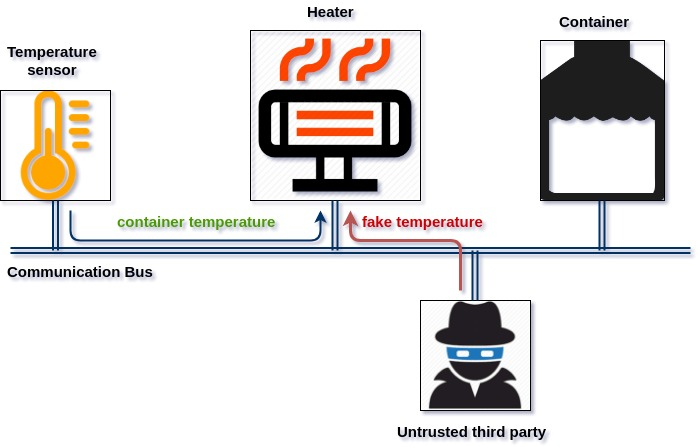
\includegraphics[width=12cm,height=6.5cm]{figures/general_intro/problematic.jpg}
\caption{Lack of authentication exploit}\label{vulnerablenetwork}
\end{figure}

\section{Objective and Proposed Solution}

SafetyNETp is an Industrial Ethernet protocol which provides two communication models, \ac{RTFN} and \ac{RTFL}.
\ac{RTFN} and \ac{RTFL} use different network topologies and operate on different
levels in the \ac{OSI} model. \ac{RTFN} operates on top of both layer two and four, whereas, \ac{RTFL} operates only on top of layer
two. The next chapter will exhibit the difference between these two variants and their respective communication models.
The \autoref{safetynetp_in_osi_model} shows the positioning of \ac{RTFN} and \ac{RTFL} in the \ac{OSI} model.

\begin{figure}[H]
\centering
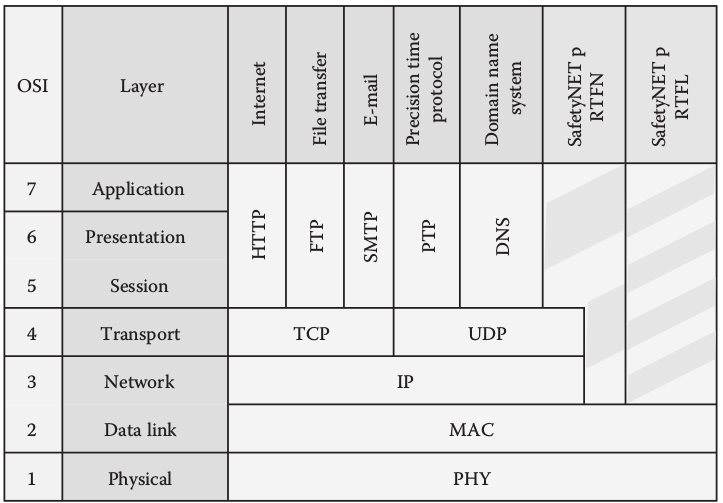
\includegraphics[width=12cm,height=7.5cm]{figures/safetynetp/safetynetp_in_osi_model.png}
\caption[SafetyNETp in the OSI reference model]{SafetyNETp in the \ac{OSI} reference model \cite{pilzSafetyNETpForRealTimeEthernet}}\label{safetynetp_in_osi_model}
\end{figure}
This project aims at securing SafetyNETp RTFN based communication, RTFL being out of the scope of this work; It consists of providing the three basic
security services which are confidentiality, integrity, and authenticity.
Designing a security layer from scratch is a hard and a very error-prone task. That's why we will be interested in the
available solutions which are already tested and assessed by the internet community. \ac{TLS}, \ac{DTLS} and \ac{IPsec} are the most
widely deployed protocols for securing network traffic.
As cited in the general introduction, \ac{TLS} is mostly used for securing
web traffic and e-mail protocols. \ac{TLS} can provide confidentiality, integrity, and authenticity by inserting it between the transport
and the application layers. However, \ac{TLS} provides these security services only for reliable transport protocols such as \ac{TCP}.
The incompatibility of \ac{TLS} with unreliable protocols led to the introduction of \ac{DTLS} which was introduced to provide \ac{TLS}'s security services for unreliable protocols.
Like \ac{TLS} and \ac{DTLS}, \ac{IPsec} provides confidentiality, integrity and authenticity, furthermore, it could be used for securing both
reliable and unreliable protocols.
In the next chapter, we study and we choose the suitable protocol to be used. Our solution consists of
designing and implementing a security layer for SafetyNETp RTFN based on the chosen security protocol.

Our work will involve the following steps :
\renewcommand{\labelitemi}{$\bullet$}
\begin{itemize}
\item Study SafetyNETp protocol
\item Study the available security solutions (\ac{TLS}, \ac{DTLS}, \ac{IPsec}) and choose the suitable one for SafetyNETp
\item Find and analyze the existing implementations of the protocol of choice and select the suitable one
\item Design the security layer and its integration into SafetyNETp
\item Implement and integrate the security layer
\item Test the implemented solution
\end{itemize}

\section*{Conclusion}

After setting the general context, we move in the following chapter to
outline the basic concepts needed for our project and to choose the security
protocol to be used

%_____________________________________________________________________________________
%
%       Filename:  chapter2.tex
%
%    Description:  Thesis Template HS Offenburg
%
%
%         Author:  Okba ZOUEGHI, okba.zoueghi@gmail.com
%     Supervisor:  Andreas Walz, Chadlia Jerad
%   Organization:  HS Offenburg, Offenburg, Germany
%
%_____________________________________________________________________________________

\chapter{State of the art}
\label{chap:chapter2}

Using one of the available security protocols, our project aims to secure SafetyNETp \ac{RTFN} based communication.
Therefore an overview and a description of those concepts are required. As SafetyNETp is an Industrial network protocol, we start the chapter with an overview of the history of industrial networks, then
we introduce SafetyNETp protocol and its communication models. Finally, we go through an overview of
the security protocols to choose the suitable one for our project.


\section{Industrial Networks} % (fold)
Nowadays we could not imagine a world without emails, online newspapers, blogs,
chat and the other services offered by the internet.
All these services are made possible thanks to the development of networking.
Networking plays an important role not only in our daily lives but also in
manufacturing and process automation. Unlike the networks that we are used to
in our daily lives, where devices like mobile phones, TVs, printers, and
computers are interconnected, in the industry, other types of devices are
interconnected such as sensors, motors, actuators, robots and similar other
devices. Hence we can speak about industrial networks.

The industrial systems faced the needs for improvement in production
monitoring and quality control and at the same time maintaining
the costs of all this as low as possible. This happened in the
last few decades due to the growth of social needs, which in turn enforce
the industrial systems to grow to match up with these needs.
So any operation that runs manually had to be replaced with a faster, and more
reliable automated operation. This provides the factories with
the necessary monitoring which allows better supervisory and quality control.
Introducing all this number of automated units into the factories needed an efficient
method to connect them together, to communicates with each other, and to transfer the
various supervisory data to the monitors.

Ethernet and Fieldbus are the two big keywords when it comes to industrial communication systems.
In this section, we go into an overview in which we see the evolution
of the industrial networks across the time \cite{zurawski2014industrial}.



% \subsection{Fieldbus systems}
%
% The word Fieldbus is basically the combination of two terms, field and bus.
% The meaning behind field as defined in the industrial word is a geographical area or space in which the industrial instruments such as sensors and actuators are situated and working. These industrial instruments' tasks are performed in the field level, hence they are commonly called field devices.
%  Regarding the term bus, in computer science, it refers to a line
% which allows connecting several units and permits to transfer
% data through it. Before going more into Fieldbus systems, let's
% see first how was the industrial networks before their introduction \cite{zurawski2014industrial}.
%
%
%
% In the industrial world like it shows the \autoref{Centralized_point-to-point_architecture}, the first solution that has been used for connecting field devices
% was parallel wiring or in other words star topology \cite{zurawski2014industrial}. Every field device is wired
% to a control computer which performs the control and the monitoring tasks. In order to perform these tasks, the
% control computer needs to transfer the data back and forth from the field devices using the traditional
% point-to-point technology. This architecture presents several
% disadvantages, it demands a high cost because of the point-to-point wiring, every field device needs to be wired
% separately to the control computer, moreover, If this control computer goes down all the system will collapse.
%
% \begin{figure}
% \centering
% 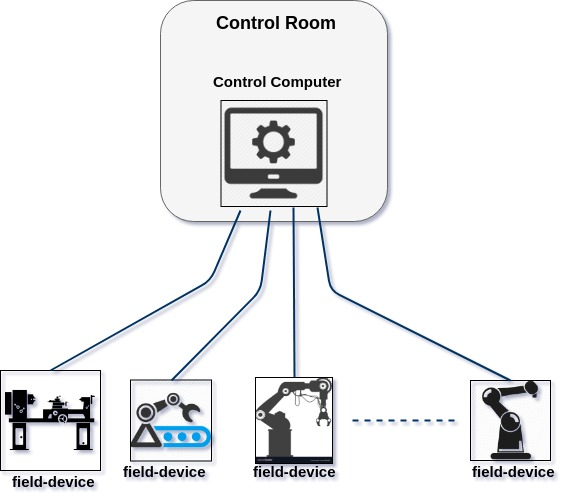
\includegraphics[width=12cm,height=8cm]{figures/fieldbus/star_topology_used_up_to_1960.jpg}
% \caption{Centralized point-to-point architecture}\label{Centralized_point-to-point_architecture}
% \end{figure}
%
% As a second step, unlike the previous solution which relies on a centralized control, In order to reduce the system fault,
% the new architecture includes more than one control computer \cite{zurawski2014industrial}. Each control computer controls and supervises a group
% of field devices, hence the risk of system fault is decreased. The \autoref{Decentralized_point-to-point_architecture}
% shows an example of a decentralized architecture.
%
% \begin{figure}
% \centering
% 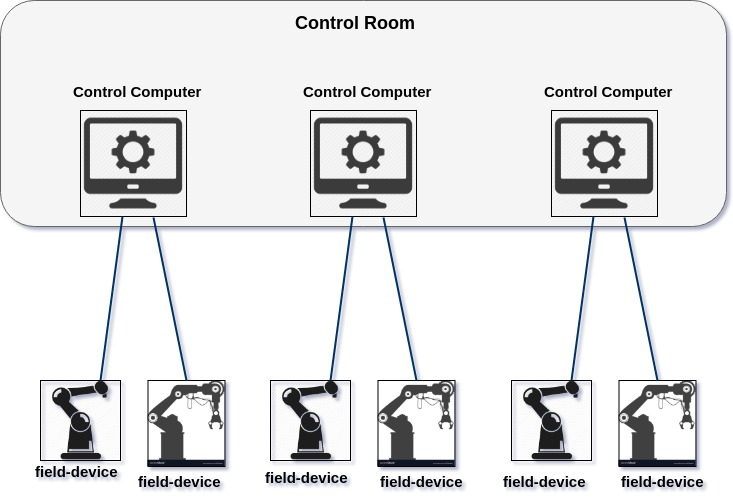
\includegraphics[width=12cm,height=8cm]{figures/fieldbus/decentralized_topology.jpg}
% \caption{Decentralized point-to-point architecture}\label{Decentralized_point-to-point_architecture}
% \end{figure}
%
% Each step aims to reduce the costs compared with the previous one. After the decentralization of control devices, In order to reduce
% the wiring cost, a local control-device is installed next to each group of field devices \cite{zurawski2014industrial}. As
% shown in \autoref{Local_control_devices} each one of the control-devices controls and monitors a group of filed-devices. These
% control-devices are then wired to a central supervisory computer. This solution keeps the advantages of the
% previous ones, in addition, it significantly reduce the length of the wires which eventually reduce the cost with an important manner.
%
% \begin{figure}
% \centering
% 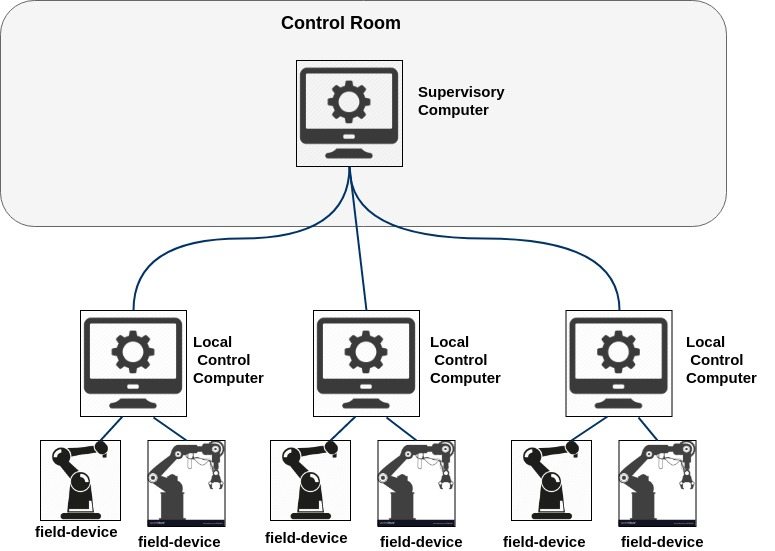
\includegraphics[width=12cm,height=7cm]{figures/fieldbus/local_control_devices.jpg}
% \caption{Local control devices}\label{Local_control_devices}
% \end{figure}
%
% After all this evolution, the point-to-point wiring problem is still present. The solution was the famous Fieldbus systems.
% The desire to cope with the wiring problem getting out of hand in large installations was certainly the main impetus for its development.
% Fieldbus systems were introduced in 1980 and the idea behind them is to connect all the field devices with one single link called Fieldbus \cite{zurawski2014industrial}.
% To be able to let all the field devices communicate and transfer data through one single line, a communication protocol should be used
% to manage the bus access. The communication protocol will be responsible to define a mechanism for acquiring the bus and devices synchronization.
% Hence the data transferred through the bus will be multiplexed in time. An example of a protocol that can be used for managing the Fieldbus access, the
% \ac{CSMA} protocol. The advantages introduced by the Fieldbus systems are many, the most important is the substantial reduction of wiring
% and adding more flexibility. With Fieldbus systems, the network extension is very much easier to achieve.
% For instance, CAN is one of the most well-known Fieldbus systems. It is mostly used in automotive networks.
% The \autoref{fieldbus_network} shows the architecture of a Fieldbus network.
%
% \begin{figure}
% \centering
% 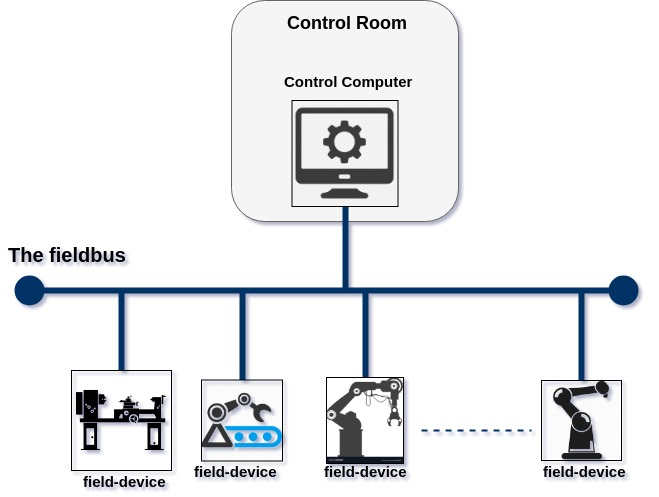
\includegraphics[width=12cm,height=7cm]{figures/fieldbus/fieldbus_network.jpg}
% \caption{Fieldbus network}\label{fieldbus_network}
% \end{figure}

\subsection{Fieldbus Systems}

The word Fieldbus is basically the combination of two terms, field and bus.
The meaning behind field as defined in the industrial world is a geographical
area or space in which the industrial instruments such as sensors and actuators
are situated and working. These industrial instruments' tasks are performed at the
field level, hence they are commonly called field devices.
Regarding the term bus, in computer science, it refers to a line
which allows connecting several units and permits to transfer
data through it. Before going more into Fieldbus systems, let's
see first how was the industrial networks before their introduction \cite{zurawski2014industrial}.

In the industrial world, as shown in \autoref{Centralized_point-to-point_architecture}, the first solution
that has been used for connecting field devices
was star topology \cite{zurawski2014industrial}. Every field device is wired
to a control computer which performs the control and the monitoring tasks. In order to perform these tasks, the
control computer needs to transfer the data back and forth from the field devices using the traditional
point-to-point technology. This architecture presents several
disadvantages, it demands a high cost because of the point-to-point wiring, every field device needs to be wired
separately to the control computer, moreover, if this control computer goes down, all the system will collapse.

\begin{figure}[!htbp]
\centering
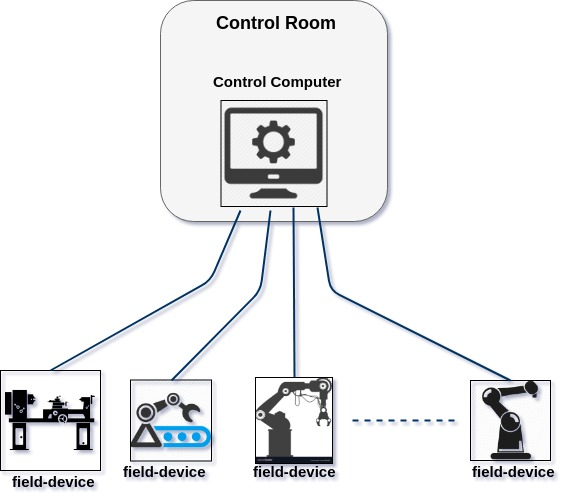
\includegraphics[width=9cm]{figures/fieldbus/star_topology_used_up_to_1960.jpg}
\caption{Centralized point-to-point architecture}\label{Centralized_point-to-point_architecture}
\end{figure}

The desire to cope with the wiring problem getting out of hand in large installations was certainly the main impetus
for the development of Fieldbus systems. Fieldbus systems were introduced in 1980 and the idea behind them is to connect all the field
devices with one single link called Fieldbus \cite{zurawski2014industrial}. To be able to let all the field devices
communicate and transfer data through one single line, a communication protocol should be used to manage the bus
access. The communication protocol is responsible for defining a mechanism for acquiring the bus.
Hence the data transferred through the bus will be multiplexed in time. An example of a protocol that can be used for
managing the Fieldbus access is the \ac{CSMA} protocol. The advantages introduced by the Fieldbus systems are many, the most
important is the substantial reduction of wiring and adding more flexibility. With Fieldbus systems, the network extension
is very much easier to achieve.
For instance, CAN is one of the most well-known Fieldbus systems. It is mostly used in automotive networks.
The \autoref{fieldbus_network} shows the architecture of a Fieldbus network.

In today's industrial networks, even systems using topologies other than the linear topology are still called Fieldbus systems.

\begin{figure}[!htbp]
\centering
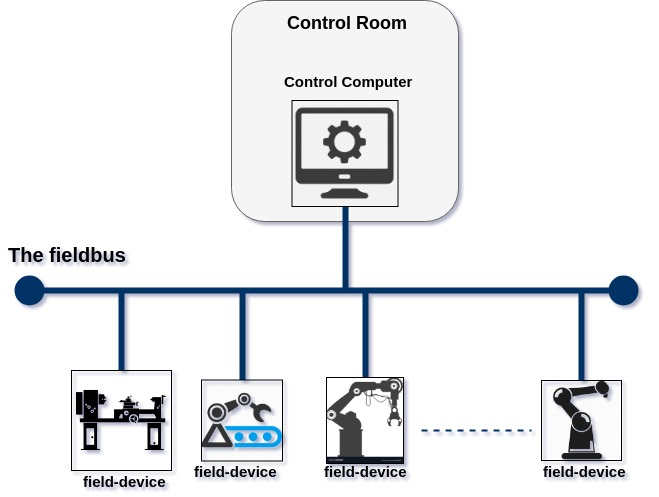
\includegraphics[width=9cm]{figures/fieldbus/fieldbus_network.jpg}
\caption{Fieldbus network}\label{fieldbus_network}
\end{figure}

\subsection{Industrial Ethernet}

Ethernet is a very important communication platform (a physical layer and a data link layer)
which was standardized by the \ac{IEEE} as IEEE 802.3 \cite{kunbusIndustrialEthernet}.
Ethernet is now the most popular and the most widely used network technology in the world which without
it, communication between devices in today’s modern world would not be possible. For instance, Ethernet
is used to connect devices in companies networks like printers and computers, to connect devices in
our houses, to connect servers, routers and plenty of other examples.

A key strength of Ethernet is that it enables to run many protocols simultaneously on the
same network also it provides flexibility and scalability in a way not seen before. With the
growth of Ethernet and having these advantages, the idea of using Ethernet in the industry was introduced.
This, in fact, enables a common communication platform for all industrial network protocols. Also, this makes possible to let the
field devices communicate with the office devices (using the \ac{TCP}/\ac{IP} model) which provides more
flexibility and scalability. Therefore, field devices control and monitoring are not only possible from
inside the plant, but also from outside. For instance, a web server could be installed on a field device
and could be accessed from an office device to monitor what is happening on the field level \cite{profinet2013ethernet}.

Unfortunately, when Ethernet was introduced, the transmission data rate was 10 Mbit/s which is not suitable for
industrial communication. This led to the development of what is called fast-Ethernet with transmission data
rates of 100 Mbit/s and 1 Gbit/s which is considered sufficient for industrial usage. Another issue is that
using Ethernet in the industry requires additional considerations not seen in Ethernet systems used in an
office. In fact devices in industrial environments are exposed to different temperatures, vibrations
and other potentially disturbing noises and movements \cite{kunbusIndustrialEthernet}.
% The wiring technology being used within Ethernet is RJ45
% which was developed for non-industrial communication. For this purpose, a new RJ45 with additional protection
% was developed in order to meet the requirements needed in industrial environments \cite{kunbusIndustrialEthernet}.

As we know, in industrial applications, the real-time performance highly matters and has a considerable effect on
the automated process. As we discussed previously, using Ethernet in the industry enables the communication
between the office devices and the field devices. This is, of course, possible using the \ac{TCP}/\ac{IP} communication model. Unfortunately, \ac{TCP}/\ac{IP}
could not be fast enough to satisfy some applications with tight and critical time requirements. In fact, when data is sent using  \ac{TCP}/\ac{IP}, like \autoref{data_encapsulation_for_non_critical_time_applications} shows, the data is packed
into the application layer then into the transport layer which basically \ac{TCP}   or \ac{UDP} then packed into \ac{IP} datagram and
finally into Ethernet frame. When the Ethernet frame is received, the previously cited layers need to be unpacked in
order to get the data. The operation of packing and unpacking data through several layers consumes a considerable amount
of time that's why alongside using \ac{TCP}/\ac{IP} another approach is commonly used in order meet the requirements of
critical-time applications. The idea behind this approach is basically to minimize the number of packing and unpacking
operations by skipping the network and transport layers (\ac{IP}  and \ac{TCP}   /\ac{UDP}) which significantly increases the
performance. The \autoref{data_encapsulation_for_critical_time_applications} illustrates the second approach \cite{profinet2013ethernet}.
\begin{figure}
\centering
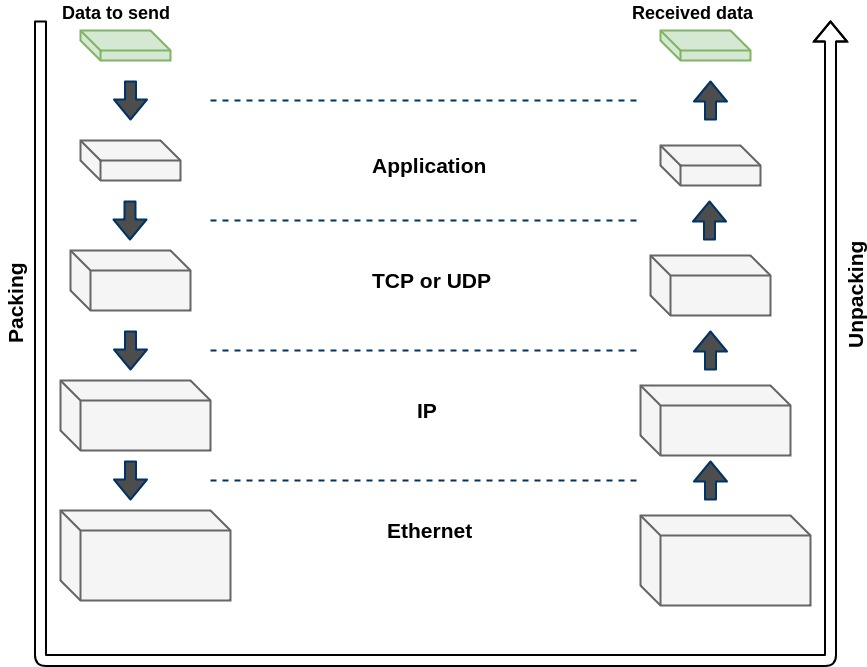
\includegraphics[width=12cm,height=8cm]{figures/indutrial_ethernet/data_encapsulation_for_non_critical_time_applications.jpg}
\caption{Data encapsulation for non-critical-time applications}\label{data_encapsulation_for_non_critical_time_applications}
\end{figure}

\begin{figure}
\centering
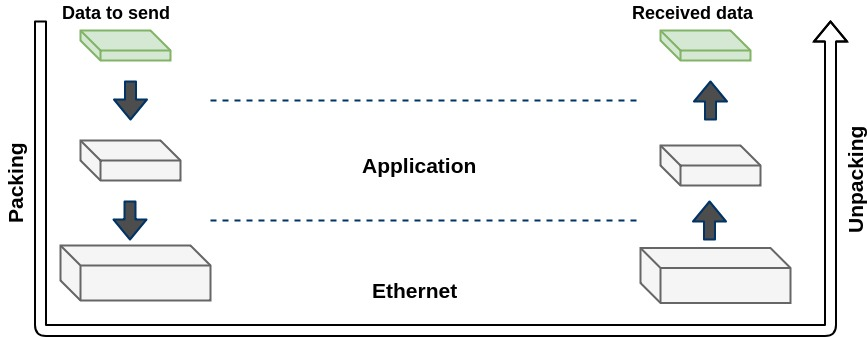
\includegraphics[width=12cm,height=6cm]{figures/indutrial_ethernet/data_encapsulation_for_critical_time_applications.jpg}
\caption{Data encapsulation for critical-time applications}\label{data_encapsulation_for_critical_time_applications}
\end{figure}

\section{SafetyNETp protocol}
\label{SafetyNETp}
SafetyNETp is a communication protocol developed by Pilz GmbH & Co. KG, which allows the
construction of industrial Ethernet-based networks and is suitable for both real-time communications and
safety-oriented applications. The meaning of safety does not refer to networking security, however, it
refers to safety applied to humans and to the environment. SafetyNETp is used wherever the temporal and content
consistency of communicated data is required to hedge dangers. The dangers can be the endangering of lives as well as the plant assets.
The second field of application is the communication of data in real time. With bus cycle times of
up to 62.5 microseconds, SafetyNETp can be used even in extremely time-critical areas.
Typical fields of application are factory automation (e.g. automobile production), transport
technology (e.g. cable cars). In general, all applications of automation and process technology are
possible \cite{KunbusSafetyNETp}.


The protocol enables the transmission of safety-related data on the same
cable used for the transfer of control or process data. In fact, it can
be used to transfer safety data without the need for a physical dedicated communication line.
Combining safe and nonsafe communications over the same medium have several advantages. First of
all, the reduced amount of cables needed to connect the network elements makes the wiring of components simpler, thus reducing costs for setup and maintenance. Moreover, the ability to connect safe
and nonsafe devices to the same network makes a number of non-safety-related functions (e.g. remote
diagnostic, data logging) available for safe devices and at the same time allows standard devices to
access safety data \cite{zurawski2014industrial}.

The communication mode commonly used in the industry is the Master/Slave mode. Within
this mode, the master can request to read a value from a slave or also write a value to it.
The slaves can't communicate directly with each other, they just respond to the read
requests sent by a given master and apply the received commands. Hence this mode
requires always a centralized controller. The \autoref{master-slave-mode} shows an example
of Master/Slave communication \cite{JonasFieldbus}.

\begin{figure}[H]
\centering
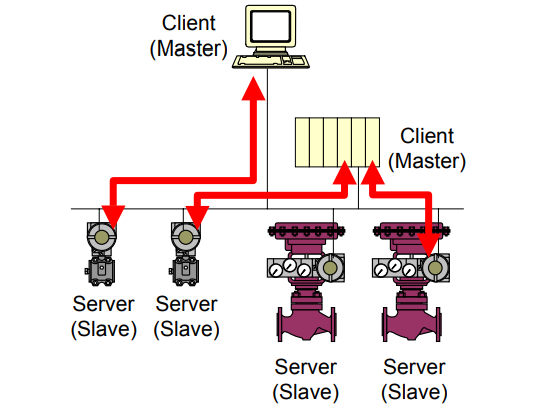
\includegraphics[width=10cm,height=4.6cm]{figures/safetynetp/master-slave-mode.png}
\caption[Master/Slave communication]{Master/Slave communication \cite{JonasFieldbus}}\label{master-slave-mode}
\end{figure}

In order to avoid the need for a centralized device and to make the data available to
all devices, SafetyNETp uses a multi-master bus system where all devices are given the same rights \cite{zurawski2014industrial}. It uses
a Publisher/Subscriber mode, where each device publishes its relevant data and can subscribe, at the same time,
the reception of data needed to carry out its tasks, which are produced by other entities in the network.
The \autoref{publish-subscribe-mode} shows an example of Publish/Subscribe communication.

\begin{figure}[H]
\centering
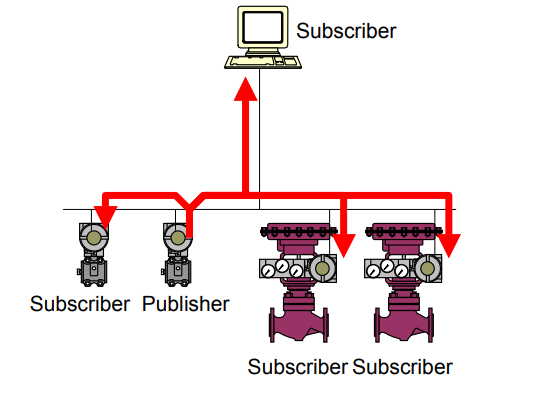
\includegraphics[width=10cm,height=6cm]{figures/safetynetp/publish-subscribe-mode.png}
\caption[Publish subscribe communication]{Publish subscribe communication \cite{JonasFieldbus}}\label{publish-subscribe-mode}
\end{figure}

As cited in the first chapter, SafetyNETp provides two communication models \ac{RTFN} and \ac{RTFL}. In the next sections, we present the
frame layout of both \ac{RTFN} and \ac{RTFL}, a brief overview about \ac{RTFN} and a detailed explanation of \ac{RTFN}.

\subsection{Frame layout}

As the \autoref{safetynetp_in_osi_model} shows, \ac{RTFN} runs on top of \ac{UDP} and \ac{RTFL} runs on top of Ethernet. Therefore \ac{RTFN}'s application
data represents \ac{UDP}'s payload and \ac{RTFL}'s application data represents Ethernet's payload. The SafetyNETp header is a one-byte
field which indicates the frame type or in other words the payload's content.

\begin{figure}[H]
\centering
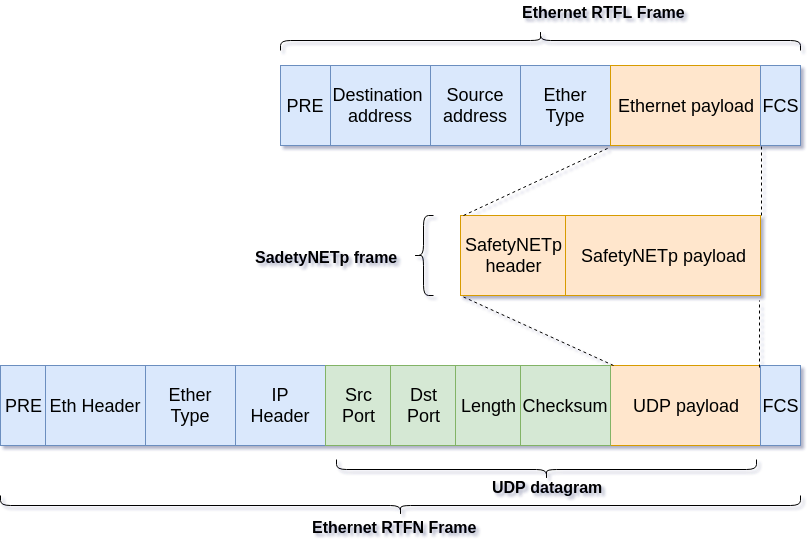
\includegraphics[width=10cm,height=8cm]{figures/safetynetp/safetynetp_frame_layout.png}
\caption{Mapping of SafetyNETp frame into Ethernet frame and UDP datagram}\label{frame-layout}
\end{figure}

\subsection{RTFL}

\ac{RTFL} has been designed for applications where real-time performance is of primary
importance. It is based on a linear topology, and the transport of data is supported through
standard Ethernet (OSI layer 2) frames. This communication model enables a minimum bus scan
time of 62.5 microsecond and limits jitters to 100 nanoseconds or less, making the protocol suitable for highly demanding
control applications \cite{zurawski2014industrial}. The reasoning behind skipping the network and the transport layers is to
increase the performance and this is achieved by reducing the time of packets processing (packing and unpacking).
\ac{RTFL} uses the linear topology which in fact keeps the advantages of Fieldbus systems. All devices are
connected through one single line which reduces the wiring costs and makes the data available for all devices.

As shown in \autoref{rtfl-physical-line}, in an \ac{RTFL} network, the communication is initiated by a special device called root device (RD). At each communication
cycle, the RD creates an \ac{RTFL} Ethernet frame and sends it along the line. All the cascading devices, also known as ordinary devices (ODs), append their data to the frame. When the frame reaches the end
of the line (last device), it is forwarded on the way back to the RD. While traveling in this direction, relevant
data are then read by the different ODs. Each \ac{RTFL} network requires just one RD.

\begin{figure}[H]
\centering
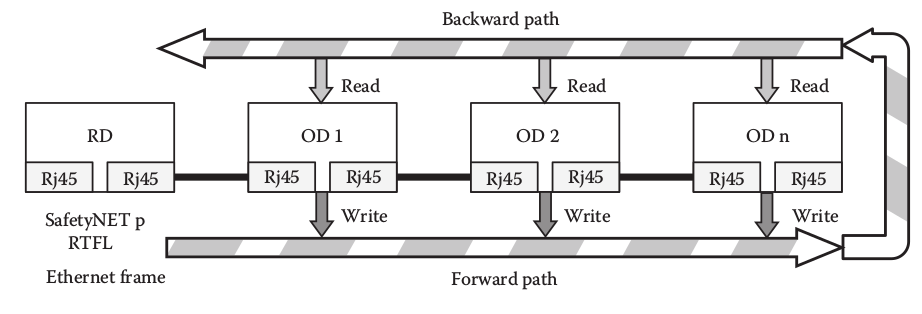
\includegraphics[width=10cm,height=5cm]{figures/safetynetp/rtfl-physical-line.png}
\caption{RTFL physical line}\label{rtfl-physical-line}
\end{figure}

\ac{RTFL} is designed to minimize the overhead by using frames as common containers for data from all devices.
As depicted in \autoref{rtfl-ethernet-frame} a single Ethernet frame can carry all process data needed by the devices. Minimizing the header overhead is important to reach
cycle times as short as 62.5 microseconds, which are needed especially in motion control applications.

\begin{figure}[H]
\centering
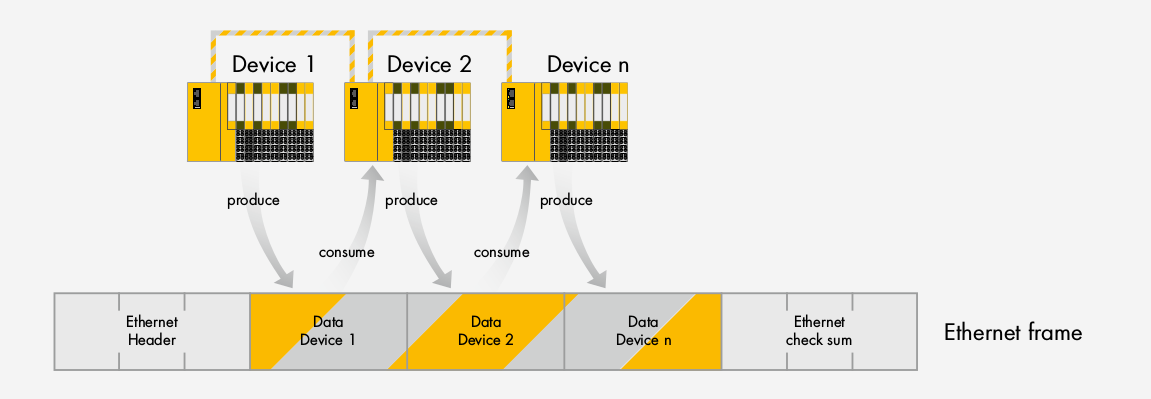
\includegraphics[width=15cm,height=5cm]{figures/safetynetp/rtfl-ethernet-frame.png}
\caption{RTFL Ethernet frame}\label{rtfl-ethernet-frame}
\end{figure}

\subsection{RTFN}

When real-time requirements are not so tight and a cycle time over 1 millisecond is sufficient, the \ac{RTFN} communication model
can be used to obtain the maximum degree of flexibility and integration with other
standard Ethernet-based protocols likely adopted at higher levels of the factory hierarchy. In fact, \ac{RTFN}
can use the standard \ac{UDP}/\ac{IP}  protocols to transport data, allowing both the routing of frames among
different networks and the integration with the existing communication infrastructures. \ac{RTFN}
can be used for communication between field devices and for connecting the field devices to
the office network. \ac{RTFN} is compatible with \ac{RTFL} and it can be used to connect multiple \ac{RTFL} networks together.
\ac{RTFN} does not restrict the usage of a specific topology, it allows using any network topology, for
instance, star, tree and ring topologies.

\ac{RTFN} follows a Publish/Subscribe communication model where the data is exchanged through
the concept of topics. An \ac{RTFN} device could be a publisher, a subscriber or both together.
Each publisher has a list of topics. When a publisher receives a \textit{subscribe request} for a topic it has,
it responds by sending data about the subscribed topic to the subscriber and this is called publishment.
For instance, a temperature sensor could be a publisher which has the temperature as a topic. A device
could get the temperature value by subscribing to the corresponding topic.
In an \ac{RTFN} network, as it is shown in \autoref{rtfn-frame-and-messages-type}, six types of messages
could be exchanged between devices:
\begin{itemize}
\setlength{\labelwidth}{10pt}
  \item Subscribe request: used by subscribers to request the subscription for a specific topic.
  \item Subscribe acknowledgment: used by a publisher to confirm that a subscription request has been accepted.
  \item Unsubscribe request: used by a subscriber to unsubscribe the reception of some topic.
  \item Still alive: sent by a subscriber to a publisher to inform it that it is still alive.
  \item Unpublished: sent by a publisher to a subscriber to inform it that no more data will be received for a certain topic.
  \item Cyclic data: message sent cyclically by the publisher to the subscriber which contains topics' data.
\end{itemize}

\begin{figure}[H]
\centering
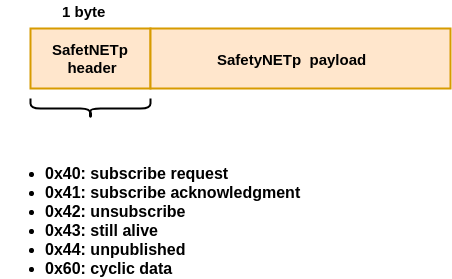
\includegraphics[width=10cm,height=4cm]{figures/safetynetp/rtfn-frame-and-messages-type.png}
\caption{RTFN frame and messages type}\label{rtfn-frame-and-messages-type}
\end{figure}

The sequence diagram shown in \autoref{rtfn-pub-sub} illustrates the subscription and the publishment process. In this
diagram, for simplicity reasons, we assume that the messages are sent reliably (no message loss). The publisher and the
subscriber don't know each other in advance, that's why the subscriber starts by sending a \textit{subscribe request} as broadcast (the \textit{subscribe request}
will be sent to all the devices in the network). The devices present in the network will receive the \textit{subscribe request} and
the device which has the topic available will send back a \textit{subscribe acknowledgment} as unicast to the subscriber.
Once the subscription process has finished, the publisher starts publishing cyclically data about the corresponding topic to the subscriber.
The published data is called \textit{cyclic data} and sent only to the subscriber. The subscriber also
sends cyclic messages to the publisher. These messages consist of \textit{still alive} messages that are sent in order to inform the publisher that the subscriber is still alive.

\begin{figure}[H]
\centering
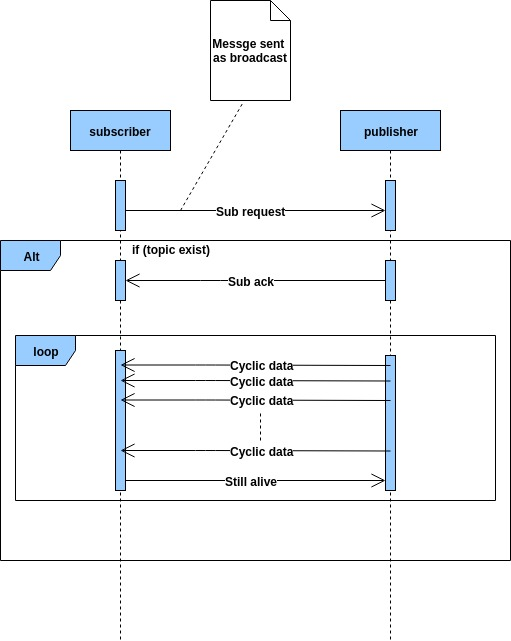
\includegraphics[width=10cm,height=9cm]{figures/safetynetp/rtfn-pub-sub.jpg}
\caption{RTFN Publish/Subscribe communication}\label{rtfn-pub-sub}
\end{figure}

The publisher can stop sending \textit{cyclic data} to the subscriber for multiple reasons.
If the subscriber is down, the publisher will not receive anymore \textit{still alive} messages, therefore
it will stop sending \textit{cyclic data}.
The subscriber can send an \textit{unsubscribe request} to the publisher in order to inform it that the cyclic
data for some topic is not needed anymore. The publisher will stop sending \textit{cyclic data} upon receiving the \textit{unsubscribe request}, moreover,
the publisher also can send an \textit{unpublished} message to the subscriber to inform it that no more \textit{cyclic data} will be published
for a certain topic.

For simplicity reasons, we assumed that there is no message loss. However as we mentioned before,
\ac{RTFN} uses \ac{UDP} as a transport layer which does not provide reliable transfer. What will happen if for
example the \textit{subscribe acknowledgment} sent by the publisher is lost? In fact, the subscriber will keep
sending always \textit{subscribe requests} until receiving a \textit{subscribe acknowledgment} from the publisher.

\section{Security Protocols}

In today's internet, almost everything is based on the \ac{TCP}/\ac{IP} model. The internet was primarily a small network
connecting a community of researchers, but with the success of \ac{TCP}/\ac{IP} the internet expanded to become a gigantic global
network connecting devices of all types. With the huge success of \ac{TCP}/\ac{IP} and the growth of the internet, \ac{TCP}/\ac{IP} application
became attractive for the industry and the automation area (e.g. Industrial Ethernet).
However, no security measures were taken into consideration while designing \ac{TCP}/\ac{IP} as it was only for
interconnecting small and private networks. In this section, we discuss the most common \ac{IP} security
measures.

\subsection{Secure Sockets Layer/Transport Layer Security}

% Today with the growth of the internet, we can do a lot of things from our mobile phones or PCs.
% We are able to send e-mails, files, photos and share all kind of data between our devices. We can
% buy products or even it's possible to perform money transactions through the internet. With the introduction of IoT,
% one can speak about smart houses. Everything in our houses can be commanded remotely. It
% is good to have all these services, unfortunately, without security measures, it can lead to
% crucial problems. That's why SSL/\ac{TLS} (Secure Sockets Layer/Transport Layer Security) protocol was introduced to solve the security problems.

\ac{SSL}/\ac{TLS} is the most widely deployed protocol for
securing network traffic. It is widely used for protecting Web traffic and for e-mail protocols such as
Internet Message Access Protocol (IMAP) and Post Office Protocol (POP). \ac{TLS} is developed for any reliable transport
protocol which maintains the messages' order. It is typically used for securing \ac{TCP} applications (e.g. HTTP).

\subsubsection{Introduction and History}

The first \ac{SSL} version was introduced by Netscape in 1994. In 1995 and 1996, \ac{SSL} versions 2.0 and 3.0 were released
and then came the release of \ac{TLS} 1.0 which is, in fact, the same as \ac{SSL} 3.1. Basically, there is no
difference between \ac{TLS} and SSL, beginning from \ac{SSL} version 3.1, the protocol name has been changed
to become \ac{TLS} 1.0 \cite{SSLHistory}. The last standardized \ac{TLS} version today is 1.2 which was released in 2008 in RFC5246 \cite{rfc5246}
, moreover, drafts are available for \ac{TLS} version 1.3. The last published draft of \ac{TLS} 1.3 was on 20 March 2018 \cite{draftTLSv1.3}.

The goal of SSL/\ac{TLS} is to provide the three crucial security services:

\begin{itemize}
\setlength{\labelwidth}{10pt}
  \item Confidentiality: the data is sent encrypted and only the devices which have the keying material could decrypt and read the data.
  The encryption is performed via symmetric encryption algorithms such as \ac{DES} or \ac{AES}.

  \item Integrity: communication partners can detect changes to a message during transmission.
  this is achieved using \ac{MAC}.

  \item Authentication: the recipient of a message can identify its communication
partner and can detect if the received message has been forged. The authentication
is likely based on a pre-shared key or on client's and server's certificates.
\end{itemize}

\ac{TLS} is based on a sub-protocol named record layer protocol which on
top of it we can find four protocols, the Handshake protocol, the Change Cipher Spec protocol,
the Alert protocol and the Application Data protocol (\autoref{tls-protocol-architecture}). Among these four protocols, the most
important one is the Handshake protocol which is used for establishing an authenticated
cryptographic secret between two endpoints by commonly using public key cryptography \cite{rfc5246}.

\begin{figure}[H]
\centering
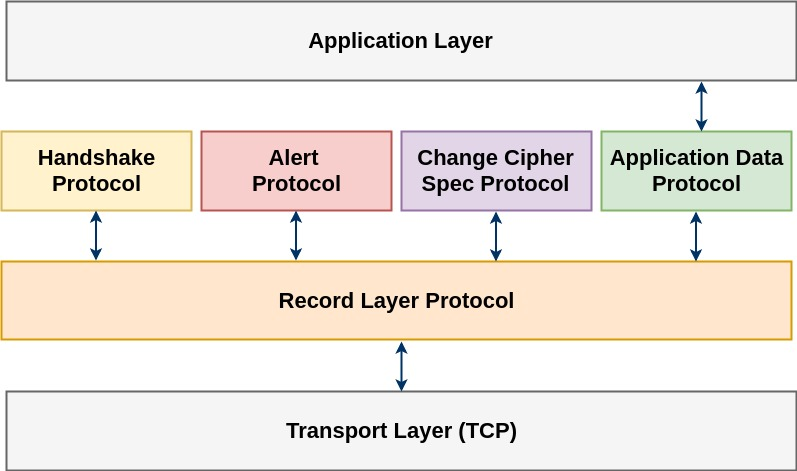
\includegraphics[width=10cm,height=6cm]{figures/dtls/tls-protocol-architecture.jpg}
\caption{TLS protocol architecture}\label{tls-protocol-architecture}
\end{figure}

\subsubsection{\ac{TLS} Handshake}

\ac{TLS} is designed to work on top of a reliable transport protocol typically \ac{TCP}. It follows the Client/Server
communication model and its goal is to establish a secure connection between a server and a client
and let them exchange data securely across an untrusted network. To establish a secure connection, the \ac{TLS} handshake needs to take
place. During the handshake, important messages are exchanged between the client and the server. With the messages exchanged
the client and the server basically agree on the protocol version, select the encryption and the MAC algorithms,
authenticate each other by exchanging and validating digital certificates and share a symmetric encryption key to be used
for encryption \cite{rfc5246}.

\begin{figure}[!htbp]
\centering
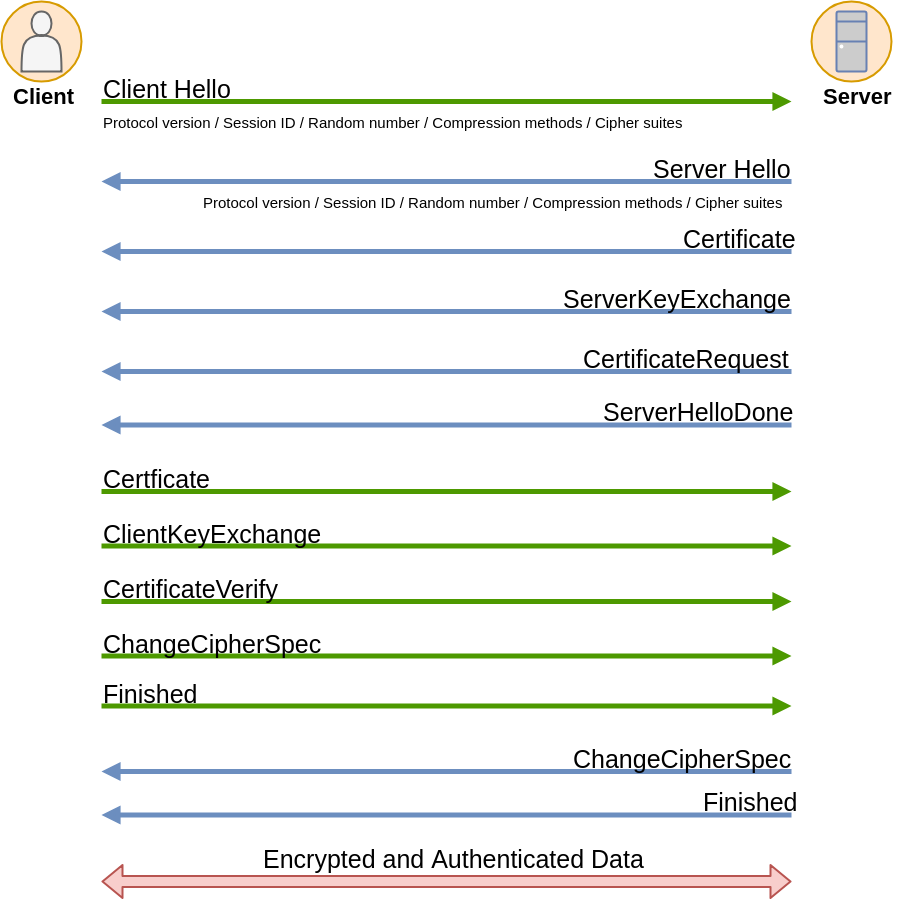
\includegraphics[width=11cm,height=14cm]{figures/dtls/tls-handshake.png}
\caption{SSL/TLS full handshake}\label{tls-handshake}
\end{figure}


As standardized in RFC5246 \cite{rfc5246}, a full SSL/\ac{TLS} handshake contains the following messages (\autoref{tls-handshake}):

\begin{itemize}
\setlength{\labelwidth}{10pt}
  \item Client Hello: it is the first handshake message and it is sent from the client to the server.
  It contains the supported \ac{SSL} and \ac{TLS} versions, a random number, a session id and the supported compression methods and cipher suites. In fact, cipher suites are very important
  as they define the key exchange algorithm, the authentication algorithm (digital signature algorithm),
  the data encryption algorithm as well as the MAC algorithm (\autoref{tls-cipher-suite-example}).

  \begin{figure}[H]
  \centering
  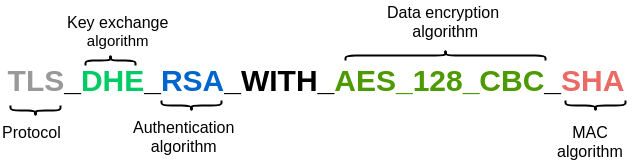
\includegraphics[width=10cm,height=2.5cm]{figures/dtls/tls-cipher-suite-example.png}
  \caption{TLS cipher suite example}\label{tls-cipher-suite-example}
  \end{figure}

  \item Server Hello: upon receiving the Client Hello, the server sends back the Server Hello message
  which contains the selected parameters (key exchange algorithm, the authentication algorithm...).

  \item Server Certificate: it is optional to send, it lets the client verify the identity of the server.

  \item Server Key Exchange: this message is not always present in the handshake, it is only sent if
  the server certificate is not sufficient to allow the client to exchange the secret key.

  \item Certificate Request: it is optional to send, it informs the client to provide its certificate
  for authentication.

  \item Server Hello Done: sent by the server to indicate the end of the Server Hello and the associated messages
  (Server Certificate, Server Key Exchange, and Certificate Request). Upon receiving the Server Hello done, the client verifies the validity of the server certificate and the parameters selected by the server in the Server Hello.

  \item Client Key Exchange: it is sent by the client after receiving the Server Hello Done to set the \ac{PMS}. The content of this messages depends on the selected key exchange algorithm, if RSA is chosen,
  the PMS is encrypted against the server's public key, however, if \ac{DH} is chosen, DH parameters will be sent. The PMS secret will be used on both sides to compute a shared \ac{MS} which will be used for encryption, decryption and MAC calculation.

  \item Client Certificate: sent if required by the server, it allows the server to verify the identity of the client.

  \item Certificate Verify: if the client sends a certificate with signing ability, a digitally-signed Certificate Verify message is sent in order to explicitly verify the certificate.

  \item Change Cipher Spec: sent by both the client and the server. This message indicates that the following messages
  will be sent encrypted using the shared keying material.

  \item Finished: sent by both the client and the server after the Change Cipher Spec message to verify that the key exchange and authentication processes were successful. It is the last handshake message and the first encrypted one.

\end{itemize}


\subsubsection{How the security services are ensured?}

In our project, when we say security services, we mean basically confidentiality, integrity, and authenticity.
When the server sends its certificate, the client verifies the validity of the certificate using the public key of the
\ac{CA}. If the certificate is valid, the client generates a PMS and sends it to the server.
Not only the client can verify the server identity, also the server verifies the client identity, in the same way, using
the client certificate. If the client certificate is valid the server will accept the provided PMS.
Using the PMS, both the client and server derive a MS which is in turn used to derive other several keys.
These keys are used for exchanging authenticated and encrypted data with the capability to the check its integrity.
The confidentiality is ensured by encrypting the data, the authentication and the integrity are both ensured using a MAC algorithm \cite{rfc5246}.


\subsection{Datagram Transport Layer Security}

A lot of applications today in several domains are delay sensitive and have tight time constraints.
For instance, we can speak of industrial communication, IoT, internet telephony, online gaming and several other applications.
Due to the time constraints, for this kind of applications \ac{UDP} is used instead of \ac{TCP}   .

\subsubsection{Introduction and History}

Application layer protocols that work on top of \ac{TCP} such as Hypertext Transfer
Protocol (HTTP), Secure Shell (SSH) or File Transfer Protocol (FTP) can be easily secured using
\ac{TLS} as it is designed to secure applications working on top of a reliable transport protocol. Unfortunately,
for datagram based applications, no such alternative exists. Therefore, similarly to TLS, DTLS
was introduced to allow the use of the same security services provided by \ac{TLS} but for datagram based applications.

Over the years, \ac{TLS} has become more robust and has been refined to withstand numerous attacks that's why
\ac{DTLS} was designed to be as similar as possible to it. By minimizing the changes, the risk of introducing new weaknesses
or vulnerabilities will be reduced. Moreover, \ac{DTLS} implementation will be easier by reusing \ac{TLS} pre-existing infrastructure \cite{designAndImlementationOfDTLS}.

The last standardized \ac{DTLS} version is 1.2, it was standardized in 2012 as RFC6347 \cite{rfc6347}. Like TLS,
drafts have been published for \ac{DTLS} version 1.3. The last draft was published on 02 July 2018 \cite{draftDTLSv1.3}.

\subsubsection{\ac{DTLS} Design}

\ac{TCP}   provides a reliable bi-directional tunnel for bytes, where all bytes eventually reach the receiver
in the same order as what the sender used to send them. \ac{TCP} achieves that through a complex
assembly of acknowledgment messages, transmission timeouts and retransmission. As \ac{TLS} uses \ac{TCP},
it does not encounter issues related to packet loss and reordering which is not the case for DTLS.

The unreliability of datagram protocols creates problems for \ac{TLS} in two levels.
First, the messages decryption is dependent from the previous messages as the integrity check is based on the
implicit sequence number. If record N is not received, then the integrity check
on record N+1 will be based on the wrong sequence number and
thus will fail. Second, \ac{TLS} assumes that the handshake messages are sent reliably, hence,
the connection cannot be established if a handshake message is lost \cite{rfc5246}.

In order to handle packet loss, \ac{DTLS} uses a retransmission timer described in details in RFC6347 \cite{rfc6347}.
\ac{DTLS} includes an explicit sequence number which is used
for MAC calculation. It is used also to detect replay attacks and reordering. Furthermore, a new field was introduced named epoch which is incremented each time a CipherChangeSpec
message is sent.

Some \ac{TLS} cipher suites retain a cryptographic context between records which
does not allow to process individual records. This will cause problems with
unreliable protocols, therefore, \ac{DTLS} banned the usage of this kind of cipher suites \cite{rfc5246}.

\ac{TLS} and \ac{DTLS} handshakes are the same except that \ac{DTLS} has introduced a new message which does not
exist in \ac{TLS}'s handshake. The new message is named Hello Verify Request, it contains a cookie and it is sent back
to the client just after receiving the Client Hello message. the client should send back another Client Hello
which contains the same cookie. If the cookie is verified the handshake will continue (same \ac{TLS} handshake steps), otherwise,
the server will close the connection. The cookie mechanism allows reducing the risk of \ac{DoS} attacks.
No such message exists in \ac{TLS} handshake because the \ac{TCP}   handshake is established before starting the \ac{TLS} handshake
which will make the DoS attack difficult. This is not the case for datagram protocols because no connection is established prior to
the \ac{DTLS} handshake, hence, the cookie mechanism is needed \cite{rfc6347}.

\subsection{Internet Protocol Security}

\ac{IPsec} is a protocol suite which was introduced to secure network traffic and more specifically \ac{IP} and its
upper layers protocols, typically \ac{TCP} or \ac{UDP}. \ac{IPsec} is situated in layer three of the OSI model and it offers data
integrity, replay protection, authentication, and confidentiality natively within the \ac{IP} layer. \ac{IPsec}
offers two communication modes, tunnel mode and transport mode (\autoref{ipsec_communication_modes}).
The tunnel mode provides network-to-network security whereas the transport mode provides host-to-host security.
In fact, in the tunnel mode, the sender sends the message as it is (unprotected) to the gateway, then the gateway encapsulates the message
and sends it securely. The receiving gateway decapsulates the secured message and passes the original message to the receiver if
the message is verified correctly (e.g. integrity, authentication). In the transport mode, unlike the tunnel mode, protecting
the messages is no longer performed by the gateway, instead, the end hosts manage themselves to secure and verify the messages.

 \begin{figure}[!htbp]
 \centering
 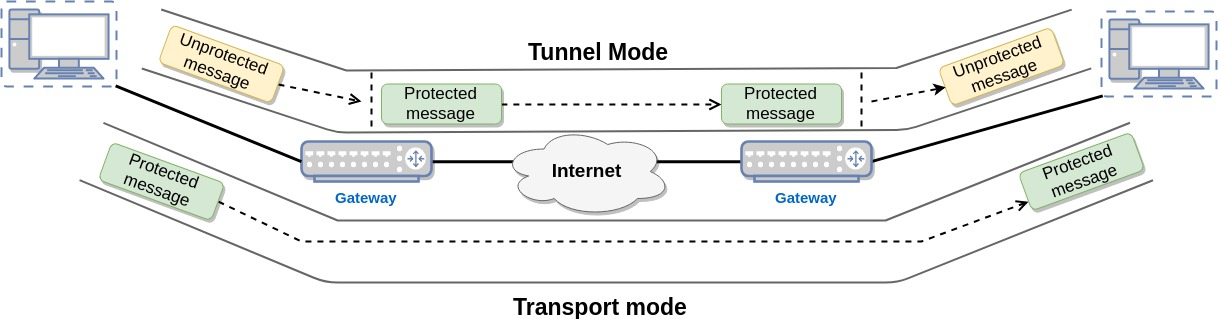
\includegraphics[width=16cm]{figures/IPsec/ipsec_modes.jpg}
 \caption{IPsec communication modes}\label{ipsec_communication_modes}
 \end{figure}

 To provide its security services, \ac{IPsec} use three independent protcols:

 \begin{itemize}
 \setlength{\labelwidth}{10pt}
   \item \ac{AH}: It provides integrity and authentication for the \ac{IP} header and its payload in both tunnel and transport modes and optionally provides protection against replay attacks. However, it does not provide confidentiality. The \ac{IP} header mutable fields (the fields which can change during the transmission) like
   \ac{TTL} are not authenticated.
   \item \ac{ESP}: It provides confidentiality, integrity, and authentication for the \ac{IP} payload in both modes.
   However, it does not provide protection for the \ac{IP} header.
   \item \ac{IKE}: It allows to share an authenticated secret key to be used for encryption, authentication, and integrity checks.
   it uses DH as a key exchange algorithm and RSA for digital signatures.
 \end{itemize}

 As depicted in \autoref{ipsec_protocols}, whether \ac{AH} or \ac{ESP} is adopted, if the tunnel mode is used, when the gateway receives the original \ac{IP} datagram from the sender,
 it encapsulates it into a new \ac{IP} datagram containing a new \ac{IP} address which corresponds to the receiving gateway and then the message is protected. When the transport mode is used the original \ac{IP} datagram is protected by the sender and sent without new \ac{IP} encapsulation.
 \ac{ESP} and \ac{AH} could be used separately or together according to the needed security services.


 \begin{figure}[!htbp]
 \centering
 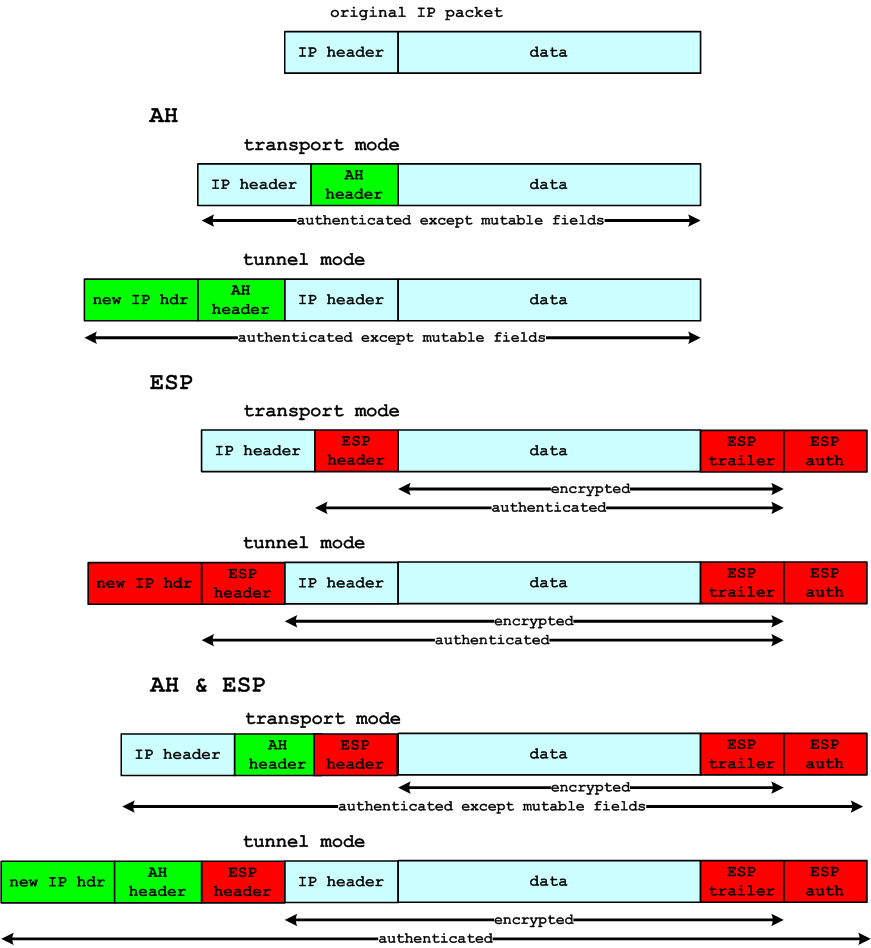
\includegraphics[width=16cm]{figures/IPsec/ipsec_protocols.png}
 \caption{IPsec protocols}\label{ipsec_protocols}
 \end{figure}

\section{Choice of Security Protocol}

We need to take into consideration first that SafetyNETp \ac{RTFN} works on top of \ac{UDP}.
\ac{DTLS} and \ac{TLS} provide the same security services. \ac{TLS} is used for reliable transport protocols whereas DTLS
is for unreliable ones. \ac{IPsec} can be used for securing any type of traffic working on top \ac{IP}.
Therefore our choice is restricted between \ac{DTLS} and \ac{IPsec}.

Automation systems and their real-time operating
systems often are resource constrained and do not include typical security technologies,
and there may not be available computing resources to retrofit these security technologies. \ac{IPsec} tunnel mode
is a solution as the cryptographic operations are performed by the gateways. The end devices send and receive the messages transparently, no additional treatment is needed for them. However, the tunnel mode protects the network only from outside because
messages exchanged on the local network are not secured by the gateway. Hence, we could have serious problems if
an attacker gains access to the local network. \ac{IPsec} transport mode provides end-to-end security and allows to secure the network both
from inside and outside, however, the cryptographic operations are done by the end devices which have constrained resources.
\ac{IPsec} operates at the \ac{IP} layer, it generally must be implemented in the operating
system kernel, either directly compiled in or linked in as a loadable module. This makes \ac{IPsec} fairly inconvenient
to install on non-\ac{IPsec} systems. \ac{AH} and \ac{ESP} are typically implemented in the kernel as part of the \ac{IP} stack, while \ac{IKE}
is implemented as a user daemon. This makes its integration difficult as most of the embedded \ac{IP} stacks do not implement \ac{IPsec}.

\ac{DTLS} provides end-to-end security and like \ac{IPsec}, the cryptographic operations are performed by the end devices.
\ac{DTLS} operates between the transport layer and the application layer. Using DTLS, it is easy to secure an application
 protocol by simply inserting it between the application and the transport layers. \ac{DTLS} is \ac{IP}-stack-independent
which means that it does not include any modification to the underlying \ac{IP} stack and could be used with any \ac{IP} stack implementation,
hence, its integration in embedded \ac{IP} stacks is a lot easier.

Having that Both, \ac{IPsec} and \ac{DTLS} provide the needed security services (confidentiality, integrity, and authentication),
and based on the previous paragraphs, we decide to use DTLS.

\section*{Conclusion}

After going through the necessary concepts needed for our project, in the next chapter, we go through a
brief security analysis and we present the functional and non-functional requirements.

%_____________________________________________________________________________________
%
%       Filename:  chapter3.tex
%
%    Description:  Thesis Template HS Offenburg
%
%
%         Author:  Okba ZOUEGHI, okba.zoueghi@gmail.com
%     Supervisor:  Andreas Walz, Chadlia Jerad
%   Organization:  HS Offenburg, Offenburg, Germany
%
%_____________________________________________________________________________________

\chapter{Requirement Analysis and Specification}

After introducing the basic concepts, we move in this chapter to conduct first a brief security
analysis in which we outline the assets as well as the threats, thereafter, we go through the requirements
analysis in which we cite the functional and the non-functional requirements.
Finally, we present the requirements specification using a use case diagram.

\section{Threat Analysis}

Security is the set of means implemented for minimizing the vulnerabilities of an information
system against accidental and/or intentional threats. Its main goal is to protect the system sensitive elements and
resources from threats according to the needs. Therefore, we need to define as a first step what
are the assets that we will be protecting, as a second step we present the threats related to the scope of our project.

In our project, our goal is to provide an end-to-end security for SafetyNETp RTFN based network, therefore,
the assets we will be protecting are every device in the network which runs SafetyNETp RTFN application.
In today’s SafetyNETp RTFN based networks, data transmission is
performed without any special security measures. The lack of security measures can create unforeseen security threats to the network,
the data, and the resources. In our project, we are interested only with threats with regards to the general security objectives
namely confidentiality, integrity, and authenticity. Any other threats are out of the scope of our project, for instance,
physical attacks, vandalism, theft of equipment, etc.

In the following, we highlight some of the threats that a SafetyNETp network could face because of the lack of
security measures.

\renewcommand{\labelitemi}{$\bullet$}
\begin{itemize}
\item Identity impersonation: To get \textit{cyclic data} about a certain topic, subscribers send \textit{subscribe requests} as broadcast.
Upon receiving \textit{subscribe acknowledgments}, subscribers start consuming \textit{cyclic data} without any verification about the publishers'
identities. Therefore, an untrusted third party can easily impersonate the identity of a device to create and send
its own malicious \textit{cyclic data}. As no authentication mechanism is present, subscribers take decisions about the action to perform
based on malicious and untrusted \textit{cyclic data} which is highly dangerous. Furthermore, an attacker can easily flood a publisher
with a huge number of \textit{subscribe requests} using spoofed IP addresses, hence, overloads the publisher and the bandwidth and eventually can
cause a DoS attack.\\


\item Data tampering: When a \textit{cyclic data} message is received, no integrity checks are performed by the subscriber
and the data is consumed directly. In fact, SafetyNETp RTFN application layer does not provide any mechanism for
verifying messages' integrity. Therefore, with a man in the middle attack, an attacker can easily intercept the messages
being exchanged and modify the \textit{cyclic data} being
sent from a publisher to a subscriber.\\

\item Eavesdropping: The data communicated between two plants in different geographical areas passes through the internet.
SafetyNETp RTFN application layer does not provide any mechanism for protecting confidential data, in fact,
the messages are sent as plaintext. Without encryption, exchanging data through the internet, any third party can
easily have access to highly confidential data.\\
\end{itemize}

To illustrate better, we take a real-life example where SafetyNETp is used and where security is very important.
In fact, SafetyNETp provides a solution for railways automation \cite{pilz_rail_engineering} where SafetyNETp devices control the trains' tracks, the
level crossing protection system as well as functions in and around the trains. Having snow and low temperature could interrupt
the railway's operations, that's why Pilz hand over a heating system to provide the needed temperature. This is implemented by a temperature sensor
and a heater. The heater gets the temperature value from the sensor and takes the decision based on that. \autoref{pilz_railway_heater} shows
the railway after and before that the heater took the decision. With the lack of authenticity, an attacker can send false temperature values
to the heater by impersonating the identity of the sensor. The attacker can keep sending high temperature values that keeps the heater
on an idle state and therefore the railway become unusable. An attacker is able also with a man in the middle attack to change the values being
sent by the sensor. As a result, the heater takes decisions based on unauthenticated or tampered data.
SafetyNETp provides a remote access to the devices for control and diagnostic purposes. Exchanging data through the internet
allow third parties to gain access to confidential data like trains' and railways' states.

\begin{figure}[H]
\centering
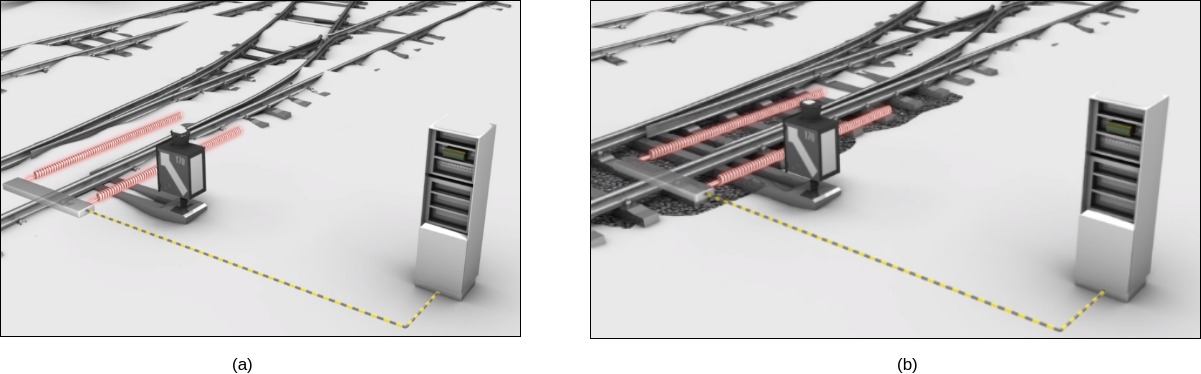
\includegraphics[width=17cm]{figures/requirements/railway_heater.jpg}
\caption[Pilz railway heater system]{Pilz railway heating system\cite{pilz_rail_engineering}}\label{pilz_railway_heater}
\end{figure}






\section{Requirement Analysis}

In this section, we present the functional and the non-functional requirements that our security layer should satisfy.

\subsection{Functional Requirements}

Based on DTLS, our security layer should provide the following requirements:

\renewcommand{\labelitemi}{$\bullet$}
\begin{itemize}
\item Authentication: Recipients of a message can identify their communication partners and can detect
if the sender information has been forged.\\

\item Integrity: Communication partners can detect changes to a message during transmission.\\

\item Confidentiality (Optional): If the messages are confidential, they could be encrypted and only
the authorized devices could be able to decrypt messages and read the content.
\end{itemize}

\subsection{Non-functional Requirements}

Our security layer should respect the following constraints:

\renewcommand{\labelitemi}{$\bullet$}
\begin{itemize}

\item Transparent integration: The security layer should not perform any changes to SafetyNETp application
layer state machine.\\

\item Easily Configurable: Changing the parameters of the security layer should be easy for SafeyNETp developers.\\

\item Time and memory constraints: The security layer needs to keep SafetyNETp cycle time as it is as much as possible
and to optimize memory consumption.\\

\item Maintainability: The security layer needs to be easy to understand and to maintain.


\end{itemize}

\section{Requirement Specification}

In this section, using a use case diagram, we formalize our requirements by illustrating the interaction between the security layer
and our only actor which consists of SafetyNETp application layer.

\begin{figure}[H]
\centering
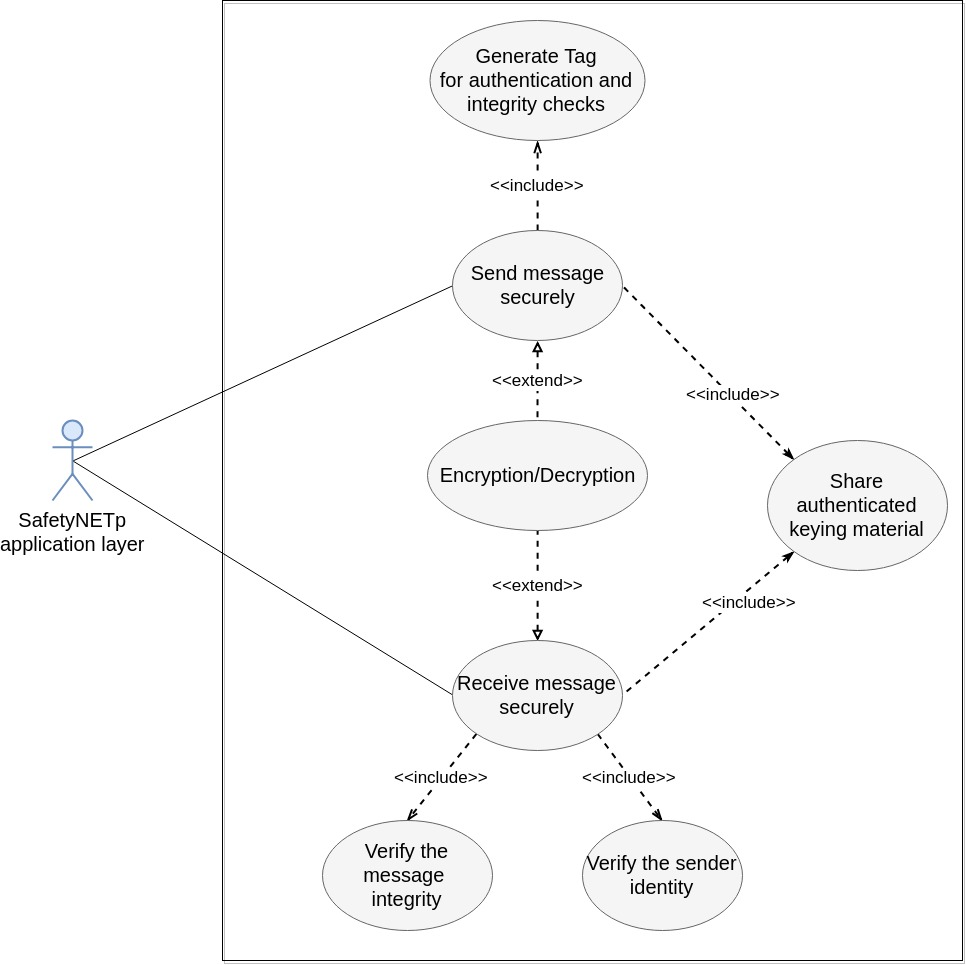
\includegraphics[width=13cm]{figures/requirements/use_case.jpg}
\caption{General use case diagram}\label{general_use_case_diagram}
\end{figure}

As depicted in \autoref{general_use_case_diagram}, our security layer allows SafetyNETp application layer to both, send and receive messages securely.
Indeed, we need first the establishment of shared authenticated keying material. Thereafter, if the operation
is sending, a tag will be generated by our security layer and sent to allow the receiver to authenticate the sender and verify the integrity of
the received message. If the operation is receiving, using the tag, the receiver is able to authenticate the sender and verify the message integrity.
In some application we may don't need confidentiality, therefore, the encryption is optional. In fact, in applications where
confidentiality is not required, sending data without encryption allows reducing significantly the CPU usage.

\section*{Conclusion}

After we set the requirements that our security layer should satisfy, we pass in the next chapter to discuss
the global and the detailed design.

%_____________________________________________________________________________________
%
%       Filename:  chapter4.tex
%
%    Description:  Thesis Template HS Offenburg
%
%
%         Author:  Okba ZOUEGHI, okba.zoueghi@gmail.com
%     Supervisor:  Andreas Walz, Chadlia Jerad
%   Organization:  HS Offenburg, Offenburg, Germany
%
%_____________________________________________________________________________________

\chapter{Design}

% During this chapter, we start by specifying the functional and non-functional requirements
% then pass to

In this chapter, we provide and discuss the candidate solutions for integrating the DTLS
protocol within SafetyNETp RTFN communication model. Our security layer DTLS-based design is
discussed in two parts. In the first part, we see the global design in which we discuss
the handshake timing, DTLS and SafetyNETp role mapping as well as the secure channel creation.
The second part is the detailed design, in this section, we go deeper into the solutions to
see the security layer positioning, how the outgoing and incoming message are treated,
the frame layout as well as several other details.

\section{Global Design}

As we mentioned before it is easy to provide a secure channel for an application layer
protocol by inserting DTLS or TLS (based on the underlying transport layer) between the application
layer and the transport layer. For instance, \ac{HTTPS} is a secure version
of \ac{HTTP}, this security is provided by inserting TLS between TCP and \ac{HTTP}. This is made easy due to the
fact that \ac{HTTP} and TLS follow both the Client/Server communication model.

Unlike \ac{HTTP} and similar protocols, providing a DTLS-based security layer for SafetyNETp is not as simple as it seems.
In fact, SafetyNETp is based on Publish/Subscribe communication model, on the other hand, DTLS is designed for
Client/Server based applications. Hence, we need a solution which allows mapping and adapting
DTLS to SafetyNETp. Furthermore, an important question could be asked: in which step of SafetyNETp
communication the handshake should be established?

In this section, we see when the DTLS handshake is established, how to manage
mapping the roles for the different communication model and we present how a secure channel
is provided.

\subsection{When To Establish The Handshake?}


As shown in \autoref{when_to_establish_the_handshake}
there are three possible alternatives. Establish the handshake before sending a \textit{subscribe request}, after sending
a \textit{subscribe request} but before receiving an acknowledgment, and the last alternative after receiving an
acknowledgment. These cases correspond to the device which takes the subscriber role. Regarding
the publisher, there are two alternatives, whether after or before sending a \textit{subscribe acknowledgment}.

\begin{figure}[!htbp]
\centering
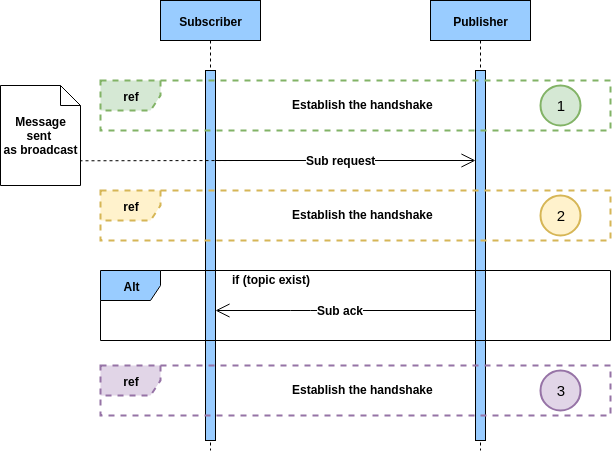
\includegraphics[width=12cm,height=9cm]{figures/design/when_to_establish_the_handshake.png}
\caption{Possible cases of handshake establishement}\label{when_to_establish_the_handshake}
\end{figure}

% As we mentioned before publishers and subscribers don't know each other in advance. Therefore
% the subscriber could not establish the handshake in the first and the second case because the publisher
% which is the second handshake end-point is unknown at this level. For the first two cases, the solution is to establish
% the handshake with all the devices. For that, the subscriber needs to know the possible ranges of IP addresses
% that can be used in the network. the advantage of this solution is that the first subscription
% process will be performed through the secure channel created after the handshake was established.
% However, this solution is not efficient in term of memory and bandwidth usage, in term of startup time
% and in term of flexibility.  For each handshake, memory resources need to be allocated which is memory
% waste because not all the channels will be used by the subscriber. To perform the handshake, if we assume
% for example that the subscriber has a client role, it sends Client Hello message to all the IP addresses
% existing in the used IP ranges. Therefore messages will be sent also to unused IP addresses which is
% bandwidth waste. The startup time will increase if the number of devices is important. Regarding the flexibility,
% if a new IP addresses range is used in the network, the devices need to be reconfigured.
%
%
% Regarding the third case, after that the subscriber receives a \textit{subscribe acknowledgment} from the publisher,
% at this level, the subscriber knows the second handshake end-point and the handshake could be established.
% The disadvantage of the previous solution is not present here. Only necessary channels will be created
% which optimizes the memory and the bandwidth usage and reduces the startup time. Furthermore,
% no information needed about the IP addresses ranges which allow more flexibility. Unfortunately,
% the first subscription process will not be authenticated in addition the publisher starts
% sending \textit{cyclic data} to the subscriber after sending the \textit{subscribe acknowledgment} which presents an issue.
% In fact the \textit{cyclic data} will be sent while the handshake is being established, however, the
% identity of the second end-point is not verified. Hence \textit{cyclic data} will be sent to untrusted devices.
%
% In the third case, the subscriber and the publisher know each other addresses which solves
% the problems present in the first and the second case. Comparing these alternatives, the third is better in term of
% memory, bandwidth, flexibility and startup time. Therefore we choose to establish the handshake after the first subscription process.
% We see in the next sections how we solve the authentication issue for the first subscription
% as well as sending \textit{cyclic data} to untrusted devices.

As we mentioned before publishers and subscribers don't know each other in advance. Therefore
the subscriber could not establish the handshake in the first and the second cases because the publisher
which is the second handshake end-point is unknown at this time. For the first two cases, the solution is to establish
the handshake with all the devices. The handshakes establishment is triggered by the devices' startup, therefore,
it is not possible to add a new device to the network at runtime. Assuming that we have a network of RTFN devices, at startup time,
all the devices will establish the handshake with each other and they start exchanging data. If we add a new device after this phase,
no handshake will be established with it as the handshakes phase has already finished, hence, the new device will not be able
to communicate securely. To be able to add a new device to the network, the devices should be restarted.
Furthermore, this solution is not efficient in term of memory usage and startup time.
For each handshake, memory resources need to be allocated which is memory
waste because not all the channels will be used by the subscriber.
Besides, the startup time will increase if the number of devices is important.
This method introduces another inconvenient, a session between a publisher and a subscriber should remain always open
even if no communication is needed. In fact, once the session is closed, they could not establish a new session
as it is triggered by the startup. Letting unnecessary sessions open leads to memory waste.


Regarding the third case, after that the subscriber receives a \textit{subscribe acknowledgment} from the publisher,
at this level, the subscriber knows the second handshake end-point and the handshake could be established.
The disadvantages of the previous solution are not present here. Only necessary channels will be created
which optimizes the memory usage and reduces the startup time. In addition unlike the previous cases,
unnecessary sessions could be closed as the handshake is triggered by the subscription process (more details about sessions closing are
given in the next sections). Unfortunately, our security layer
needs in this case to inspect the application layer header in order to take the decision.
Furthermore, the publisher starts
sending \textit{cyclic data} to the subscriber after sending the \textit{subscribe acknowledgment} which presents an issue.
In fact the \textit{cyclic data} will be sent while the handshake is being established, however, the
identity of the second end-point is not verified. Hence \textit{cyclic data} could be sent to untrusted devices.

The \autoref{alternatives_comparison} shows the main differences between the cited alternatives.

\begin{table}[H]
  \centering
    \begin{tabular}{|l|l|l|}
      \hline
      & First and second cases & Third case \\
      \hline
      Memory usage & more & less \\
      \hline
      Startup time & more & less \\
      \hline
      Message inspection & no & yes \\
      \hline
      Flexibility & no & yes \\
      \hline
      Close unnecessary sessions & no & yes \\
      \hline
      Cylic data sent while & &\\
      establishing the handshake & no & yes \\
      \hline
  \end{tabular}
  \caption{Alternatives comparison}\label{alternatives_comparison}
\end{table}


In the third case, the subscriber and the publisher know each other addresses which solves the problems present in the first and the second cases. Comparing these alternatives, the third is better in term of
flexibility, memory usage, and startup time. Therefore we choose to establish the handshake after the first subscription process.
We see in the next sections how to deal with the \textit{cyclic data} sent while the handshake is being established.


\subsection{SafetyNETp and DTLS Role Mapping}

After choosing when to establish the handshake, an important question could be asked.
How to map DTLS roles (client/server) with SafetyNETp roles (publisher/subscriber)?
The intuitive solution is that the subscriber takes the role of the client and the publisher
takes the role of the server. After sending the \textit{subscribe acknowledgment}, the publisher
activates its servers and waits for a Client Hello message. After receiving the subscribe
acknowledgment the subscriber takes the client role and sends a Client Hello to the publisher
which has already activated its server and which is ready to establish the handshake. Once the handshake
has finished successfully, the publisher can send \textit{cyclic data} securely through the created secure channel.


Unfortunately, if we consider that two SafetyNETp devices could have a mutual subscription,
an issue is presented. As shown in \autoref{simultaneous_mutual_subsribtion}, the devices A and B subscribe mutually to each other in parallel
at the same time. As discussed in the previous section the event which triggers the
handshake establishment is the subscription process. With the method presented above, having simultaneous
subscription will lead to create two channels between A and B. We will end up having a channel for each relation of
(publisher,subscriber). In the case shown in \autoref{simultaneous_mutual_subsribtion} we have two relations, the relation (A,B), in which A
is the publisher and B is the subscriber and the (B,A) relation which is the opposite. Therefore two
separate channels will be created between A and B whereas one single channel is sufficient.

Creating more than one channel for the same couple leads to more memory usage that's why
we need a mechanism to avoid duplicated channels. After that both of A and B had sent
the \textit{subscribe acknowledgment}, they know each other's IP addresses. Based on the IP addresses,
each device can choose a distinct DTLS role. The device which has the greater IP address
takes the server role, the other device takes the client role.
Therefore, we choose to use IP addresses as a criterion to map DTLS and SafetyNETp roles. Other alternatives
than the IP addresses could be used like MAC addresses for example. What is important is to make the choice and break the conflict
to avoid duplicated channels which could be achieved using this method.

\begin{figure}[H]
\centering
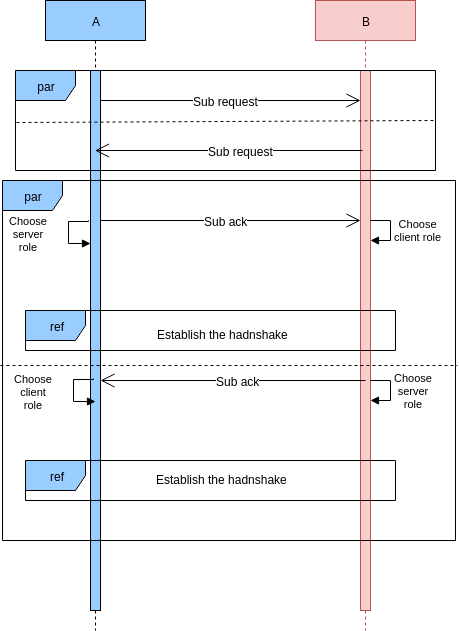
\includegraphics[width=9cm,height=9cm]{figures/design/mutual_subsribtion.png}
\caption{Simultaneous mutual subscription}\label{simultaneous_mutual_subsribtion}
\end{figure}

\subsection{Secure Communication}

As a first step, we discussed when to establish the handshake, as a second step
we defined a mechanism to map the client/server role with the publisher/subscriber role.
As mentioned before, if the handshake is established after the subscription process,
the publisher starts sending \textit{cyclic data} while the handshake is being established.
This can lead to send \textit{cyclic data} to unauthorized devices as the data is sent before finishing the handshake.
In this section, as a next step, we take into consideration this issue and then we see a nominal case of a secure communication between two devices

\textit{Cyclic data} messages are very important that's why they should not be sent or received from
an untrusted device. While the handshake is being established, for the publisher,
the identity of the subscriber is not verified yet. As mentioned in the non-functional
requirements, our security layer should not introduce any changes to SafetyNETp state machine, therefore, two decisions could be taken,
whether to drop or to store the \textit{cyclic data} until finishing the handshake. If the \textit{cyclic data}
is stored, once the handshake is finished and the identity is verified, nothing is lost and
the \textit{cyclic data} could be sent securely through the secure channel. However, storing the cyclic
data can eventually cause a DoS attack. In fact, an attacker could send a huge number
of \textit{subscribe request} to a publisher with spoofed IP addresses. The publisher will send
a \textit{subscribe acknowledgment} for each received request and then start storing the \textit{cyclic data}
until verifying the identities. Eventually, the identities will not be verified but the publisher
memory will become saturated and the publisher will be out of service. This is the first
reason for which the \textit{cyclic data} should not be stored, furthermore, the \textit{cyclic data} represent
information about a certain topic and based on its content subscribers take actions.
Having old information about a topic can cause serious problems, that's why we choose to drop
\textit{cyclic data} while establishing the handshake.

\begin{figure}[!htbp]
\centering
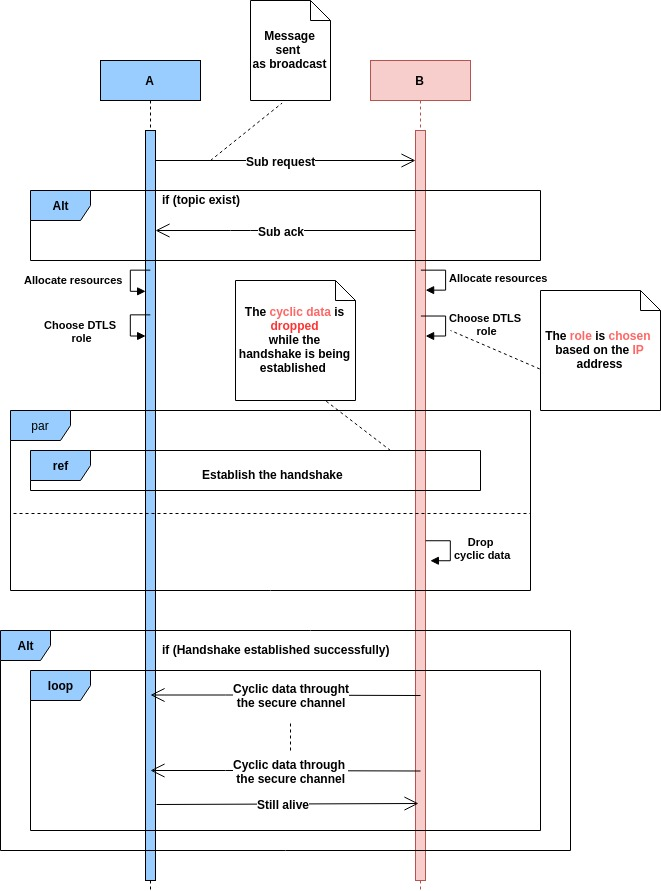
\includegraphics[width=11cm,height=15cm]{figures/design/nominal_case_for_secure_communication.jpg}
\caption{Nominal case of a secure communication}\label{nominal_case_for_secure_communication}
\end{figure}



The \autoref{nominal_case_for_secure_communication} illustrates a nominal case of a secure communication between two SafetyNETp devices.
Once the subscription process is done, both of the devices allocate the necessary memory needed for the
secure channel and then they choose DTLS roles based on their IP addresses. The handshake then starts, and the \textit{cyclic data}
is dropped. Once the handshake is finished successfully, sending the \textit{cyclic data} is resumed to be sent
through the secure channel.

\section{Detailed Design}

\subsection{Security Layer Positioning}

In this section, we see the positioning of the security layer and SafetyNETp in the TCP/IP model
and we discuss according to the messages' types whether a message should be sent through the security layer
or not.

As illustrated in \autoref{the_security_layer_and_safetynetp_in_tcp_ip_model}, the security layer is between UDP (transport layer) and SafetyNETp (application layer).
Sending a SafetyNETp application message can follow two paths, whether to be packed directly into a UDP datagram
or packed into our security layer frame and then into UDP. One can ask why would we enable SafetyNETp to skip the security layer
and use directly UDP. As we saw before in order to switch to a secure communication, the DTLS handshake need to be established.
The trigger of the handshake establishment is the first subscription process that's why the first subscription messages are sent
unprotected because at this level no secure channel exists.

\begin{figure}[H]
\centering
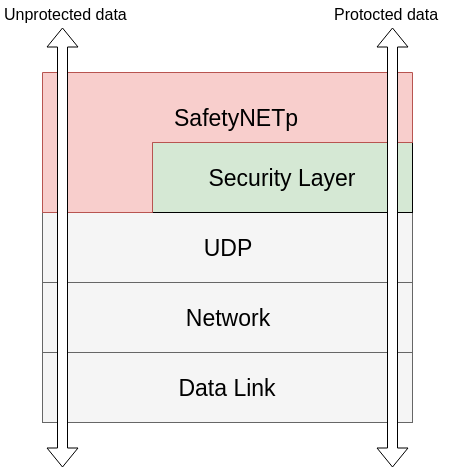
\includegraphics[height=7cm]{figures/design/the_security_layer_and_safetynetp_in_tcp_ip_model.png}
\caption{The security layer and SafetyNETp in TCP/IP model}\label{the_security_layer_and_safetynetp_in_tcp_ip_model}
\end{figure}

Once The handshake is established, a secure channel is provided and data could be exchanged securely but what are the
messages that should be sent through the secure channel? Do all of them should be sent securely?
Regarding \textit{subscribe requests} and \textit{acknowledgments} they obviously need to be sent securely, otherwise, a fake
\textit{subscribe request} could be sent and unnecessary data will be exchanged which leads to more CPU processing in both sides
(publisher and subscriber) and more bandwidth usage.
Actually, an attacker could use the fact that the subscription messages are unprotected. Being unprotected means that no integrity checks are
performed, therefore, if an attacker modifies the content of a message, the modification will not be detected.
A possible attack is shown in \autoref{man_in_the_middle_attack_exploiting_unprotected_subsribtion}, in this example, the attacker could modify the content of the packets with
a man in the middle attack. When the subscriber sends a \textit{subscribe request} for a topic X, the attacker
intercepts the messages and modifies it by changing the topic to Y. When the publisher receives the message it
sends back an acknowledgment and starts sending \textit{cyclic data} for topic Y which is not needed by the subscriber.
Moreover, an attacker could entirely forge and send fake \textit{subscribe requests} and, therefore, the bandwidth could be saturated.
The \textit{subscribe requests} are sent as broadcast to all the devices present on the network as the topic owner is
unknown in advance. Each secure channel corresponds to a couple of a publisher and a subscriber and there is no
secure channel shared between all the devices. Therefore, \textit{subscribe request} messages could not be sent securely as broadcast.
In order to avoid the previous problem, alongside sending the \textit{subscribe requests} as broadcast, the subscriber also
sends the same \textit{subscribe requests} as unicast and secured to the publishers with which it has an available secure channel.
When a publisher receives a \textit{subscribe request} as broadcast and unprotected from a subscriber, if it has an available
secure channel, the publisher ignore the subscribe request. If the publisher has no channel, it goes through the handshake establishment.
Hence, the publisher could avoid sending \textit{cyclic data} when receiving a tampered or a forged subscribe request.

\begin{figure}[H]
\centering
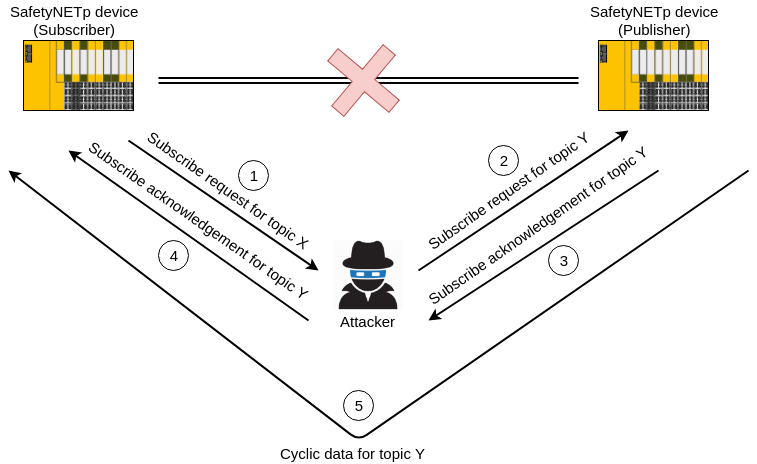
\includegraphics[height=7.5cm]{figures/design/man_in_the_middle_attack.png}
\caption{Man in the middle attack exploiting unprotected subscription}\label{man_in_the_middle_attack_exploiting_unprotected_subsribtion}
\end{figure}

As the rest of the messages are sent as unicast, they could be secured easily unlike the \textit{subscribe request} message.
The \textit{unsubscribe} and \textit{unpublished} messages could cause
issues if they are unprotected. In fact, an attacker could send a fake \textit{unsubscribe request} to a publisher
which will stop sending \textit{cyclic data} upon receiving the message. The last message type is the \textit{still alive} message,
as we discussed before it is used by the subscriber to inform the publisher that it is still alive. Therefore,
if it is sent unprotected, when a subscriber reboots for example, an attacker can send \textit{still alive} messages
to the list of publishers communicating with the subscriber. Hence they will not detect that the subscriber is down.
To conclude after analyzing the situation for each message type, once the handshake is established all
the messages should be sent through the secure channel.

\subsection{Flowcharts for Outgoing Messages}

In any SafetyNETp device using our security layer, whether the device is a publisher or a subscriber,
each outgoing message should follow the flowchart in \autoref{outgoing_messages_flowtchart}.

Let's take the example of two SafetyNETp devices, a subscriber
and a publisher respectively A and B. Initially, before starting the communication, no secure channel is available.
The communication starts when A sends a \textit{subscribe request} to B. The \textit{subscribe requests} are sent
unprotected as broadcast following the Path 4 and as no secure channel exists, no \textit{subscribe request} will be sent protected at this level.

Upon receiving the \textit{subscribe request}, like A, B will verify first if there is a secure channel for A.
Obviously, no secure channel exists, therefore, the \textit{subscribe acknowledgment} is sent unprotected and Path 1 is followed.
After sending the \textit{subscribe acknowledgment}, B will allocate the necessary resources and launch the handshake.
If the handshake is launched as a server, B will just wait for Client Hello messages coming from A, if it is
launched as a client, B will start sending Client Hello messages to A. Following the \textit{subscribe acknowledgment},
B will start sending \textit{cyclic data}. In this level, the handshake is being established, which means the identity of A
is not verified yet. The \textit{cyclic data} should be dropped, hence, Path 2 is followed. While establishing the handshake,
each \textit{cyclic data} message will follow Path 2 until it is finished. Once the first handshake is
established (we will have more than one handshake, more
details are given this in the next sections), every message is switched to be sent through the secure
channel. All the messages except \textit{subscribe requests} are sent following path 5. After that the handshake is established,
following the path 4, the \textit{subscribe requests} are sent unprotected as broadcast and secured as unicast through all the available channels.
In this case, If A performs another subscription after that the handshake is established, B will receive two subscribe requests
for the same topic, one as unicast through the security layer, and the other original unprotected broadcast subscribe request.
Obviously B, ignore the one sent as broadcast and process only the secured request. As we mentioned before,
sending \textit{subscribe requests} secured as unicast, enables the publisher to avoid responding for tampered and forged subscribe requests.

The path 3 shows how messages other than \textit{subscribe requests} and \textit{cyclic data} are sent before and while establishing the handshake.

\begin{figure}[p]
\centering
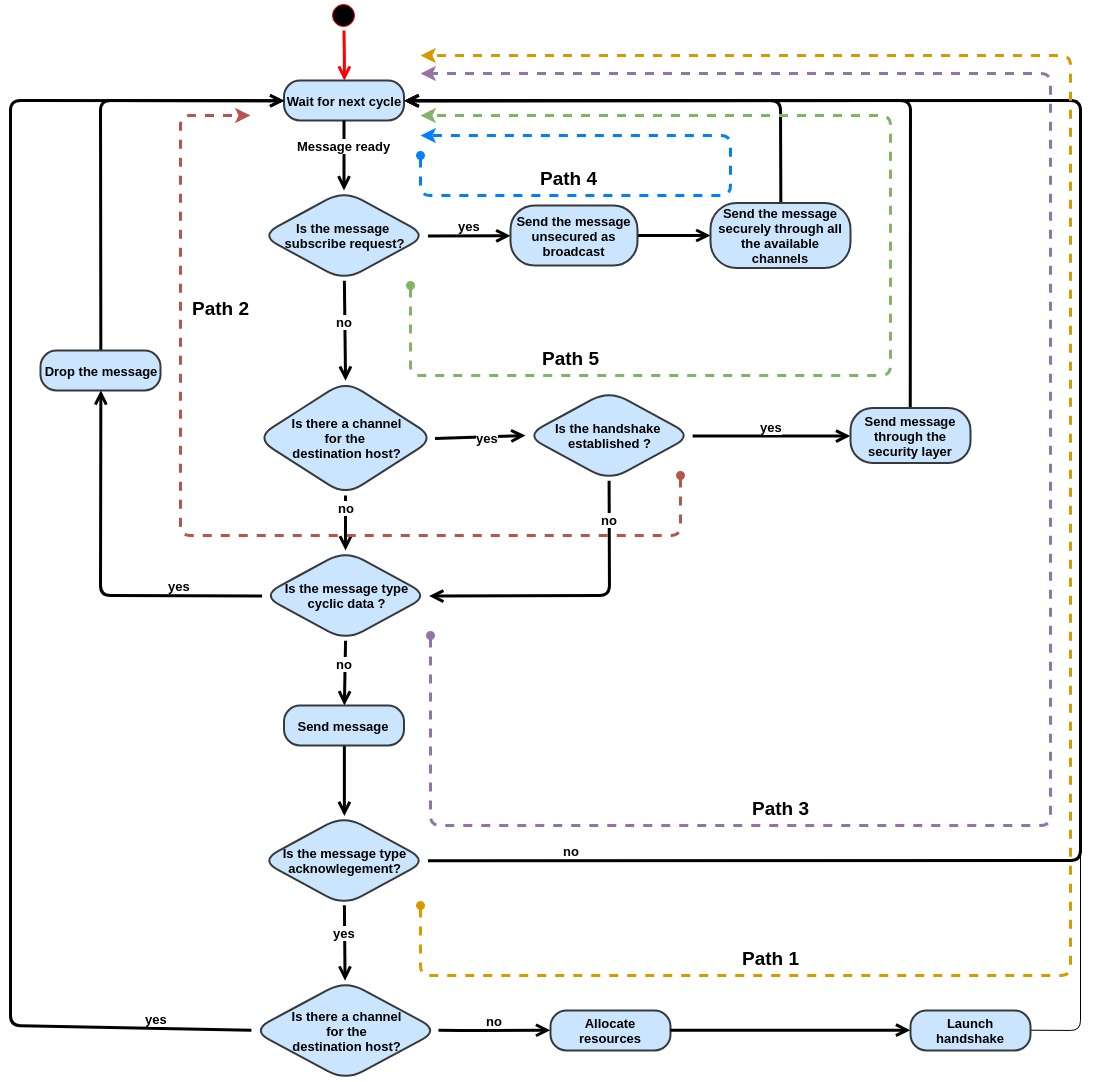
\includegraphics[height=16cm]{figures/design/outgoing_messages_flowtchart.jpg}
\caption{Flowchart for outgoing messages}\label{outgoing_messages_flowtchart}
\end{figure}

\newpage
\subsection{Flowchart for Incoming Messages}

Following the flowchart in \autoref{outgoing_messages_flowtchart} we ensure a secure encrypted and authenticated
communication in which messages are sent only to authorized devices, However, this flowchart does not include
the flow for received messages. The flowchart in \autoref{incoming_messages_flowtchart} illustrates how each incoming message is treated.

When \textit{cyclic data} is received and no secure channel is available, the message is dropped as shown in Path 1.
If we assume that we have a subscriber and a publisher respectively A and B, after sending a \textit{subscribe request}, A
will receive the first \textit{subscribe acknowledgment}. Upon receiving it, as no channel exists, A will allocate
the necessary resources and launch the handshake (Path 2). Meanwhile, if a \textit{cyclic data} message is received it
will be dropped as the identity of B is not verified yet (Path 1).

Once the first handshake is established, A and B will switch to
communicate via the secure channel. When a message is received the identity of the sender as well as
the message integrity will be verified. If the message is verified correctly, it will be decrypted and passed to SafetyNETp
application layer to get processed (Path 3). If the message is not verified it will be dropped (Path 4).

When an attacker impersonates the identity of B for example and sends a \textit{cyclic data} message to A,
if no secure channel is available, the message will be dropped (Path 1). After the handshake is established, if the attacker
finds a way to modify messages, the integrity checks will fail and the message will be dropped (Path 4).

\begin{figure}[p]
\centering
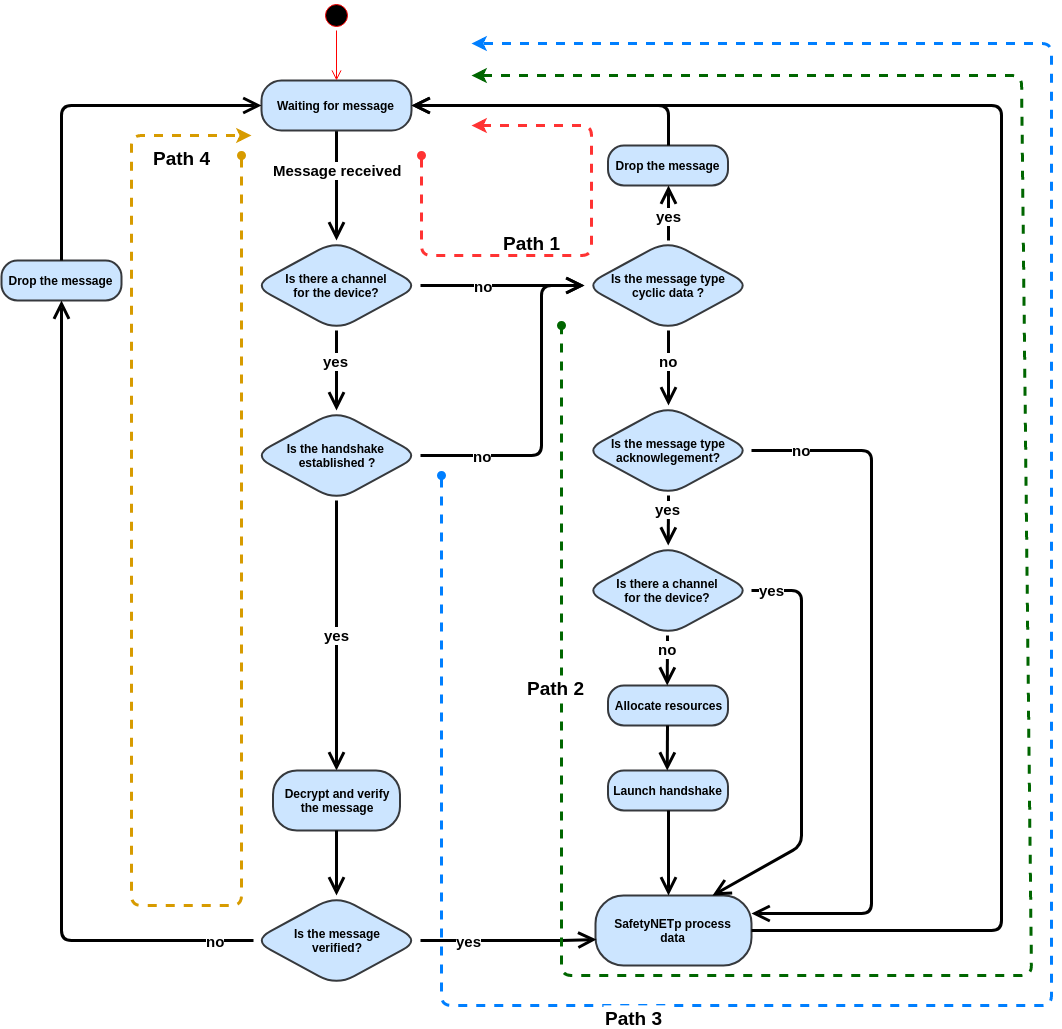
\includegraphics[height=16cm]{figures/design/incoming_messages_flowtchart.jpg}
\caption{Flowchart for incoming messages}\label{incoming_messages_flowtchart}
\end{figure}
\newpage

\subsection{First Subscription Vulnerability}

Triggered by the first handshake process, the devices establish the DTLS handshake and start exchanging
data securely. The trigger for establishing the handshake could not be secured as no secure channel exists
before establishing the handshake. Therefore we are obliged to perform the first subscription unprotected as it is the trigger.
We already mentioned the issues of sending unprotected subscribe requests. Fake \textit{subscribe requests} could be sent
which results on exchanging unnecessary data in the network. We already proposed a solution for securing subscribe requests
after the secure channel is provided, however, we did not discuss the first subscription issue.

When the system starts up, before any message is exchanged, an attacker could easily impersonate the identity
of a device and send a \textit{subscribe request} with its identity. The device which has the topic will send back a
subscribe acknowledgment as response and both devices will establish the handshake. As the first subscription is
forged by the attacker, the \textit{cyclic data} sent by the publisher is not needed by the subscriber.

In order to avoid receiving the unnecessary cyclic data, we propose two solutions.
After that the handshake is established, we reset the application state of the two parts the publisher and the subscriber.
By resetting the application state, both the publisher and the subscriber forget about the previous subscriptions
and they perform the subscription process another time. Therefore, if the first subscription is fake, by resetting the
application state, no \textit{cyclic data} for the fake subscription will be sent and all the new subscription could be performed
securely using the available channel. In fact, this solution could not be applied currently, as SafetyNETp does not provide
an API for resetting the application. However, The solution is interesting and we could ask SafetyNETp developers for such API to solve the problem.

The second solution consists of changing the handshake timing previously discussed and perform the handshake
at the second position shown in \autoref{when_to_establish_the_handshake}. In this case, when a \textit{subscribe request} is
received, our security layer don't pass the message to SafetyNETp to be processed. Because if the topic exists
the device will send a \textit{subscribe acknowledgment} and start sending \textit{cyclic data} which could be unnecessary as
the subscription is not protected. Not passing the \textit{subscribe request} to SafeyNETp allows avoiding this issue.
The device which sends a \textit{subscribe request} activates a server and the receiving device after verifying that the topic exists,
takes the client role and start establishing the handshake with the subscriber. Using this method no subscribe acknowledgment
is sent before establishing the handshake, therefore, no \textit{cyclic data} is sent. After finishing the handshake, our security
layer let SafetyNETp process \textit{subscribe requests} and all the message could be exchanged securely. The problem with this
method is that our security layer is not able to know whether a topic exists or not without letting SafetyNETp process
subscribe requests. In fact, for our security layer, the indicator for the topic existence is the subscribe acknowledgment.
It is not possible to detect whether a topic exists or not without seeing a subscribe acknowledgment. Therefore to make
this possible, SafetyNETp developers need to provide a function which returns whether a topic exists having a subscribe
request as input.

To conclude, the first subscription process is currently performed without protection and the problem
could be solved using one of the cited solutions if SafetyNETp developers could provide the needed APIs.


\subsection{Keying Materials Renewal}

Cryptology is a mathematical science which contains two branches, cryptography, and cryptanalysis.
The main goal of cryptography is to ensure data confidentiality by encrypting an input message called
plaintext to obtain an encrypted output called ciphertext. The obtained ciphertext is unreadable and it can
be decrypted only by parts that have the secret key used for encryption. However, the cryptanalysis
goal is to gain as much information as possible about the original unencrypted data. Cryptanalysis
can lead to decrypt ciphertexts without having the secret key and much worse it can even lead to figure it out. This achieved by several technics, for example, analyzing a huge number of ciphertexts.
This technic is called cryptanalysis with ciphertext-only, which mean that the attacker knows only ciphertexts \cite{Cryptology}.

Our security layer provides authentication, confidentiality, and integrity. These three services rely on keeping the keying
material being used secret. In SafetyNETp networks, using our security layer, publishers send each cycle
encrypted \textit{cyclic data} messages to its subscribers. An untrusted third party can easily obtain a huge number of
encrypted messages which allows him to perform cryptanalysis studies in order to break the encryption.
If the keying materials are compromised, encrypted messages can be decrypted by an attacker, the messages
can be modified without detecting the modification, an attacker will be able to impersonate
the identity of a device legitimately.

The cryptanalysis relies on studying the encrypted traffic which needs a huge amount of encrypted message
and another important factor which is time. To avoid this kind of attacks, we can simply renew
the keying materials by running a new handshake every period of time.
This period should be defined based on how much time an attacker needs to be able to break the encryption.
Once the period is defined, each two communicating devices run a new handshake upon the expiry of the period.
\autoref{keying_materials_renewal} illustrates how keying material renewal is performed. After that the first handshake has been
established, a timeout is set and \textit{cyclic data} is sent using the first provided keying material or in other words the first DTLS context.
Upon the timeout expiry, a new handshake is established in parallel while sending \textit{cyclic data}.
When the new handshake is established, we can choose whether to switch directly to use the new DTLS context
or to wait for a period of time before switching like shown the figure. At each handshake, the timer is reset
and upon its expiry, a new handshake is established and therefore we can minimize the possibility of cryptanalysis attacks.

\begin{figure}[H]
\centering
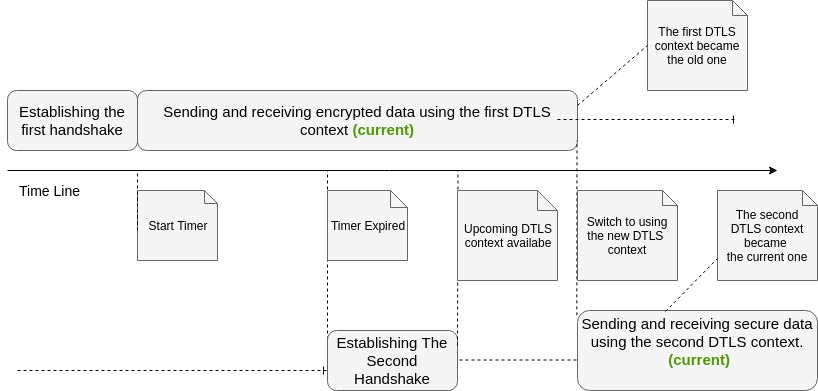
\includegraphics[height=7cm]{figures/design/keying_materials_renewal.jpg}
\caption{Keying Materials Renewal}\label{keying_materials_renewal}
\end{figure}

\subsection{Session Closing}

When no more data need to be exchanged between two devices, the session should be closed and the allocated resources
for the handshake establishment and keying materials should be freed. A session could be closed for several reasons.

First, the subscriber could unsubscribe from all the topics received from a certain publisher, therefore, there will be no more
data published to the subscriber. Hence the secure channel is not needed anymore. At this level, the session can be closed and
the resources can be liberated. In each device, we need to keep track of the topics being used and once no topic is being communicated
the session should be closed. In each Publisher/Subscriber relation, the topics are counted as follows. The subscriber increments
the number of topics being used each time it receives a \textit{subscribe acknowledgment} from the publisher. The subscriber decrements the number
if it receives an \textit{unpublished} message from the publisher or after having sent an \textit{unsubscribe request}. The publisher applies
the same principle, it increments the number after sending a \textit{subscribe acknowledgment} and decrements the number if it receives
an \textit{unsubscribe request} or after sending an \textit{unpublished} message. In every device when the number of topics being used for a session is equal to
zero, the session will be closed. This works fine if we assume that messages are sent reliably, however, if we consider using unreliable
transport we will have issues. Assuming we have a subscriber and a publisher and the subscriber is subscribed for just one single topic,
the number of topics being used on both sides is equal to one. If the subscriber sends an \textit{unsubscribe request} to the publisher and the message is lost,
the subscriber decrements the number of topics being used to become zero which is not the case for the publisher (the message is lost).
In this case, we end up having different numbers on each side and only the subscriber closes the session. Alongside counting the topics,
we add another condition to avoid this desynchronization. A session should be closed if two conditions are satisfied.
For the subscriber, the number of topics being used should be equal to zero and in addition, no \textit{cyclic data} is received. In fact, if the
subscriber still receives \textit{cyclic data} means that there has been a packet loss. Hence the subscriber can resend the \textit{unsubscribe request} until the publisher
stops sending \textit{cyclic data}. For the publisher case, the session should be closed, like the subscriber, if the number of topics
being used is equal to zero and if no \textit{still alive} messages are being received.
% In fact, if the publisher sends an \textit{unpublished}
% message for the last topic and the subscriber is still sending \textit{still alive} messages means that the \textit{unpublished} message is lost and hence it could retransmit the message.

The second case for which a session should be closed is that one of both sides is not working anymore (the devices crashes
or reboots for example). After finishing subscription process, \textit{still alive} messages are sent periodically by the subscriber
to the publisher, hence, if the publisher does not receive \textit{still alive} messages for a well-defined timeout (defined by SafetyNETp application layer),
it considers that the subscriber is down. When the \textit{still alive} message timeout expires, the session should be closed.
Regarding the subscriber, it considers that the publisher is down if it does not receive \textit{cyclic data} messages for also a well-defined timeout (defined by SafetyNETp application layer).
When the timeout expires, the subscriber should close the session.

The last case is when performing a handshake. Whether it is the first handshake or a handshake for session renewal,
if the handshake fails, the session should be closed.

We can have the situation where a publisher and a subscriber have just closed their session
and the subscriber decides to get subscribed another time. As the session was closed, they
need to re-establish the handshake in order to communicate. To avoid this situation, if no
communication is needed between the publisher and the subscriber, the session will not be closed
immediately. Instead, a timeout will be set and the session will be closed when the timeout expires.
This allows more flexibility. While the timeout is not expired,
the session will still open and could be used for a new communication. Hence, no need for a new handshake.

\subsection{Frame Layout}

After that the handshake is established SafetyNETp messages are no more sent as plaintext, instead, they
are sent encrypted and encapsulated into DTLS frames. In order to minimize the possibility of cryptanalysis attacks,
we decided to run a new handshake each a well defined period to renew the keying materials being used.
Due to reordering, it is still possible to receive DTLS frames encrypted by the old keying material
from the previous handshake. Therefore, we are not able to know whether a DTLS frame is encrypted
using the new or the old keying material. Hence the receiving device will not be able to decrypt
and verify messages.

In order to solve this issue, our solution is to add additional information to the message to indicate which keying material was
used for encryption. In fact, this consists of adding a one-byte field before the DTLS frame. This field is incremented each
time the handshake is established. We call this field channel id and according to its value, the receiving device could decide
which keying material to use to decrypt and verify the message.


% The first solution consists of using the DTLS epoch. In fact, the epoch is a one-byte integer field in DTLS frame header.
% After each established handshake, DTLS increments the epoch field to indicate that the keying material
% being used had been renewed. Therefore, the receiving devices will be able to know which keying material
% was used based on the epoch field. In DTLS version 1.2, the epoch value starts from zero and at
% each new handshake, it is incremented. Unfortunately, relying on a DTLS header field means that
% our security will be dependent on the DTLS header format. This dependency can cause a problem in the future
% if new versions of DTLS modifies the header format or how a field is being used. That's why we should use DTLS
% as a black box to avoid any dependency. Hence, if the DTLS header changes, nothing will affect our security
% layer and the design will remain the same. Furthermore, the epoch field is already used differently in DTLS version 1.3 \cite{draftTLSv1.3}
% which still being developed. In version 1.3 the epoch field starts from four instead of zero.

% The second solution is to add additional information in the message to indicate which keying material was
% used for encryption. In fact, this consists of adding a one-byte field before the DTLS frame. This field is incremented each time the handshake is established. We call
% this channel id and according to its value, the receiving device could decide which keying material to use
% to decrypt and verify the message.

% Comparing the two solutions, the second lead to more bandwidth usage by adding additional information into
% the message whereas the first does not include any additional information. However, using the first
% solution creates a dependency between our security layer's design and DTLS's design whereas the second
% solution does not. Hence, the security layer will not be affected by changing the DTLS design in this case.
% Therefore we use the second solution.

\autoref{security_layer_frame_layoutl} shows the security layer frame layout. The first byte indicates that the message is a secured
frame, the second byte is channel id which indicates which keying material was used for encryption. The rest
of the message is the encrypted DTLS frame which encapsulates SafetyNETp application layer message.

\begin{figure}[H]
\centering
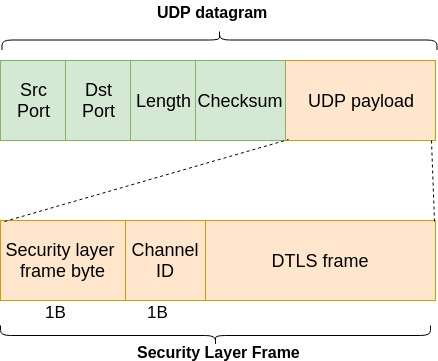
\includegraphics[height=6.5cm]{figures/design/Security_layer_frame_layout.jpg}
\caption{The security layer frame layout}\label{security_layer_frame_layoutl}
\end{figure}

\section*{Conclusion}

Throughout this chapter, we presented the global and the detailed design where we introduced
the existing problems, we provided the candidate alternatives and chose the solutions we judge suitable
for our case.

%_____________________________________________________________________________________
%
%       Filename:  chapter5.tex
%
%    Description:  Thesis Template HS Offenburg
%
%
%         Author:  Okba ZOUEGHI, okba.zoueghi@gmail.com
%     Supervisor:  Andreas Walz, Chadlia Jerad
%   Organization:  HS Offenburg, Offenburg, Germany
%
%_____________________________________________________________________________________

\chapter{Realization}

After designing our security layer, we move in this chapter to see the realization.
We begin by presenting the software and the hardware environments, we move then to present how we implemented
our design, and finally go through testing the implementation.

\section{Work Environment}

For realizing our project, we used a specific hardware
environment as well as a software environment detailed in this section.

\subsection{Software Environment}

In order to implement and integrate our security layer, we used the following tools and software:

\renewcommand{\labelitemi}{$\bullet$}
\begin{itemize}
\item \textbf{SafetyNETp library}:  its code is written in C as it provides high performance and low-level memory
management. Hence, we used the C programming language to implement our design.

\item \textbf{GCC}: GNU Compiler Collection is a C compiler provided by GNU which we used to compile our C code.
More specifically we used arm-linux-gnueabi-gcc compiler version 5.4.0.

\item \textbf{make}: make is a GNU utility which allows facilitating the compilation process of a project
using Makefiles.

\item \textbf{Gdb}: Gdb is a debugger provided by GNU which allows to debug programs of several programming languages.
We used Gdb to debug our C code.

\item \textbf{Filezilla}: Filezilla is a graphical user interface for an FTP client, used to transfer the executable files
from our machine to SafetyNETp devices.

\item \textbf{SSH}: Used to connect remotely to SafetyNETp devices.

\item \textbf{OpenSSL CLI}: Used to generate private and public keys, to create certificate authorities
and to perform digital signatures.

\item \textbf{Shell}: Used for commanding SafetyNETp devices and for automating the keying material and
the certificates generation.

\item \textbf{Git}: Git is a version control system for tracking changes in computer files and coordinating
work on those files among multiple people. We primarily used it for source code management
during development committing the several version of the code when we make our
improvements.

\item \textbf{Wireshark}: Wireshark is a free and an open-source packet analyzer. We used it to
analyze the SafetyNETp and the security layer traffic.

\item \textbf{lua}: Programming language which we used for developing a plugin for Wireshark to support SafetyNETp.

\item \textbf{Vi}: A command line text editor used to edit SafetyNETp devices' files as no graphical user interface
is available.

\item \textbf{Atom}: Atom is an open source and free text and source code editor which provides a lot of features that
facilitate code writing (highlighting code, auto-completion, include Git GUI ...). All of our source code
is written used Atom.

\item \textbf{Doxygen}: Doxygen is tool which allows to generate code documentation using comments in HTML or PDF format.
\end{itemize}

% Uderstanding a project's source code without having documentation or comments is very difficult task for a developer.
% Without documentation the task will be tough and could take a considerable amount of time. In fact, in huge
% projects, even the developer who write the code himself could forget how the code works after less than one week.
% That's why documenting the code is a very important step in software development. In fact, Documenting facilitates
% considerably comprehending the code with making it possible in a short time. Furthermore, maintaining
% the software will be a lot easier. In our implementation every function and data structure is documented and explained.
% \atutoref{} shows a part from the generated documentation.
%
% \begin{figure}[!htbp]
% \centering
% 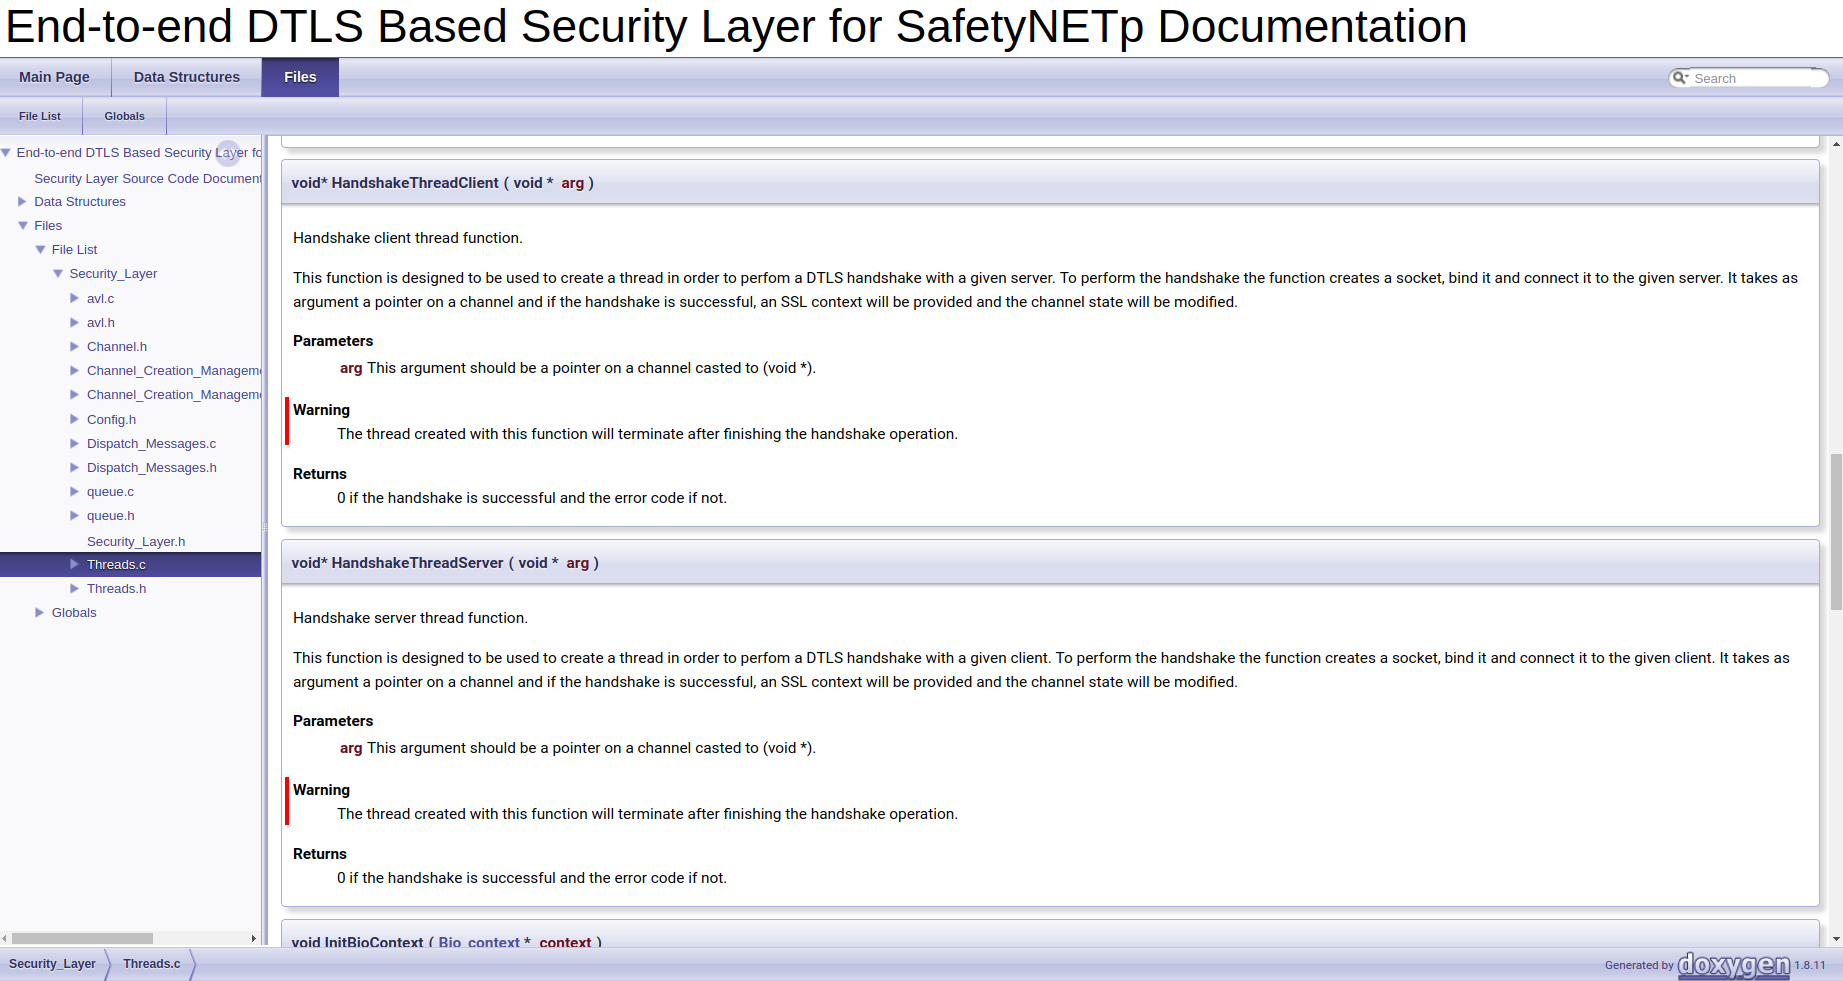
\includegraphics[width=19cm]{figures/realization/documentation_capture.png}
% \caption{Documentation capture}\label{documentation}
% \end{figure}


\subsection{Hardware Environment}

For the realization of this project, Pilz, the company which created SafetyNETp protocol, provided us with two Revolution Pis
containing their SafetyNETp implementation. The Revolution Pi (\autoref{revpi}) is a small computer designed by the Kunbus german company
based on the Rasberry Pi Compute Module. Unlike Rasberry Pi which is not designed for an industrial usage, the Revolution
Pi is designed to fit in industrial environments. As shown in \autoref{revpi_specs}, the Revolution Pi
has a protection against electrostatic discharge and electromagnetic interference according to the norms EN 61131-2 and IEC 61000-6-2.
In operating mode, the Revolution Pi could support a temperature between -40  $^\circ$C and +55 $^\circ$C which exceeds
the requirements of the norm EN 61131-2. The Revolution could be alimented by a power supply between 10.7 V and 28.8 V.
These characteristics make the Revolution Pi suitable for industrial usage \cite{revpi}.

\begin{table}[H]
    \begin{tabular}{|l|l|}
      \hline
      Processor & BCM2835, 700 MHz, single-core \\
      \hline
      RAM & 500 MByte \\
      \hline
      Electrostatic discharge protection & 4 kV / 8 kV (according to EN 61131-2 and IEC 61000-6-2) \\
      \hline
      Electromagnetic interference protection & Passed (according to EN 61131-2 and IEC 61000-6-2) \\
      \hline
      Surge/Burst tests & Passed (according to EN 61131-2 and IEC 61000-6-2) \\
      \hline
      Power supply &  min. 10.7 V - max. 28.8 V \\
      \hline
      Operating temperature & -40  $^\circ$C to +55 $^\circ$C(exceeds EN 61131-2 requirements) \\
      \hline
      Storage temperature & -40 $^\circ$C to +85 $^\circ$C (exceeds EN 61131-2 requirements) \\
      \hline
  \end{tabular}
  \caption[Revolution Pi characteristics]{Revolution Pi characteristics \cite{revpi}}
  \label{revpi_specs}
\end{table}

\begin{figure}[H]
\centering
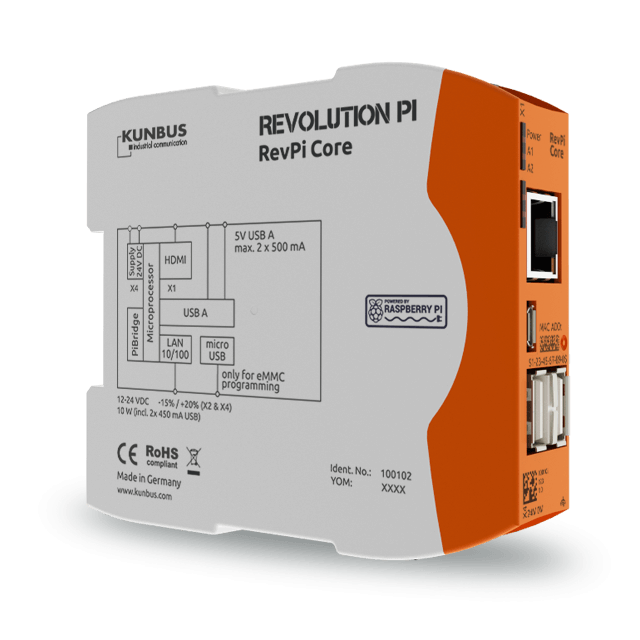
\includegraphics[width=9cm]{figures/realization/revpi.png}
\caption{Revolution Pi}\label{revpi}
\end{figure}

For the development, we used a laptop with the characteristics shown in \autoref{computer_characteristics}.

\begin{table}[H]
\centering
    \begin{tabular}{|l|l|}
      \hline
      Processor & Intel core i5 \\
      \hline
      RAM & 8 Gbyte \\
      \hline
      Graphics & Intel HD Graphics 620 \\
      \hline
  \end{tabular}
  \caption{Used computer characteristics}
  \label{computer_characteristics}
\end{table}

For interconnecting the Revolution Pis and our laptop we used a hub and Ethernet cables.

\section{Implementation}

In this section, we see the several steps we went through in order to implement our design.

\subsection{DTLS Implementation Choice}

Various DTLS implementations exists which support DTLS up to its final version, among these, we can cite:

\renewcommand{\labelitemi}{$\bullet$}
\begin{itemize}
\item \textbf{OpenSSL} \cite{OpenSSL}: This is an open source project that provides a robust, commercial-grade and
full-featured toolkit for SSL/TLS protocols. It is also a general-purpose cryptography library.
The OpenSSL toolkit is licensed under an Apache-style license, which basically means that
you are free to get and use it for commercial and non-commercial purposes subject to some
simple license conditions.

\item \textbf{WolfSSL} \cite{WolfSSL}: WolfSSL is a lightweight portable embedded SSL/TLS library written in ANSI C.
With its small size, speed, and feature set, WolfSSL targets embedded systems and resource-constrained environments.
It implements TLS and DTLS up to their latest versions which are currently TLS 1.2 and DTLS 1.2 and provides
progressive ciphers such as ChaCha20, Curve25519, NTRU, and Blake2b. This
software falls into the General Public License (GPL) and in case of commercial software
products, a commercial license must be bought.

\item \textbf{MatrixSSL} \cite{MatrixSSL}: MatrixSSL is an embedded SSL and TLS implementation designed for
small footprint IoT devices requiring low overhead per connection. The library is less than 50Kb on disk
with cipher suites. It includes client and server support through TLS 1.2, mutual authentication,
 and implementations of RSA, AES, SHA, SHA-256 and more.

\item \textbf{MbedTLS} \cite{MbedTLS}: formerly known as PolarSSL, it is an open source embedded SSL/TLS library provided by arm and written in C.
Its small memory footprint makes it suitable for embedded environments. MbedTLS provides an up to date implementations of both TLS and DTLS.
MbedTLS is primarily licensed under the Apache 2.0 license and a packaged version is available under the GPL as well.
Therefore MbedTLS could be used for free for both commercial and non-commercial use.
\end{itemize}

In fact, we decide to use MbedTLS for the following reasons \cite{MbedTLS}:

\renewcommand{\labelitemi}{$\bullet$}
\begin{itemize}
\item \textbf{Tiny and portable library}: As MbedTLS is written in C, it is portable and suitable for embedded environments.
\item \textbf{Easy to understand and use with a clean API}: MbedTLS offers a readable code and a logical,
clean, and well-documentated API. MbedTLS provides a reference and a high-level design for its API (using UML diagrams) making
understanding and using the library a lot easier.
\item \textbf{Easy to reduce and expand the code}: MbedTLS has no global code and has minimal coupling between its modules.
So it's easy to just grab a part and drop it into an existing project or add new functionality.
\item \textbf{Apache and GPL licenses}: MbedTLS could be used for free in open source and non-open source project
as well as in commercial and non-commercial projects.
\end{itemize}

\subsection{SafetyNETp Plugin Implementation for Wireshark}

To be able to understand the behavior of SafetyNETp devices, the first step was to analyze
the traffic exchanged between the two devices provided by Pilz. For this purpose, we used
the well-known traffic analyzer Wireshark. As SafetyNETp is proprietary protocol, it is difficult
to find information about its functioning or its packet format in public sources. In fact, Wireshark
does not recognize SafetyNETp packets, hence, the messages are shown as raw data. Analyzing raw data messages
makes our task extremely difficult. \autoref{safetynetp_raw_messages} shows a Wireshark capture of a data exchange between two
SafetyNETp devices. As the figure shows, no message type is mentioned, Wireshark just presents SafetyNETp's data
as UDP payload.


\begin{figure}[H]
\centering
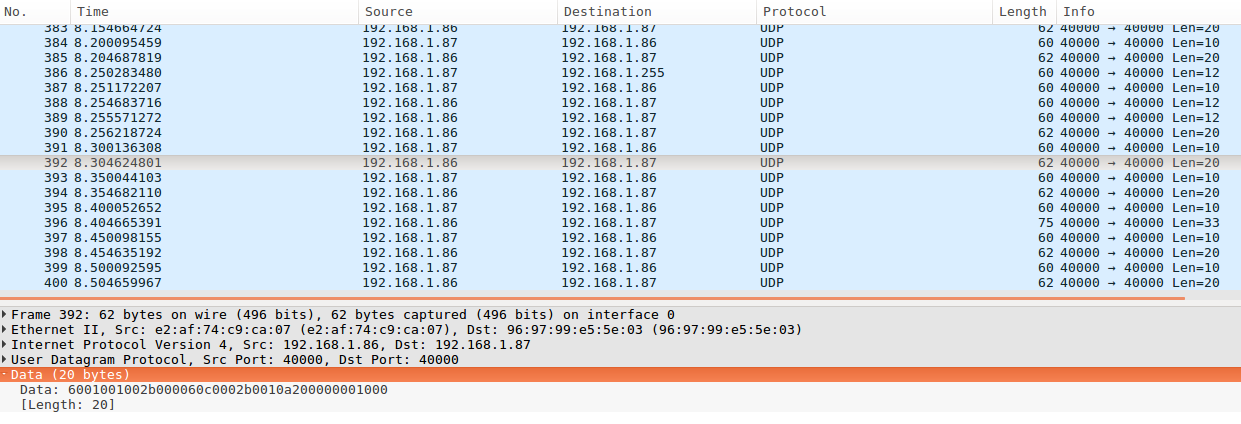
\includegraphics[width=17cm]{figures/realization/safetynetp_raw_messages.png}
\caption{Wireshark capture without our plugin}\label{safetynetp_raw_messages}
\end{figure}

To facilitate analyzing and debugging the exchanged messages, we implemented a Wireshark plugin using lua
programming language which enables the support of SafetyNETp in Wireshark. The \autoref{safety_plugin} shows a
capture after we have integrated our plugin into Wireshark. The exchanged messages are no longer shown as raw
UDP payload, instead, our plugin takes the responsibility for interpreting SafetyNETp packets and shows
their types. Furthermore, we are able to use filters, allowing for example to see only specific messages types.

\begin{figure}[H]
\centering
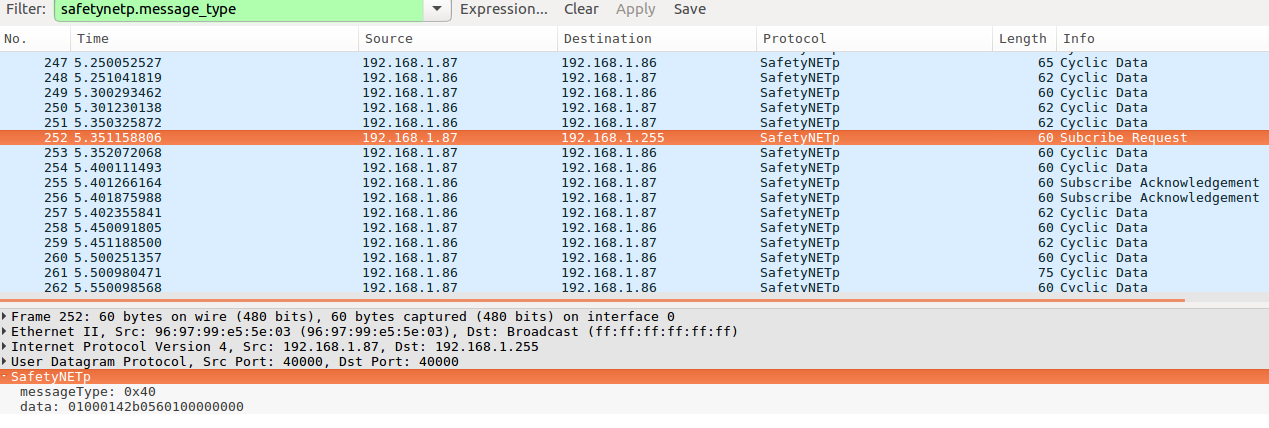
\includegraphics[width=17cm]{figures/realization/safety_plugin.png}
\caption{Wireshark capture after integrating our plugin}\label{safety_plugin}
\end{figure}

\subsection{Threads and Socket Managment}

As the Revolution Pis run Linux Debian, for exchanging data over the network,
SafetyNETp uses the Linux socket API. In fact, a socket is an abstraction through which an application
may send and receive data, in much the same way as an open file allows an application to read and write data.
A socket allows applications to communicate over the network, an information written to a socket
by an application on one machine can be read by an application on a different machine and
vice versa. Numerous types of sockets exist, for our case, we will be using UDP sockets.

Every SafetyNETp device using our security layer implementation runs several threads.
As shown in \autoref{sockets}, four kinds of threads are present:

\renewcommand{\labelitemi}{$\bullet$}
\begin{itemize}
\item \textbf{The first handshake thread}: This could be a client or a server thread, its role is to establish
the first handshake. This thread terminates when the handshake finishes.

\item \textbf{The receiving data thread}: This thread is responsible for receiving, decrypting, and verifying
data. The thread terminates when its session is closed.

\item \textbf{Session renewal thread}: This could be a client or a server thread, its role is to
establish a new handshake in order to renew the keying material. This thread terminates when the handshake
finishes or its session is closed.

\item \textbf{Sending data thread}: This thread is responsible for sending both protected and unprotected
data. This thread runs while the device is on.
\end{itemize}

In each device, one single thread exists for sending data, and $n$ threads exist for receiving data, with $n$
the number of channels. In fact for each connection, a \textit{first handshake thread} is created for establishing
the first handshake, then a \textit{receiving data thread} is created for receiving, decrypting, and verifying
data, furthermore, periodically, a \textit{session renewal thread} is created to renew the keying material.

For sending and receiving data, we have two possibilities, whether we create one single socket for all devices, or
create and dedicate a specific socket for each device. A socket has separate buffers for writing and reading
which means that it is possible to have two threads, one writing and one reading at the same time. However, having two
threads writing to a socket at the same time is not possible. We could have the case where a device is for example
establishing multiple handshakes with $n$ devices at the same. In this case, $n$ handshake threads will be running at the same
time. If we use one single socket, we need to manage the threads access for writing into the socket as it is not
possible to perform more than one write operation at the same time. Furthermore, when receiving a packet,
our application has to filter the incoming packets to know their sources as all the devices send their data
on the same socket. That's why, as shown in \autoref{sockets}, a separate socket is created for each device. Hence, having multiple
handshake threads does not cause access problem anymore as each thread will be writing on a separate socket. In
addition, no filtering is needed, the linux kernel will filter the packets according to the sockets.

\begin{figure}[H]
\centering
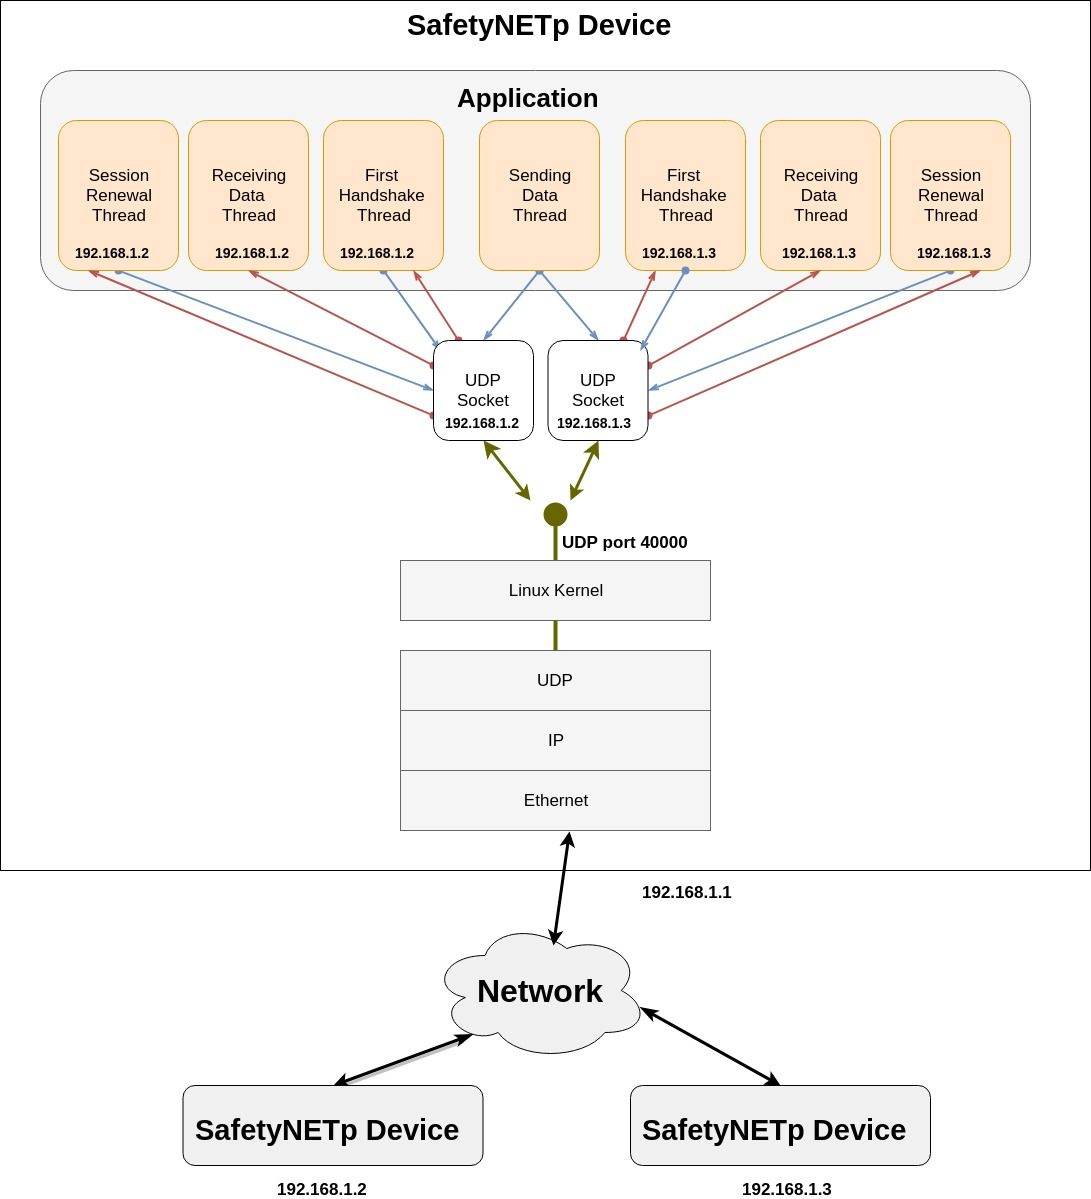
\includegraphics[width=13cm]{figures/realization/sockets.jpg}
\caption{Threads and sockets}\label{sockets}
\end{figure}

As mentioned in the previous chapter, we need to renew periodically the keying material to minimize cryptanalysis
attacks. This corresponds in our implementation to create a \textit{session renewal thread}. It is obvious that the \textit{session renewal thread} needs to write and read data from the dedicated socket. Meanwhile, the \textit{sending data thread} is
sending cyclically \textit{cyclic data} which means that it is writing to the socket. Therefore, we could end up
having simultaneous access to the socket. We can manage the simultaneous access by using a mutex variable to
protect writing on the socket, in fact, this solves the problem by letting only one thread writing at a time.
\autoref{mutex_write_socket} shows how the socket concurrent access is managed. If we assume that the green state is the
current, in this case, the \textit{sending data thread} will wait until the \textit{session renewal thread} writes and unlocks
the socket. Such management could delay sending \textit{cyclic data} that's why we need to avoid this method.

\begin{figure}[H]
\centering
\includegraphics[width=10cm]{figures/realization/write_to_queue.jpg}
\caption{Socket concurrent access}\label{mutex_write_socket}
\end{figure}

To avoid delaying \textit{cyclic data}, we will not allow the \textit{session renewal thread} to access the socket directly.
Instead, it writes the message on a queue and only the \textit{sending data thread} will have access to the sockets.
When the \textit{sending data thread} sends a message, it verifies the queue which contains the messages written by the
\textit{session renewal thread}. If the queue is not empty, the \textit{sending data thread} dequeues the first message and sends it.
Using this method, we ensure that the \textit{cyclic data} is sent immediately without any additional delay (\autoref{write_to_queue}).

\begin{figure}[H]
\centering
\includegraphics[width=8cm]{figures/realization/mutex_write_socket.jpg}
\caption{Prioritization of \textit{cyclic data} messages over handshake messages}\label{write_to_queue}
\end{figure}

\subsection{Channel Lookup}

Each SafetyNETp device can obviously communicate with multiple other devices. For instance, a publisher could
be publishing data for an arbitrary number of $n$ subscribers. The publisher will have a list of secure channels, each one is used
to communicate securely with one subscriber. Each channel has as an identifier the IP address of the subscriber.
For each \textit{cyclic data} message to be sent, the publisher has to fetch the list of channels and to find
the corresponding channel to use for the destination devices. Having a big number of channels
could affect the cycle time that’s why we will be interested in this section in selecting a search
algorithm that allows keeping the cycle time as it is as much as possible.

In order to find the channel to use, we need to find the one which has the corresponding IP address which is no
more than a 4 bytes integer. As a result, the problem is about finding an integer in a given list.
The classic method for searching is linear search, given a list of $n$ elements, it sequentially checks
each element of the list for the target value until a match is found or until all the elements have been
searched. the complexity of the linear search method is equal to $O(n)$.

% \begin{figure}[!htbp]
% \centering
% \includegraphics[height=2cm]{figures/design/linear_search.jpg}
% \caption{Linear search}\label{linear_search}
% \end{figure}

Another method is commonly used which is the binary search tree, it searches in a sorted list by
repeatedly dividing the search interval in half. Begin with an interval covering the whole list. If the
value of the search key is less than the item in the middle of the interval, narrow the interval to the
lower half. Otherwise, narrow it to the upper half. Repeatedly check until the value is found or the
interval is empty. The complexity of the binary search method is $O(log(n))$ if the tree is balanced, however,
if it is unbalanced it could reach a complexity of $O(n)$.

% \begin{figure}[H]
% \centering
% \includegraphics[height=7cm]{figures/design/binary_search_tree.jpg}
% \caption{Binary search tree}\label{binary_search_tree}
% \end{figure}

To get rid of the balancing problem, AVL is the solution. AVL tree is a self-balancing binary
search tree where the difference between heights of left and right subtrees cannot be more than one
for all nodes. Most of the binary search tree operations (search, max, min, insert, delete, etc) take
$O(h)$ time where $h$ is the height of the binary search tree. The cost of these operations may become
$O(n)$ for a skewed Binary tree where $n$ is the number of nodes. If we make sure that height of the tree remains $O(log(n))$ after every
insertion and deletion, then we can guarantee an upper bound of $O(log(n))$ for all these operations.
The height of an AVL tree is always $O(log(n))$ where $n$ is the number of nodes in the tree.

\begin{figure}[H]
\centering
\includegraphics[height=7cm]{figures/design/comparison_between_search_methods.png}
\caption{Comparison between $O(n)$ and $O(log(n))$}\label{comparison_between_search_methods}
\end{figure}

\autoref{comparison_between_search_methods} shows the two functions $n$ in red and $log(n)$ in blue it shows in
other words how increasing the number of elements will affect the number of comparisons to be performed in order
to find the target. It is clear that $log(n)$ is always below $n$ which means that the number
of comparisons is always smaller. As a result, we used the binary search tree method.

\section{Implementation Demo and Performance Test}

As shown in \autoref{test_environment}, our test environment consists of two Revolution Pis, a power supply and
a hub for interconnecting the Revolution Pis with our laptop.
The Revolution Pis are configured to subscribe mutually to each other, they have 192.168.1.86
and 192.168.1.87 as IP addresses.
In this section we go into an overview to see the implementation demo, then we move to the test.

\begin{figure}[H]
\centering
\includegraphics[width=10cm,height=6cm,frame]{figures/realization/test_environment.JPG}
\caption{Test environment}\label{test_environment}
\end{figure}

\subsection{Demo}

The \autoref{first_handshake} shows the case where the communication is initiated and the first handshake is established.
In fact, as we mentioned in the design chapter, the DTLS roles are chosen based on the IP addresses.
The right capture is the screen of the device which has the IP address 192.168.1.87 and left one
corresponds to the device which has the IP 192.168.1.86. As we can see the device with the higher IP launched
a server thread whereas the device with the smaller IP launched a client thread. After launching the threads,
they begin establishing the handshake and they exchange their certificates. Thereafter, each end-point
verifies the other end-point's certificate. As we see in this capture, the certificates are verified correctly and
therefore they start exchanging secured \textit{cyclic data}.

\begin{figure}[H]
\centering
\includegraphics[width=19cm,frame]{figures/realization/first_handshake(1).jpg}
\caption{The first handshake establishment}\label{first_handshake}
\end{figure}

In order to minimize the risk of cryptanalysis attacks, as mentioned in the previous chapter,
a new handshake is run each a well defined period of time. For test purposes, we set the period of session renewal
to 20 seconds. As shown in \autoref{session_renewal_threads}, each 20 seconds the devices launch a \textit{renewal session thread}
in order to establish a new handshake. Following each established handshake, the \textit{channel id} header
field is incremented to allow the receiving devices to verify and decrypt the messages with right keying
material.

\begin{figure}[H]
\centering
\includegraphics[width=19cm,frame]{figures/realization/session_renewal(2).png}
\caption{Session renewal threads}\label{session_renewal_threads}
\end{figure}

The main difference between the \textit{first handshake thread} and the \textit{renewal session thread} is
that while establishing the first handshake the cyclic data is blocked as the identity of
the second end-point could not be verified before
finishing the handshake. However, when renewing the keying material, the cyclic data is sent,
and the new handshake's messages should be sent without interrupting sending cyclic data.
The \autoref{cyclic_data_time_out} shows the message which SafetyNETp application layer logs when
the timeout of the cyclic data expires. As shown in \autoref{session_renewal_threads} no such message
is logged which confirms that the handshakes are being established without interrupting sending the cyclic data.

\begin{figure}[H]
\centering
\includegraphics[width=10cm]{figures/realization/cyclic_data_time_out.png}
\caption{SafetyNETp timeout log}\label{cyclic_data_time_out}
\end{figure}

The \autoref{safetynetp_original_message} shows a Wireshark capture of a cyclic data message sent unprotected as plaintext
before integrating our security
layer. The \autoref{secured_cyclic_data_message} shows a Wireshark capture of a cyclic data message sent through our security layer.
The first byte of the secured message is the security layer frame byte which is, in this case, \textit{0x88},
we chose arbitrarily this value and it could be changed via a configuration file. The second byte is the channel id
and the rest of the message is the SafetyNETp cyclic data message encapsulated into a DTLS frame.
We remark that the secured message is longer than the original message which is obvious as
additional data are included for encryption and for integrity checks.

\begin{figure}[H]
\centering
\includegraphics[width=12cm,frame]{figures/realization/unprotected_cyclic_data.png}
\caption{SafetyNETp original cyclic data message}\label{safetynetp_original_message}
\end{figure}

\begin{figure}[H]
\centering
\includegraphics[width=12cm,frame]{figures/realization/secured_cyclic_data.png}
\caption{Secured cyclic data message}\label{secured_cyclic_data_message}
\end{figure}

In our security layer, when performing the DTLS handshake the devices' identities are verified using the certificate mechanism.
Therefore we have created our own \ac{PKI} in order to issue the devices' certificates. Our public key infrastructure
is composed from two \ac{CA}s, a root \ac{CA} and an intermediate \ac{CA}. The first step was to create the root CA by
generating its public and private keys and generating its certificate. In fact, the root CA's certificate is self-signed as it is
the first created CA. The second step was to create the intermediate CA, like creating the root CA, we generated the
public and the private keys as well as the certificate. However, the intermediate CA's certificate is not self-signed, it is actually
signed by the root CA. One could ask why do we need an intermediate CA when only the root CA is sufficient? In fact, it is a best practice to create an intermediate CA. The intermediate CA is used to issue and sign certificates on behalf of
the root CA. This minimizes the risks of compromising the root CA's private key.
After the creating the CAs, we issued a certificate for each device, thereafter, we configured the devices and added the root CA among the list of trusted CAs.
Creating the CAs as well as issuing the certificates is performed using three bash scripts that we have developed.
\autoref{cert_example} shows a certificate example which is, in this case, the intermediate CA's certificate.

\begin{figure}[H]
\centering
\includegraphics[width=12cm,frame]{figures/realization/certificate_example.png}
\caption{Certificate example}\label{cert_example}
\end{figure}

In order to facilitate modifying the parameters of the security layer, we created the configuration file
shown in \autoref{config_file}. Through this configuration file, SafetyNETp developers could easily change the security layer frame
byte, set the interval for renewing the keying material, set the max channel id value, print the sent and the received messages and print threads log to facilitate
debugging.

\newpage

%-------------------------------------------------------------------------------
%
%       Filename:  listing_two.tex
%
%    Description:  The file shows a hack for the use of lstlisting package with
%                  IfLanguagepackage
%
%        Version:  0.1
%        Created:  02.05.2016
%       Revision:  none
%
%         Author:  M.Sc. Oliver Kehret, oliver.kehret@hs-offenburg.de
%   Organization:  ivESK, Offenburg University, Germany
%      Copyright:  Copyright (c) 2016, M.Sc. Oliver Kehret
%
%-------------------------------------------------------------------------------
\begin{lstlisting}[caption={Security layer configuration file},label={config_file}]
/**
 * @brief Set Security Layer Frame byte value
 */
#define SECURITY_LAYER_FRAME_BYTE             0x88
/**
 * @brief Configure the renewing session interval in seconds
 */
#define RENEWING_SESSION_INTERVAL              20
/**
 * @brief Configure the period of time to wait after renewing the session to
 * switch using the new DTLS context
 */
#define DTLS_CONTEXT_SWITCH_TIME               4
/**
 * @brief Set the max value for the channel ID, when this value is reached
 * the next value will be 0x00
 */
#define MAX_CHANNEL_ID_VALUE                   0xff
/**
 * @brief Define this macro to print the Handshakes log
 */
#define PRINT_HANDSHAKE_LOG
/**
 * @brief Define this macro to print the Threads log
 * (Server and Client IP, channel ID, renewing session timer)
 */
#define PRINT_THREADS_LOG
/**
 * @brief Define this macro to print the outgoing messages (plaintext)
 */
#define PRINT_O_MSG
/**
 * @brief Define this macro to print the incoming messages (plaintext)
 */
#define PRINT_I_MSG
\end{lstlisting}




\subsection{Performance Test}

In this section, we present the results of the performed tests which consist of evaluating SafetyNETp with and
without the security layer. For this purpose, we have generated random messages with different lengths and we have calculated the time needed for sending and receiving them. In order to have more accuracy,
we have calculated the send and the receive time  1000 times for each length. The results presented in
the following graphs show the average value for each message length.

As a first step, we started by evaluating SafetyNETp before integrating the security layer.
\autoref{original_safetynetp} shows the time needed for sending and receiving the messages.

\begin{figure}[H]
\centering
\includegraphics[width=19cm,frame]{figures/realization/original_safetynetp.jpg}
\caption{SafetyNETp before integrating the security layer}\label{original_safetynetp}
\end{figure}


As a second step, we evaluated our security layer.
\autoref{safetynetp_with_scurity_layer} shows the time needed for sending and receiving messages through the
security layer using TLS\_RSA\_WITH\_AES\_128\_CBC\_SHA256 cipher suite. The time includes the encryption, the MAC
calculation and the decryption.

\begin{figure}[H]
\centering
\includegraphics[width=19cm,frame]{figures/realization/safetynetp_with_scurity_layer.jpg}
\caption{SafetyNETp after integrating the security layer}\label{safetynetp_with_scurity_layer}
\end{figure}

The protected messages are encapsulated into DTLS frames then into the security layer frame. This introduces
a data overhead as the secured messages contain the security layer and DTLS headers as well as the MAC.
Furthermore, some encryption algorithms need to add padding to the messages. \autoref{data_overhead} shows the
data overhead.

\begin{figure}[H]
\centering
\includegraphics[width=19cm,frame]{figures/realization/data_overhead.jpg}
\caption{Data overhead}\label{data_overhead}
\end{figure}

The startup time of the system without our security layer is equal to the startup time of the SafetyNETp devices
as the devices start exchanging \textit{cyclic data} directly after the startup. However, with our security layer, after the startup,
the devices establish the DTLS handshake before exchanging \textit{cyclic data}. In fact, as shown in \autoref{startup_time_overhead}
the time needed for the devices' startup is equal to \textit{94 seconds}, the time needed to establish the DTLS handshake is equal to
\textit{7 seconds}. Therefore the new startup time is equal to \textit{101 seconds}.


\begin{figure}[H]
\centering
\includegraphics[width=10cm,frame]{figures/realization/startup_time_overhead.jpg}
\caption{Startup time overhead}\label{startup_time_overhead}
\end{figure}


%
% In order to evalute our solution, we performed some perfomance measures by sending 300 messages before
% and after integrating our security layer. In fact, as shown in \autoref{enc_dec_overhead}
% in order to encapsulate the original SafetyNETp message into the security layer frame wich includes
%  encrypting the message, performing
% the MAC calculation, encapsulating the message into DTLS frame and then into the security layer frame,
% the average needed time is \textit{340 microseconds}, the maximum time we have encoutered is \textit{448 microseconds} and the minimun time is \textit{236 microseconds}.
% In order to decapsulate a secured frame wich includes the decryption,the identity and the integrity checks, the average needed
% time is \textit{120 microseconds}, the maximum time is \textit{170 microseconds} and the minimum time is \textit{100 microseconds}.
% As we are using 100 Mbit/second Ethernet, the transmission overhead is insignificant, in fact, it is equal to \textit{2 microseconds}.
% To conclude the maximum total overhead introduced by our security layer is no more than \textit{620 microseconds}.
%
% \begin{figure}[H]
% \centering
% \includegraphics[width=15cm]{figures/realization/enc_dec_overhead.png}
% \caption{Overhead introduced in encapsulating and decapsulating messages}\label{enc_dec_overhead}
% \end{figure}
%
% The startup time of the system without our security layer is equal to the startup time of the SafetyNETp devices
% as the devices start exchanging \textit{cyclic data} directly after the startup. However, with our security layer, after the startup,
% the devices establish the DTLS handshake before exchanging \textit{cyclic data}. In fact, as shown in \autoref{statup_time_overhead}
% the time needed for devices' startup is equal to \textit{94 seconds}, the time needed to estbalish the DTLS handshake is equal to
% \textit{7 seconds}. Therefore the new startup time is equal to \textit{101 seconds}.
%
% \begin{figure}[H]
% \centering
% \includegraphics[width=15cm]{figures/realization/statup_time_overhead.png}
% \caption{Startup time overhead}\label{statup_time_overhead}
% \end{figure}
%
% \begin{figure}[H]
% \centering
% \includegraphics[width=19cm]{figures/realization/test.jpeg}
% \caption{Startup time overhead}\label{test}
% \end{figure}

\section*{Conclusion}

 Throughout this chapter, we presented the software and the hardware environments, we outlined the
 important implementation steps and we evaluated finally the performance of our solution.

%_____________________________________________________________________________________
%
%       Filename:  Conclusion.tex
%
%    Description:  Thesis Template HS Offenburg
%
%
%         Author:  Okba ZOUEGHI, okba.zoueghi@gmail.com
%     Supervisor:  Andreas Walz, Chadlia Jerad
%   Organization:  HS Offenburg, Offenburg, Germany
%
%_____________________________________________________________________________________

\chapter*{General Conclusion and Perspectives}
\addcontentsline{toc}{chapter}{General Conclusion}
\markboth{General Conclusion and Perspectives}{}

Today, most of the currently available industrial networks focus mainly on meeting real-time requirements and are designed and developed
without any built-in security. SafetyNETp is one of the well known and most used Industrial Ethernet protocols, although it does not
provide any special security measures. SafetyNETp based networks are vulnerable to attacks as it enables unauthorized access in a
relatively straightforward manner given that all the communications are performed with no authentication, no integrity checks, and no encryption.

Designing and implementing a security layer for SafetyNETp from scratch is a difficult and very error-prone task.
That's why we were interested in our project by the available protocols which are already tested and assessed by the internet community.
DTLS and IPsec were the candidate protocols to be used. In fact, our protocol of choice was DTLS, this is mainly because DTLS is situated at the session layer
whereas IPsec is situated at the network layer. Actually, this makes DTLS a lot easier to integrate.

The implemented DTLS based security layer provides confidentiality, integrity, and authenticity respectively by
using encryption, MAC algorithms, and certificates. It is obvious that a time and a data overhead will be introduced by
running those security mechanisms. In fact, the performance tests have shown that the time needed for sending
and receiving a message over the security layer is around 7 milliseconds using
TLS\_RSA\_WITH\_AES\_128\_CBC\_SHA256 cipher suite.

SafetyNETp provides two communication models compatible with each other which are RTFN and RTFL. RTFN is
used when a cycle time over 1 millisecond is sufficient whereas RTFL provides a cycle time at microsecond
level. The current design and implementation of the security layer concerns only RTFN and does not provide
any security to RTFL. Therefore, the communication between the secured RTFN and RTFL is not
possible. In fact, Securing RTFL needs entirely a new design, moreover, as RTFL time constraints are more
tight, integrating a security layer may affect significantly its cycle time.

%}%
%
%
%
%
%
%-------------------------------------------------------------------------------
%	Appendix
%-------------------------------------------------------------------------------
% add possible appendix
% \appendix
% \addpart{Appendix}
\setcounter{figure}{0}
\renewcommand\thefigure{A.\arabic{figure}}
% \include{chapter/appendixa}
\renewcommand\thefigure{B.\arabic{figure}}
% \include{chapter/appendixb}
% \renewcommand\thefigure{C.\arabic{figure}}
% \include{chapter/appendixc}
%-------------------------------------------------------------------------------
%	Bibliography
%-------------------------------------------------------------------------------
%
%\nocite{*}
\printbibliography
%
%
%-------------------------------------------------------------------------------
%	\end{document}
%-------------------------------------------------------------------------------
\end{document}
